\documentclass[oneside]{book}
% Título y autor(es):
\title{Resumen de Física III A (62.05)}
\author{Menéndez Martín}

\usepackage[spanish]{babel}
\usepackage{amsmath}
\usepackage[a4paper,headheight=16pt,scale={0.7,0.8},hoffset=0.5cm]{geometry}
\usepackage{pdfpages}
\usepackage[utf8]{inputenc}
\usepackage{lastpage}
\usepackage{float}
\usepackage{listings}
\usepackage{anysize}
\usepackage{listings}
\numberwithin{equation}{section}
\numberwithin{figure}{section}
\numberwithin{table}{section}
\usepackage{fancyhdr}
\usepackage[hang,bf]{caption}
\usepackage{graphicx}
\usepackage{circuitikz}
\usepackage{tikz}
\usepackage[spanish]{varioref}
\usepackage{hyperref}
\usepackage{xcolor}\hypersetup{linkbordercolor=white}
\usepackage{cancel}

\pdfcompresslevel=9
\newcommand{\imgdir}{includes}
\graphicspath{{\imgdir/}}

\everymath{\displaystyle}
\newcommand{\vect}[1]{\underline{\textbf{#1}}}
\newcommand{\bayes}{\mathop{\lessgtr}}


%------------------------- Inicio del documento ---------------------------

\begin{document}
% Hago que en la cabecera de página se muestre a la derecha la sección, y en el pie, en número de página a la derecha:
\pagestyle{fancy}
\renewcommand{\sectionmark}[1]{\markboth{}{\thesection\ \ #1}}
\lhead{}
\chead{}
\rhead{\rightmark}
\lfoot{Física III A (62.05)}
\cfoot{}
\rfoot{P\'agina \thepage\ de \pageref{LastPage}}
% Carátula:
\begin{titlepage}

\thispagestyle{empty}

\begin{center}

\includegraphics[scale=0.3]{fiuba}\\
\large{\textsc{Universidad de Buenos Aires}}\\
\large{\textsc{Facultad De Ingeniería}}\\
\small{A\~no 2013 - 2\textsuperscript{do} Cuatrimestre}
\end{center}

\begin{center}
\Large{\underline{\textsc{Física III A (62.05)}}}

\vspace*{2cm}

\textbf{\begin{LARGE}
Resumen de Física III A\\
\end{LARGE}}
\end{center}

\vspace*{3cm}

\begin{tabbing}
\hspace{2cm}\=\+
\\
	INTEGRANTE:\hspace{-1cm}\=\+\hspace{1cm}\=\hspace{6cm}\=\\
		Menéndez, Martín Nicolás	\>\>- \ 92830\\
		$\langle$menendez91@live.com.ar$\rangle$\\
		\\
		Ing Gama,Fernando
\end{tabbing}
\end{titlepage}
% Hago que las páginas se comiencen a contar a partir de aquí:
\setcounter{page}{1}
% Pongo el índice en una página aparte:
\tableofcontents
%\listoffigures
%\listoftables
\newpage
% Inicio del TP:
\marginsize{1cm}{1cm}{1cm}{1cm}
\setcounter{chapter}{0}

\part{Física Cuántica}

	\chapter{Ondas}
		\section{Ecuación de onda}
			Ecuación diferencial en derivadas parciales lineal de segundo orden que describe la propagación de ondas.
			
			\begin{center}
			\boxed{\displaystyle \frac{\partial^2 U(\vec{r},t)}{\partial t^2}=c^2\overrightarrow{\nabla}^2U(\vec{r},t)}
			\end{center}
	
			Donde $c$ es equivalente a la velocidad de propagación de la onda.
			
			\subsection{Soluciones generales}
			
				Son de la forma $\displaystyle U(\vec{r},t)=Ae^{i(k\vec{r}-wt)}$ para una onda que se propaga. Puede verificarse que:\\
				
				\begin{center}
				$\displaystyle \frac{\partial^2 U(\vec{r},t)}{\partial t^2}=Aw^2U(\vec{r},t)$ y $\displaystyle \overrightarrow{\nabla}^2U(\vec{r},t)=Ak^2U(\vec{r},t) \Rightarrow c=\frac{w}{k}$
				\end{center}
				
				Siendo $w$ la frecuencia angular y $k$ el número de onda asociada.
			
			\subsection{Ejemplo de la cuerda vibrante}

				Teniendo la solución de la ecuación de onda unidimensional incluyendo la propagación en ambas direcciones: $\displaystyle U(x,t)=Ae^{i(kx-wt)}+Be^{-i(kx+wt)}$.Siendo el sistema una cuerda de largo $L$ sujeta a las condiciones de contorno $U(0,t)=0$ y $U(L,t)=0$ y su condición inicial $U(x,0)=f(x)$. Se obtiene:\\
				
				$\displaystyle U(0,t)=Ae^{i(k*0-wt)}+Be^{-i(k*0+wt)}=0 \Rightarrow Ae^{-iwt}+Be^{-iwt}=0 \Rightarrow B=-A$\\
				
				$\displaystyle U(x,t)=Ae^{i(kx-wt)}-Ae^{-i(kx+wt)}=A(e^{ikx}-e^{-ikx})e^{-iwt}=2Ai\sin (kx)e^{-iwt}$\\
				
				$\displaystyle U(L,t)=2Ai\sin (kL)e^{-iwt}=0 \Rightarrow kL=n\pi \Rightarrow \frac{n\pi}{L} $\\
				
				$\displaystyle U(x,t)=2Ai\sin (\frac{n\pi}{L}x)e^{-iwt}$\\
				
				$\displaystyle U(x,0)=2Ai\sin (\frac{n\pi}{L}x)=f(x) \Rightarrow U(x,t)=f(x)e^{-iwt}$\\			
							
		\section{Superposición}
			\subsection{Interferencia}
			
			Fenómeno en el que dos o más ondas se superponen para formar una onda resultante, que puede presentar amplificación, disminución o neutralización del movimiento.\\
			
			Considerando dos ondas definidas por $\displaystyle Y_1(x,t)=Ae^{i(kx-wt)}$ y $\displaystyle Y_2(x,t)=Ae^{i(kx+wt)}$, se puede calcular su superposición como:\\
			
			$\displaystyle Y_1(x,t)+Y_2(x,t)=Ae^{i(kx-wt)}+Ae^{i(kx+wt)}=A(e^{iwt}+e^{-iwt})e^{ikx}=2A\cos (wt)e^{ikx}$\\
						
			\subsection{Batidos}
			
			Fenómeno en el que dos ondas de frecuencias similares se superponen, generando una onda resultante de amplitud modulada.\\
			
			Considerando dos ondas definidas por $\displaystyle Y_1(x,t)=Ae^{i(kx-w_1t)}$ y $\displaystyle Y_2(x,t)=Ae^{i(kx-w_2t)}$, se puede calcular su superposición como:\\
			
			$\displaystyle Y_1(x,t)+Y_2(x,t)=Ae^{i(kx-w_1t)}+Ae^{i(kx-w_2t)}=Ae^{ikx}(e^{-iw_1t}+e^{-iw_2t})$\\
			
			Podemos escribir $w_1=\frac{1}{2}(w_1+w_2)+\frac{1}{2}(w_1-w_2)$ y $w_2=\frac{1}{2}(w_1+w_2)-\frac{1}{2}(w_1-w_2)$\\
			
			$\displaystyle Y_1(x,t)+Y_2(x,t)=Ae^{ikx}e^{-i\frac{1}{2}(w_1+w_2)t}(e^{i\frac{1}{2}(w_1-w_2)t}+e^{-i\frac{1}{2}(w_1-w_2)t})=Ae^{ikx}e^{-i\frac{1}{2}(w_1+w_2)t}2\cos(\frac{w_1-w_2}{2}t)$\\
			
			$\displaystyle Y_1(x,t)+Y_2(x,t)=2Ae^{i(kx-\frac{w_1+w_2}{2}t)}\cos (\frac{w_1-w_2}{2}t)$\\
			
		\section{Paquetes de onda}
				\subsection{Velocidad de fase}
				\subsection{Velocidad de grupo}
		\nopagebreak
	\chapter{Fenómenos experimentales}	
		\section{Efecto fotoeléctrico}
			Heinrich Hertz descubrió entre 1886 y 1887 mediante un experimento que una descarga eléctrica entre dos electrodos ocurre más fácilmente cuando sobre uno de ellos incide luz ultravioleta, debido a que ocasiona la emisión de electrones desde la superficie del cátodo. A esta emisión se le denomina \textbf{efecto fotoeléctrico}.
			
			\begin{figure}[H]
				\begin{center}
				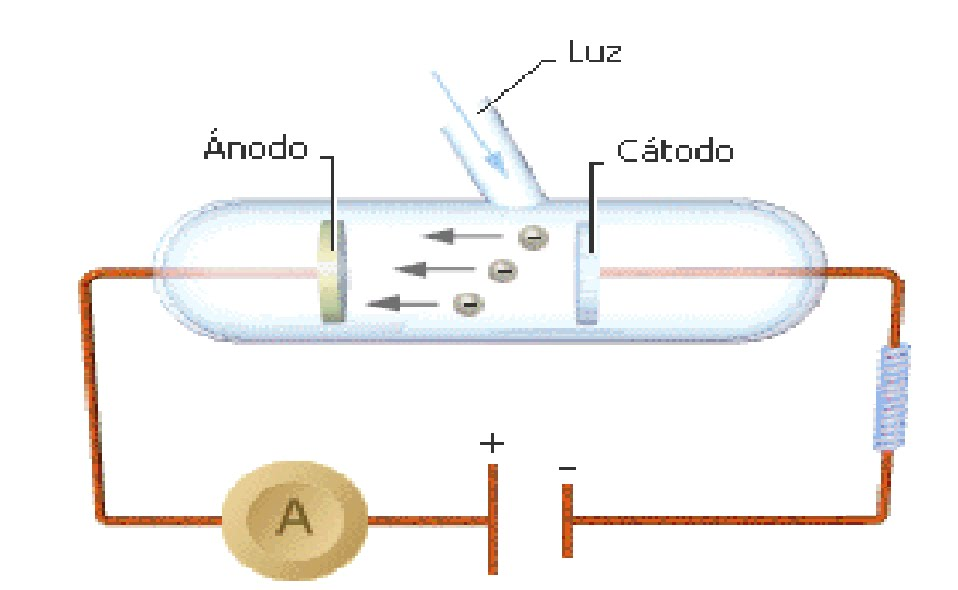
\includegraphics[scale=0.25]{Fotoelectrico.jpeg} 
				\caption{Circuito para estudiar el efecto fotoeléctrico}
				\end{center}
			\end{figure}
		
			Una envoltura de vidrio encierra el aparato en un espacio vacío, la luz monocromática incidente a través de una ventana de cuarzo sobre la placa de metal (cátodo)	y esta libera electrones (fotoelectrones). Si estos son atraídos al ánodo de metal mediante una diferencia de potencial $V$ aplicada entre cátodo y ánodo, se podrían detectar como una corriente mediante el amperímetro.\\
			
			Invirtiendo el signo de $V$, la corriente no cae inmediatamente a cero, lo cuál sugiere que los electrones son emitidos desde el cátodo con energía cinética, por lo que algunos alcanzarán el ánodo sin importar que el campo eléctrico se oponga a su movimiento. Existe un valor $V_0$ llamado \textbf{Potencial de frenado} para el cual la corriente fotoeléctrica es nula. Es decir, la energía cinética de los fotoelectrones más rápidos es contrarestada por la energía producto del potencial. \boxed{K_{max}=eV_0}\\
			
			Características fundamentales:
			
			\begin{enumerate}					
			\item Experimentalmente $K_{max}$ es independiente de la intensidad de la luz, aunque la teoría clásica exige que la energía cinética del electrón debería aumentar de acuerdo con el aumento de la intensidad del haz luminoso.
			\item Según la teoría clásica, el efecto fotoeléctrico debería ocurrir para cualquiera frecuencia de la luz, pero experimentalmente para cada superficie existe una frecuencia de corte $\upsilon_0$ a partir de la cuál ocurre el fenómeno.
			\item En la teoría clásica la energía luminosa se encuentra uniformemente distribuida sobre el frente de onda. Entonces si esta es lo suficientemente débil existirá un tiempo de retraso mensurable entre el instante en que la luz empieza a incidir sobre la superficie y la expulsión del fotoelectrón. Experimentalmente nunca se ha medido un tiempo de retraso mensurable.
			\end{enumerate}			
					
			\subsection{Ecuación de Einstein}
			
				Einstein supuso que durante el proceso un fotón es completamente absorbido por un electrón del cátodo. La energía cinética del electrón emitido es $K=h\upsilon-w$, siendo $h\upsilon$ la energía del fotón incidente y $w$ es el trabajo necesario para sacar al electrón del metal.\\
				
			\subsection{Función trabajo, frecuencia y longitud de onda umbral}
			
				En el caso de que el enlace sea el más débil y no existan pérdidas internas, el fotoelectrón emergerá con la energía cinética máxima:
				
				\begin{center}
				\boxed{K_{max}=h\upsilon-w_0}
				\end{center}
			
				Donde $w_0$ es la energía característica del metal denominada \textbf{Función trabajo}\\
			
				Duplicando la intensidad, se duplican el número de fotones y por ende la corriente eléctrica, en concordancia con los resultados empíricos.\\				
				
				Partiendo de $K_{max}=eV_0=h\upsilon-w_0$, cuando la energía cinética es nula, $h\upsilon_0=w_0 \Rightarrow \upsilon_0=\frac{w_0}{h}$. Siendo $\upsilon_0$ la \textbf{Frecuencia umbral}, luego $\lambda_0=\frac{c}{\upsilon_0}$ será la \textbf{Longitud de onda umbral}.\\			
			
			\subsection{Concepto de Fotón}
			
			Propuso también que la energía radiante estaba cuantizada en paquetes concentrados, los cuales posteriormente se llamaron \textbf{fotones}, que viajan como ondas clásicas.
				Dicho paquete de energía se supuso localizado en un volumen de espacio pequeño y se mantiene localizado mientras se mueve alejándose de la fuente con velocidad $c$. La energía del paquete es proporcional a su frecuencia mediante:
				
				\begin{center}
				\boxed{E=h\upsilon}
				\end{center}
			
			\subsection{Aplicaciones técnicas}
						
				\begin{itemize}
					\item Producción de energía eléctrica por radiación solar
					\item Aprovechamiento energético de la energía solar. 
					\item Fabricación de células utilizadas en los detectores de llama de las calderas de las grandes centrales termoeléctricas.
					\item Sensores utilizados en las cámaras digitales. 
					\item Diodos fotosensibles tales como los que se utilizan en las células fotovoltaicas y en electroscopios o electrómetros.
					\item Diodos LED de iluminación
				\end{itemize}										
			
		\section{Rayos X}
			\subsection{Espectro continuo}
			\subsection{Longitud de onda de corte}
			\subsection{Difracción}	
			\subsection{Condición de Bragg}
		\section{Relatividad espacial}
		
		\textbf{Situación clásica:} Newton, Maxwell, Transformación de Galileo. Había un pequeño problema con la velocidad de la luz, que daba igual en cualquier sistema y no se condecía con la transformación de Galileo.

		\textbf{Einstein:} Generalizó la inercialidad de los sistemas de referencias y empezó a modificar la transformación de galileo. Descartando la idea de que el tiempo es el mismo en cualquier sistema de referencia. De esta forma definió la simultaneidad en base a la velocidad de la luz.

		\textbf{Soluciones de Einstein:}
		\begin{itemize}
			\item Las direcciones perpendiculares al movimiento de los sistemas de referencia, se conservan.
			\item Los tiempos de eventos que ocurren en el mismo lugar tienen una diferencia de $1/\sqrt{1-v^{2}/c^{2}}$ respecto de cada sistema de referencia. El \emph{proper time} es el medido por el sistema de referencia que observa al evento ocurrir en el mismo sitio.
			\item Las direcciones medidas paralelas al movimiento de los sistemas de referencia difieren en una cantidad $\sqrt{1-v^{2}/c^{2}}$. La longitud medida desde el sistema de referencia que está quieto es la \emph{proper length}.
\end{itemize}

\begin{center}
$x=vt+x^\prime \sqrt{1-v^{2}/c^{2}}$

$x^\prime=\frac{x-vt}{\sqrt{1-v^{2}/c^{2}}}$

$t=\frac{t^\prime+x^\prime v/c^{2}}{\sqrt{1-v^{2}/c^{2}}}$

$t^\prime=\frac{t-xv/c^{2}}{\sqrt{1-v^{2}/v^{2}}}$

$y^\prime=y$ 

$z^\prime=z$
\end{center}

Hay que suponer que la masa es una función de la velocidad sino las ecuaciones de Newton NO cierran, y las de Maxwell tienen que cerrar sí o sí ya que Einstein enunció que la velocidad de la luz no varía.\\

La masa es $m(v)=\frac{m_{0}}{\sqrt{1-v^{2}/c^{2}}}$ y la energía relativista de una partícula es $E(v)=E_{c}(v)+E(0)$. Siendo $E(0)$ la energía intrínseca de la partícula y $E_{c}(v)$ la energía cinética.\\

\begin{center}
	$E(v)=mc^2 \textrm{   y   } E(0)=m_0 c^2$
\end{center}

Esto lleva a que la masa relativista es una medida de la energía contenida en una partícula.

\begin{center}
	$E^2(p)=(c p)^2+m_0^2 c^4$
\end{center}

La energía intrínseca no altera la mecánica clásica porque se agregaría como suma en ambos lados de la ecuación.			
		
		\section{Efecto Compton}
					
			Analizando una sola colisión fotón electrón, para una radiación de frecuencia $\upsilon$, la energía de un fotón en el haz incidente es $E=h\upsilon$. Considerando al fotón como un paquete de energía localizado, como una partícula de energía total relativista $E$ puramente cinética, impulso $p=E/c=h\upsilon/c=h/\lambda$ y masa en reposo nula.\\
			
			Dicho fotón colisiona elásticamente contra un electrón libre e inicialmente estacionario, conservandose el momento lineal del sistema y la energía total, dispersádose el fotón con un ángulo $\theta$ con una longitud de onda $\lambda^\prime$ mientras que el electrón emerge a un ángulo $\varphi$.\\

\begin{minipage}[t]{0.5\textwidth}
	\begin{itemize}
		\item Estado inicial
			\begin{itemize}
				\item Electrón
					\begin{itemize}
						\item $E=m_0c^2$
						\item $p=0$
					\end{itemize}
				\item Fotón
					\begin{itemize}
						\item $E_0=h\upsilon$
						\item $p_0=h/\lambda$
					\end{itemize}
			\end{itemize}
	\end{itemize}						
\end{minipage}
\begin{minipage}[t]{0.5\textwidth}
	\begin{itemize}
		\item Estado final
			\begin{itemize}
				\item Electrón
					\begin{itemize}
						\item $E=\sqrt{m_0^2c^4+p^2c^2}$
						\item $p=p$
					\end{itemize}
				\item Fotón
					\begin{itemize}
						\item $E_1=h\upsilon^\prime$
						\item $p_1=h/\lambda^\prime$
					\end{itemize}
			\end{itemize}
	\end{itemize}						
\end{minipage}\\
\\
		Por la conservación del momento se tiene:\\
		
			\begin{center}
				\begin{minipage}[t]{0.25\textwidth}
					$p_0=p_1\cos \theta + p\cos \varphi$\\
					$(p_0-p_1\cos \theta)^2=p^2\cos^2 \varphi$\\
				\end{minipage}
				\begin{minipage}[t]{0.25\textwidth}
					$p_1\sin \theta = p\sin \varphi$\\
					$p_1^2\sin^2 \theta=p^2\sin^2 \varphi$\\
				\end{minipage}
			\end{center}
			\begin{center}
			Sumando ambos $p_0^2+p_1^2-2p_0p_1\cos \theta=p^2$\\
			\end{center}
			
		Por la conservación de la energía relativista total: $E_0+m_0c^2=E_1+K+m_0c^2 \Rightarrow E_0-E_1=K=c(p_0-p_1)$\\
		
		Siendo la energía relativista $E^2=c^2p^2+(m_0c^2)^2$ entonces $p^2=(K/c)^2+2Km_0$, se puede reemplazar $p^2$ y $K$ de las expresiones anteriores para obtener:\\
		
		$(p_0-p_1)^2+2m_0c(p_0-p_1)=p_0^2+p_1^2-2p_0p_1\cos \theta \Rightarrow m_0c(p_0-p_1)=p_0p_1(1-\cos \theta)$\\
		
		\begin{center}
		$\frac{1}{p_1}-\frac{1}{p_0}=\frac{1}{m_0c}(1-\cos \theta) \Rightarrow$ \boxed{\Delta \lambda=\lambda_1-\lambda_0=\lambda_c(1-\cos \theta)}\\
		\textbf{Ecuación de Compton}
		\end{center}
		
		\begin{figure}
			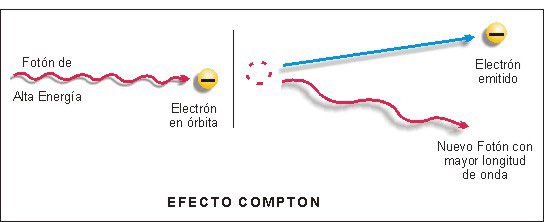
\includegraphics[scale=0.75]{Compton.jpeg}
		 	\caption{Efecto Compton}
		\end{figure}		
		
			\subsection{Propiedades corpusculares de la radiación}
			
				En su artículo "teoría cuántica de la dispersión de rayos X por elementos ligeros" Compton escribió: "La presente teoría depende esencialmente de la suposición de que cada electrón que efectivo en la dispersión, dispersa un quantum completo (fotón). También involucra la hipótesis de que un quantum de radiación se recibe desde direcciones definidas y se dispersa en direcciones definidas. El soporte experimental de la teoría indica de manera muy convincente que un quantum de radiación lleva consigo su impulso y su energía".
				
			\subsection{Longitud de onda de Compton}
			
				De la deducción de la ecuación de Compton se obtiene \boxed{\lambda_c=\frac{h}{m_0c}=2.43x10^{-12}m=0.0243 \AA}\\
				Llamada \textbf{Longitud de onda de Compton}
			
		\section{Modelo de Bohr del átomo de Hidrógeno}
			\subsection{Postulados}
			
				\begin{enumerate}
					\item Un electrón en un átmo se mueve en una \textbf{órbita circular} alrededor del núcleo bajo la influencia de la atracción de Coulomb entre el electrón y el núcleo, sujetándose a las leyes de la mecánica clásica.
					\item Para un electrón sólo es posible moverse en una órtiba para la cual su \textbf{impulso angular orbital $L$ está cuantizado}. $L=n \hbar$ para $n=1,2,3\ldots$
					\item El electrón \textbf{no emite radiación} electromagnética a pesar de acelerarse constantemente en su movimiento circular. La energía total $E$ permanece constante
					\item Se emite radiación electromagnética si un electrón inicialmente en una órbita de energía $E_i$, cambia de manera discontinua para moverse en una órbita de energía $E_f$. La frecuencia de la radiación emitida será $\upsilon=\frac{E_i-E_f}{h}$
				\end{enumerate}							
			
			\subsection{Niveles energéticos}		
			
				Considerando un átomo que consiste de un núcleo de carga $+Ze$ y masa $M$ y un solo electrón de carga $-e$ y masa $m$, para un átomo de hidrógeno neutro $Z=1$. La condición de estabilidad mecánica del electrón implica:
				
				\begin{center}
					$\displaystyle F_{coulomb}=\frac{1}{4\pi \epsilon_0}\frac{Ze^2}{r^2}=m\frac{v^2}{r}=ma_c$\\		
			
					Como $L=n\hbar=mvr$, se obtiene \boxed{r=4\pi \epsilon_0 \frac{n^2\hbar^2}{mZe^2}} y \boxed{v=\frac{n\hbar}{mr}=\frac{1}{4\pi \epsilon_0}\frac{Ze^2}{n\hbar}}
				\end{center}
			
			Las velocidades y los radios de las órbitas están cuantizados.\\
			
			Se puede calcular la energía potencial cuando el electrón atómico que se mueve en una de las órbitas permitidas. Definiendo el cero de la energía potencial en el infinto. Además de su energía potencial.\\
			
			\begin{minipage}[t]{0.5\textwidth}
				$\displaystyle V=-\int_r^\infty F_{coulomb}dr=-\int_r^\infty \frac{Ze^2}{4\pi \epsilon_0 r^2}dr=-\frac{Ze^2}{4\pi \epsilon_0r}$
			\end{minipage}
			\begin{minipage}[t]{0.25\textwidth}
				$\displaystyle K=\frac{1}{2}mv^2=\frac{Ze^2}{4\pi \epsilon_0 2r}$
			\end{minipage}
			\begin{center}
				$\displaystyle E=K+V=-\frac{Ze^2}{4\pi \epsilon_0 2r}=-K \Rightarrow$\boxed{\displaystyle E=-\frac{mZ^2e^4}{(4\pi \epsilon_0)^2 2 \hbar^2}\frac{1}{n^2}} con $n=1,2,3 \ldots$
			\end{center}
			
				\textit{La cuantización del impulso angular orbital del electrón conduce a una cuantización de su energía total.}			
			
			\subsection{Espectro del Hidrógeno}	
			
				La radiación electromagnética emitida por átomos libres se concentra en un número de longitudes de onda discretas. Cada átomo posee su propio espectro característico, fundamento de la espectroscopía en el análisis químico.\\
				
				El espectro del hidrógeno es relativamente simple. El espaciamiento entre líneas del espectro, en longitudes de onda, decrece continuamente conforme decrece la longitud de onda de las líneas, de manera que la serie de líneas converge a la llamada límite de la serie en $3656.6 \AA$. La regularidad del espectro del hidrógeno llevó a buscar diversas fórmulas empíricas, entre ellas la serie de Balmer:
				
				\begin{center}
				$\displaystyle \lambda=3646\frac{n^2}{n^2-4}$ (Predice las primeras nueve líneas de la serie)
				\end{center}
			
			\begin{figure}[H]
				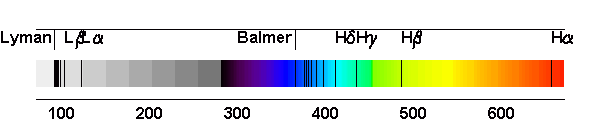
\includegraphics[scale=0.75]{EspectroH.png}
				\caption{Espectro del Hidrógeno}
			\end{figure}
			
			\subsection{Constante de Rydberg}
			
				Rydberg encontró mas conveniente trabajar con el recíproco de la longitud de onda de las líneas. En términos del recíproco de la longitud de onda en la fórmula de Balmer, se puede escribir:
				
				\begin{center}
					$\displaystyle \kappa=1/\lambda=R_H(\frac{1}{2^2}-\frac{1}{n^2})$ con $n=3,4,5,\ldots$		
				\end{center}
			
			Donde $R_H$ es la llamada \textbf{constante de Rydberg del Hidrógeno}, cuyo valor es $10967757 \pm 1.2 m^{-1}$			
			
			\subsection{Fallas en la teoría de Bohr}
			
				\begin{enumerate}
					\item Aunque establece la manera de calcular las energías de los estados permitidos para ciertos sistemas y la frecuencia de los fotones emitidos o absorbidos cuando un sistema sufre una transición entre estados permitidos, no establece la manera de calcular las velocidades a las cuales ocurren tales transiciones, las intensidades de las líneas espectrales ni tampoco cuáles transiciones realmente se observan y cuáles no.
					\item La teoría solamente tiene éxito para átomos monoelectrónicos, aproximadamente para los elementos alcalinos, pero falla incluso para el átomo de $He$ neutro, el cual contiene sólo dos electrones.
				\end{enumerate}							
			
		\section{Difracción e interferencia de ondas electromagnéticas}
			\subsection{Interpretación probabilística}
			\subsection{Dualidad onda-corpúsculo (fotón)}
		\section{Difracción e interferencia de partículas materiales}
			\subsection{Propiedades ondulatorias}
			\subsection{Funciones de amplitud de onda y densidad de probabilidad}
			\subsection{Experimento de Davidson-Germer de difracción de electrones} 
		\section{Longitud de onda de De Broglie}
			
			De Broglie propuso que el comportamiento dual de la radiación debería ser igualmente aplicable a la materia. Así como el fotón tiene asociado una onda de luz que gobierna su movimiento, una partícula de materia tiene asociada una \textbf{onda de materia} que gobierna su movimiento.\\
			
			Tanto para la materia como para la radiación, la energía total E de un ente se relaciona con la frecuencia $\upsilon$ de la onda asociada a su movimiento por medio de la ecuación $E=h\upsilon$ y el impulso $p$ del ente se relaciona con la longitud de onda $\lambda$ de la onda asociada por la ecuación $p=h/\lambda$.\\
			
			Los conceptos corpusculares energía $E$, e impulso $p$, se relacionan con los conceptos ondulatorios frecuencia $\upsilon$ y longitud de onda $\lambda$ a través de la constante de Planck $h$.
			
			La \textbf{relación de De Broglie}: \boxed{\lambda=h/p} precide la \textbf{longitud de onda de De Broglie} de una onda de materia asociada con el movimiento de una partícula material de impulso $p$.
		
			\subsection{Dualidad Onda-Partícula}
			
				La relación carga-masa del electrón sugiere un modelo corpuscular, sin embargo, la difracción de electrones sugiere un modelo ondulatorio. En una medición dada, se debe aplicar un solo modelo. Cuando una partícula es detectada mediante algún tipo de interacción, actúa como partícula, en el sentido de que está localizada; cuando está en movimiento, actúa como onda, e el sentido de que se observan fenómenos de interferencia y no está localizada.\\
				
				Bohr enunció el \textbf{principio de complementaridad}, que dice que los modelos corpuscular y ondulatorio son complementarios, pero que cuál debe utilizarse lo determina la naturaleza del experimento.\\
				
				La conexión entre ambos modelos se encuentra en una interpretación probabilística de la dualidad onda-partícula, asociando al movimiento una función de onda.\\
			
		\section{Principio de incerteza de Heisemberg}
				
			Establece que no se puede determinar la posición y el impulso de la materia o la radiación, en el mismo instante, no más exactamente que lo permitido por $\Delta p_x \Delta x \geq \hbar/2$(y las otras componentes).La restricción no está en la precisión con la que se pueda medir $x$ o $p_x$, sino en el producto de sus incertezas en una medida simultánea de ambas.\\
			
			La segunda	parte del principio de incertidumbre está relacionada con medidas de la energía $E$ y el tiempo $t$ necesarios para medir, definido por la ecuación: $\Delta E \Delta t \geq \hbar/2$\\
			
			En lugar de hacer predicciones deterministas sólo se puede enunciar los resultados más probables de una observación. Como el hecho de observar un sistema lo perturba de modo no completamente predecible, la observación cambia el movimiento anterior del sistema a un estado de movimiento nuevo que no puede ser conocido completamente.
			
\nopagebreak
	\chapter{Mecánica cuántica}
		\section{Ecuación de Schrödinger (completa)}	
		
			La teoría específica las leyes del movimiento ondulatorio que obedecen las partículas de cualquier sistema microscópico. Lo cual se hace especificando, para cada sistema, la ecuación que controla el comportamiento de la función de onda y especificando también la conexión entre el comportamiento de la función de onda y el comportamiento de la partícula.\\
			
			La ecuación de Schrödinger es: \boxed{\displaystyle -\frac{\hbar^2}{2m}\nabla^2 \Psi(x,t)+V(x,t)\Psi(x,t)=i\hbar\frac{\partial \psi(x,t)}{\Psi t}}
			
			\subsection{Argumentos para postular una función de onda para describir el movimiento de partículas}
			
			\begin{enumerate}
				\item Deberá ser coincidente con los postulados de De Broglie-Einstein $\lambda=h/p$ y $\upsilon=E/h$
				\item Deberá ser coincidente con la ecuación $E=\frac{p^2}{2m}+V$ que relaciona la energía total $E$ de una partícula de masa m con su energía cinética y potencial.
				\item Deberá ser lineal en $\Psi(x,t)$ de manera tal de poder sumar funciones de onda para producir las interferencias constructivas y destructivas de las ondas.
				\item La energía potencial V generalmente es una función de $x$ y posiblemente de $t$. Sin embargo si $V(x,t)=V_0$ entonces la fuerza que actúa sobre la partícula será nula y será constante el impulso $p$ y la energía $E$, lo cuál implica que la función de onda tendrá frecuencia $\upsilon$ y longitud de onda $\lambda$ constantes.
			\end{enumerate}
			
			\subsection{Significado físico de la función de onda}
			
				Puesto que una función de onda  $\displaystyle \Psi(x,t)$ de la mecánica cuántica especifíca simultáneamente dos funciones reales, su parte real y su parte imaginaria, se hace evidente que no se debería dar a las funciones de onda una existencia física en el mismo sentido que la tienen las ondas en el agua.\\
				
				Las funciones de onda son dispositivos computacionales que solamente tienen significado en el contexto de la teoría de Schrödinger de la cual forman parte. Contiene toda la información que el principio de incertidumbre permite conocer acerca de la partícula asociada.\\		
			
				La conexión básica entre las propiedades de la función de onda $\displaystyle \Psi(x,t)$ y el comportamiento de la partícula asociada  está expresada en términos de la \textbf{densidad de probabilidad} $P(x,t)$, probabilidad por unidad de longitud del eje x de encontrar a la partícula en la vecindad de la coordenada $x$ al tiempo $t$.
				
				\begin{center}
				\boxed{\displaystyle P(x,t)=\Psi(x,t)^*\Psi(x,t)}
				\end{center}
							
				Si en el instante $t$ se realiza una medición para localizar a la partícula asociada con la función de onda $\displaystyle \Psi(x,t)$, entonces la probabilidad $P(x,t)dx$ de encontrar a la partícula en una coordenada entre $x$ y $x+dx$ es igual a $\displaystyle \Psi(x,t)^*\Psi(x,t)dx$\\
		
				Al trabajar con densidad de probabilidad es necesario que la función de onda se encuentre normalizada.\\		
			
		\section{Ecuación de Schödinger independiente del tiempo}
			
			Aplicando el método de separación de variables, se puede escribir $\Psi(x,t)=\psi(x)\varphi(t)$, siempre que la energía potencial no dependa explícitamente del tiempo $t$, de modo tal de tener $V(x)$.\\
			
			\begin{center}
			Esto lleva a $\displaystyle \frac{1}{\psi(x)}\left[-\frac{\hbar^2}{2m}\frac{d^2\psi(x)}{dx^2}+V(x)\psi(x)\right]=i\hbar\frac{1}{\varphi(t)}\frac{d\varphi(t)}{dt}=G$
			\end{center}
		
			Siendo que $G$ no puede depender de la posición ni del tiempo, entonces debe ser una constante de separación de ambas variables. Logrando desacoplar en problema.\\
		
			La ecuación diferencial de la variable temporal se puede escribir: $\displaystyle \frac{d\varphi(t)}{dt}=-\frac{iG}{\hbar}\varphi(t) \rightarrow \varphi(t)=e^{-i\frac{E}{\hbar}t}$\\
		
			Utilizando $G=E$ debido a que según el postulado de De Broglie-Einstein, la frecuencia es $\upsilon=E/h$\\
			
			Resolviendo la ecuación diferencial en su variable espacial $\displaystyle -\frac{\hbar^2}{2m}\frac{d^2\psi(x)}{dx^2}+V(x)\psi(x)=E\psi(x)$\\
			
			\begin{center}
			Finalmente se llega a \boxed{\displaystyle \Psi(x,t)=\psi(x)e^{-i\frac{E}{\hbar}t}}
			\end{center}
		
			\subsection{Condiciones de frontera}
						
				\begin{minipage}[t]{0.5\textwidth}
					\begin{itemize}
						\item $\psi(x)$ debe ser finita
						\item $\psi(x)$ debe ser monovaluada
						\item $\psi(x)$ debe ser continua\\
					\end{itemize}
				\end{minipage}
				\begin{minipage}[t]{0.5\textwidth}
					\begin{itemize}
						\item $d\psi(x)/dx$ debe ser finita
						\item $d\psi(x)/dx$ debe ser monovaluada
						\item $d\psi(x)/dx$ debe ser continua
					\end{itemize}
				\end{minipage}
			
		\section{Aplicaciones en una dimensión}
				\subsection{Partícula libre}
				
					Bajo la acción de $V(x)=0$ la partícula se ve afectada por una fuerza $F=-dV(x)/dx=0$. Se eligió el cero, pero puede emplearse cualquier constante, no se pierde generalidad, la fuerza seguirá siendo nula.\\
					
					La mecánica clásica establece que una partícula libre estará en reposo o en movimiento, pero con impulso $p$ constante y por lo tanto energía total $E$ constante y mayor a cero.\\
					
					Como el potencial no depende del tiempo, se aplica el método de separación de variables: 
					
					\begin{center}
					$\Psi(x,t)=\psi(x)\varphi(t) \Rightarrow \displaystyle \Psi(x,t)=\psi(x)e^{-i\frac{E}{\hbar}t}$\\
					\end{center}
					\begin{center}
					$\displaystyle  -\frac{\hbar^2}{2m}\frac{d^2\psi(x)}{dx^2}+\underbrace{V(x)}_{0}\psi(x)=E\psi(x)$\\					
					\end{center}				
					\begin{center}
					$\displaystyle  -\frac{\hbar^2}{2m}\frac{d^2\psi(x)}{dx^2}=E\psi(x) \Rightarrow \frac{d^2\psi(x)}{dx^2}=-\underbrace{\frac{2mE}{\hbar^2}}_{k^2}\psi(x)=-k^2\psi(x)$\\					
					\end{center}		
					\begin{center}
					\boxed{\displaystyle \psi(x)=Ae^{ikx}+Be^{-ikx} \text{ con } k=\frac{\sqrt{2mE}}{\hbar}}
					\end{center}
					
					Si se analiza el caso de una onda que viaja en la dirección que $x$ crece ($B=0$), la partícula cuyo movimiento está descrito por estas funciones también viaja en dicha dirección. Facilmente verificable calculando el valor medio de su impulso lineal utilizando su operador $\hat{p}=-i\hbar\frac{\partial}{\partial x}$
					
					 \begin{center}
					 $\displaystyle \overline{p}=\int_{-\infty}^{\infty}\Psi(x,t)^*\hat{p}\Psi(x,t)dx=\int_{-\infty}^{\infty}\Psi(x,t)^*(-i\hbar\frac{\partial}{\partial x}Ae^{ikx}e^{-i\frac{E}{\hbar}t})dx=\int_{-\infty}^{\infty}\Psi(x,t)^*(\sqrt{2mE})\Psi(x,t)dx \Rightarrow$\\
					 \end{center}
					 \begin{center}
					 $\displaystyle \sqrt{2mE}\int_{-\infty}^{\infty}\Psi(x,t)^*\Psi(x,t)dx=\sqrt{2mE}\underbrace{\int_{-\infty}^{\infty}\psi(x,t)^*\psi(x,t)\underbrace{e^{-i\frac{E}{\hbar}t}e^{i\frac{E}{\hbar}t}}_1dx}_{1 \text{ Por normalización}}=+\sqrt{2mE}$
					 \end{center}
				
					Que es exactamente el impulso que debería tener una partícula libre que se mueve en la dirección en la que crece $x$ con una energía total $E$. Análogamente para una partícula que se mueve en la dirección que $x$ decrece ($A=0$) se lleva a $\hat{p}=-\sqrt{2mE}$\\
				
					La coordenada $x$ es completamente desconocida debido a que las amplitudes de las ondas son las mismas en todas las regiones del eje $x$.Considerando en una sola dirección\\
					
					\begin{center}
					$\Psi(x,t)^*\Psi(x,t)=A^*e^{-ikx}Ae^{ikx}e^{i\frac{E}{\hbar}t}e^{-i\frac{E}{\hbar}t}=A^*A \text{ (Independiente de x)}$\\
					\end{center}
				
					La partícula se encontrará igualmente en cualquier punto y \boxed{\Delta x=\infty}, por el principio de incertidumbre se tiene $\Delta p \Delta x \geq \hbar/2 \Rightarrow$ \boxed{\Delta p=0}\\					
				
				\subsection{Escalón de potencial}		
				
				Se define el potencial escalón como $\displaystyle V(x)=\begin{Bmatrix} V_0 & \mbox{ si }& x>0 \\ 0 & \mbox{si}& x<0\end{Bmatrix}$
				
				\begin{figure}[H]
					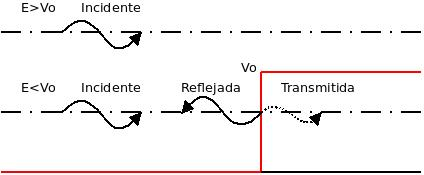
\includegraphics[scale=1]{Escalon.jpeg}
					\caption{Potencial escalón}
				\end{figure}
				
				\begin{minipage}[t]{0.5\textwidth}
					\begin{center}
						\textbf{$E<V_0$}
					\end{center}
					\begin{center}
						$\Downarrow$
					\end{center}
					\begin{center}
						$\displaystyle -\frac{\hbar^2}{2m}\frac{d^2\psi(x)}{dx^2}=E\psi(x) \text{ si } x<0$
					\end{center}
					\begin{center}
						$\displaystyle -\frac{\hbar^2}{2m}\frac{d^2\psi(x)}{dx^2}+V_0\psi(x)=E\psi(x) \text{ si } x>0$
					\end{center}
					\begin{center}
						$\Downarrow$
					\end{center}
					\begin{center}
						$\displaystyle \psi(x)=Ae^{ik_1x}+Be^{-ik_1x} \text{ con } k_1=\frac{\sqrt{2mE}}{\hbar} \text{ si } x<0$
					\end{center}
					\begin{center}
						$\displaystyle \psi(x)=Ce^{k_2x}+De^{-k_2x} \text{ con } k_2=\frac{\sqrt{2m(V_0-E)}}{\hbar} \text{ si } x>0$
					\end{center}
					\begin{center}
						$\Downarrow$
					\end{center}
				\end{minipage}
				\begin{minipage}[t]{0.5\textwidth}
					\begin{center}
						\textbf{$E>V_0$}
					\end{center}
					\begin{center}
						$\Downarrow$
					\end{center}
					\begin{center}
						$\displaystyle -\frac{\hbar^2}{2m}\frac{d^2\psi(x)}{dx^2}=E\psi(x) \text{ si } x<0$
					\end{center}
					\begin{center}
						$\displaystyle -\frac{\hbar^2}{2m}\frac{d^2\psi(x)}{dx^2}+V_0\psi(x)=E\psi(x) \text{ si } x>0$
					\end{center}
					\begin{center}
						$\Downarrow$
					\end{center}
					\begin{center}
						$\displaystyle \psi(x)=Ae^{ik_1x}+Be^{-ik_1x} \text{ con } k_1=\frac{\sqrt{2mE}}{\hbar} \text{ si } x<0$
					\end{center}
					\begin{center}
						$\displaystyle \psi(x)=Ce^{ik_2x}+De^{-ik_2x} \text{ con } k_2=\frac{\sqrt{2m(E-V_0)}}{\hbar} \text{ si } x>0$
					\end{center}
					\begin{center}
						$\Downarrow$
					\end{center}
				\end{minipage}
				
				\vspace{3cm}

				\begin{minipage}[t]{0.5\textwidth}
					\begin{center}
						$\psi(x)$ debe ser finita\\
						por eso se impone $C=0$
					\end{center}
					\begin{center}
						$\Downarrow$
					\end{center}
					\begin{center}
						$\displaystyle D(e^{-k_2x})_{x=0}=A(e^{ik_1x})_{x=0}+B(e^{-ik_1x})_{x=0}$
					\end{center}
					\begin{center}
						$\displaystyle \frac{d(De^{-k_2x})}{dx}_{x=0}=\frac{d(Ae^{ik_1x})}{dx}_{x=0}+\frac{d(B(e^{-ik_1x})}{dx}_{x=0}$
					\end{center}
					\begin{center}
						$\Downarrow$
					\end{center}
					\begin{center}
						\begin{minipage}[t]{0.3\textwidth}
							\begin{center}
								$D=A+B \Rightarrow$
							\end{center}
							\begin{center}
								$\displaystyle i\frac{k_2}{k_1}D=A-B \Rightarrow$
							\end{center}					
						\end{minipage}	
						\begin{minipage}[t]{0.3\textwidth}
							\begin{center}
								$\displaystyle A=\frac{D}{2}(1+i\frac{k_2}{k_1})$
							\end{center}
							\begin{center}
								$\displaystyle B=\frac{D}{2}(1-i\frac{k_2}{k_1})$
							\end{center}
						\end{minipage}	
					\end{center}			
					\begin{center}
						$\Downarrow$
					\end{center}
					\begin{center}
						$\displaystyle \psi(x)=\frac{D}{2}(1+i\frac{k_2}{k_1})e^{ik_1x}+\frac{D}{2}(1-i\frac{k_2}{k_1})e^{-ik_1x} \text{ si } x<0$
					\end{center}
					\begin{center}
						$\displaystyle \psi(x)=De^{-k_2x} \text{ con } k_2=\frac{\sqrt{2m(V_0-E)}}{\hbar} \text{ si } x>0$
					\end{center}
					\begin{center}
						$\Downarrow$
					\end{center}
					\begin{center}
						Coeficiente de Reflexión:\\
						Probabilidad Reflejada/Probabilidad Incidente
					\end{center}
					 \begin{center}
						$\displaystyle R=\frac{v_1B^*B}{v_1A^*A}=1$
					\end{center}
					 \begin{center}
						Coeficiente de Transmisión:\\
						Probabilidad Transmitida/Probabilidad Incidente
					\end{center}
					 \begin{center}
						$\displaystyle T=\frac{v_2C^*C}{v_1A^*A}=0$
					\end{center}
				\end{minipage}
				\begin{minipage}[t]{0.5\textwidth}
					\begin{center}
						Sin potencial que provoque reflexión\\
						por eso se impone $D=0$
					\end{center}
					\begin{center}
						$\Downarrow$
					\end{center}
					\begin{center}
						$\displaystyle A(e^{ik_1x})_{x=0}+B(e^{-ik_1x})_{x=0}=C(e^{ik_2x})_{x=0}$
					\end{center}
					\begin{center}
						$\displaystyle \frac{d(Ae^{ik_1x})}{dx}_{x=0}+\frac{d(Be^{-ik_1x})}{dx}_{x=0}=\frac{d(C(e^{ik_2x})}{dx}_{x=0}$
					\end{center}
					\begin{center}
						$\Downarrow$
					\end{center}
					\begin{center}
						\begin{minipage}[t]{0.3\textwidth}
							\begin{center}
								$A+B=C \Rightarrow$
							\end{center}
							\begin{center}
								$\displaystyle \frac{k_1}{k_2}C=A-B \Rightarrow$
							\end{center}					
						\end{minipage}	
						\begin{minipage}[t]{0.3\textwidth}
							\begin{center}
								$\displaystyle B=\frac{k_1-k_2}{k_1+k_2}A$
							\end{center}
							\begin{center}
								$\displaystyle C=\frac{2k_1}{k_1+k_2}A$
							\end{center}
						\end{minipage}	
					\end{center}				
					\begin{center}
						$\Downarrow$
					\end{center}
					\begin{center}
						$\displaystyle \psi(x)=Ae^{ik_1x}+\frac{k_1-k_2}{k_1+k_2}Ae^{-ik_1x} \text{ si } x<0$
					\end{center}
					\begin{center}
						$\displaystyle \psi(x)=\frac{2k_1}{k_1+k_2}Ae^{ik_2x} \text{ si } x>0$
					\end{center}
					\begin{center}
						$\Downarrow$
					\end{center}
					\begin{center}
						Coeficiente de Reflexión:\\
						Probabilidad Reflejada/Probabilidad Incidente
					\end{center}
					\begin{center}
						$\displaystyle R=\frac{v_1B^*B}{v_1A^*A}=\left(\frac{k_1-k_2}{k_1+k_2}\right)^2$
					\end{center}
					\begin{center}
						Coeficiente de Transmisión:\\
						Probabilidad Transmitida/Probabilidad Incidente
					\end{center}
					\begin{center}
						$\displaystyle T=\frac{v_2C^*C}{v_1A^*A}=\frac{v_2}{v_1}\left(\frac{2k_1}{k_1+k_2}\right)^2$
					\end{center}
				\end{minipage}
				
				\vspace{1cm}
				
				\begin{center}
				En ambos casos $\displaystyle v_1=\frac{p_1}{m}=\frac{\hbar k_1}{m}$ y $\displaystyle v_2=\frac{p_2}{m}=\frac{\hbar k_2}{m}$ y se cumple $R+T=1$. 
				\end{center}
						
				Se deben interpretar los coeficientes de transmisión y reflexión como un flujo de probabilidades, la probabilidad por segundo de encontrar una partícula cruzando algún punto de referencia en una dirección particular.$R=1$ y $T=0$ implica que la probabilidad de que la partícula sea reflejada es absoluta, pero eso no quiere decir que no pueda transmitirse, en contradicción con la teoría clásica. En el segundo caso, se pone de manifiesto que existe una probabilidad de que la partícula sea reflejada, aún cuando la energía es superior a la del escalón del potencial.
					
				\subsection{Pozo de potencial infinito}
				
				Se define al potencial infinito como: $\displaystyle V(x)=\begin{Bmatrix} \infty & \mbox{ si }& x>|\frac{a}{2}| \\ 0 & \mbox{si}& x<|\frac{a}{2}|\end{Bmatrix}$\\
				
				Tiene la característica de ligar una partícula con cualquier energía total finita $E \geq 0$, pero solamente son permitidos ciertos eigenvalores discretos de $E$\\
				
				\begin{figure}[H]
					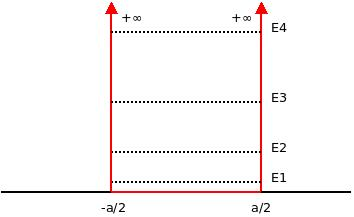
\includegraphics[scale=1]{PozoInfinito.jpeg}
					\caption{Potencial de pozo cuadrado infinito}
				\end{figure}				
				
				La solución general a la ecuación 	de Schrödinger independiente del tiempo para la región interna de un pozo cuadrado infinito se puede escribir como una onda estacionaria:\\
				
				\begin{center}
					$\displaystyle \psi(x)=Ae^{ikx}+Be^{-ikx} \text{ con } k=\frac{\sqrt{2mE}}{\hbar} \text{ Con la condición } \psi(x=\pm a/2)=0$
				\end{center}
				\begin{center}
					$\displaystyle \psi(x)=Ae^{ika/2}+Be^{-ika/2}=0 \text{  y  }  \psi(x)=Ae^{-ika/2}+Be^{ika/2}=0$
				\end{center}
				\begin{center}
					Sumando ambos: $\displaystyle 2(A+B)\cos(ka/2)=0$
				\end{center}
				\begin{center}
					Restando ambos: $\displaystyle 2i(A-B)\sin(ka/2)=0$
				\end{center}
				\begin{center}
					$\Downarrow$
				\end{center}
				
				\begin{minipage}[t]{0.4\textwidth}				
					\begin{center}
						$\displaystyle k_n=\frac{n\pi}{a} \text{ con } n=1,3,5,\ldots$\\
						y\\
						$A=B$
					\end{center}
				\end{minipage}
				\begin{minipage}[t]{0.4\textwidth}				
					\begin{center}
						$\displaystyle k_n=\frac{n\pi}{a} \text{ con } n=2,4,6,\ldots$\\
						y\\
						$A=-B$
					\end{center}
				\end{minipage}
				
				\begin{center}
					$\Downarrow$
				\end{center}
				
				\begin{center}
				$\displaystyle \psi_n(x)=\begin{Bmatrix} 2A\cos(k_nx)  & \mbox{ si }& x>|\frac{a}{2}| \mbox{ y } n=1,3,5,\ldots \\ -2iB\sin(k_nx) & \mbox{si}& x<|\frac{a}{2}| \mbox{ y } n=2,4,6,\ldots \end{Bmatrix}$
				\end{center}
				
				Utilizando la expresión del número de onda que se encontró inicialmente y la que se tiene en la solución general, se llega a la \textbf{cuantización de la energía total} para una partícula ligada al pozo de potencial infinito.\\
				
				$\displaystyle k_n=\frac{n\pi}{a}=\frac{\sqrt{2mE}}{\hbar} \Rightarrow$ \boxed{\displaystyle E_n=\frac{n^2\pi^2\hbar^2}{2ma^2}=\left(\frac{\pi\hbar}{a}\right)^2\frac{n^2}{2m}} La energía del primer eigenvalor es la \textbf{energía del punto cero}, la mas baja posible que puede tener una partícula ligada en la región del pozo de potencial infinito. No puede tener energía total cero, debido a que se conoce la coordenada $x$ dentro de una incertidumbre de $\Delta x \simeq a$, en consecuencia la incertidumbre de su impulso lineal deberá ser al menos $\displaystyle \Delta p\simeq \frac{\hbar}{2\Delta x}=\frac{\hbar}{2a}$. El principio de incertidumbre no puede permitir que la partícula esté ligada por el potencial con energía total cero ya que esto significaría que la incertidumbre en el impulso debería ser igual a cero.
				
				\subsection{Pozo de potencial finito}		
				
				Se define al potencial finito como: $\displaystyle V(x)=\begin{Bmatrix} V_0 & \mbox{ si }& x>|\frac{a}{2}| \\ 0 & \mbox{si}& x<|\frac{a}{2}|\end{Bmatrix}$\\
								
				Tiene la característica de ligar una partícula con cualquier energía total finita $0 \leq E \leq V_0$, con ciertos valores permitidos. Por encima de dicha energía se tienen valores continuos.\\
				
				\begin{figure}[H]
					\begin{center}
						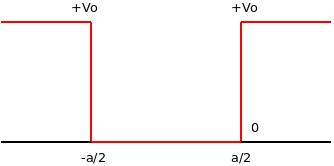
\includegraphics[scale=1]{PozoFinito.jpeg}
						\caption{Potencial de pozo cuadrado finito}
					\end{center}
				\end{figure}				
				
				Se busca solución a la ecuación de Schrödinger independiente del tiempo para una partícula libre con energía menor a $V_0$ confinada al pozo de potencial.\\
				
				\begin{center}
					$\displaystyle \psi(x)=Ae^{k_1x}+Be^{-k_1x} \text{ si } x<-a/2 \text{ con } k_1=\frac{\sqrt{2m(V_0-E)}}{\hbar}$				
				\end{center}
				\begin{center}
					$\displaystyle \psi(x)=Ce^{ik_2x}+De^{-ik_2x} \text{ si } -a/2<x<a/2 \text{ con } k_2=\frac{\sqrt{2mE}}{\hbar}$
				\end{center}
				\begin{center}
					$\displaystyle \psi(x)=Fe^{k_1x}+Ge^{-k_1x} \text{ si } x>a/2 \text{ con } k_1=\frac{\sqrt{2m(V_0-E)}}{\hbar}$
				\end{center}
				\begin{center}
					$\Downarrow$
				\end{center}
				
				Las eigenfunciones deben permanecer finitas para toda $x$, por lo que $B=0$ y $F=0$ y deben ser continuas junto a sus primeras derivadas, en $x=\pm a/2$
				
				\begin{center}
					$\Downarrow$
				\end{center}
				\begin{center}
					$\displaystyle Ae^{-k_1a/2}=Ce^{-ik_2a/2}+De^{ik_2a/2}$	\hspace{1cm}	$\displaystyle k_1Ae^{-k_1a/2}=iCk_2e^{-ik_2a/2}-iDk_2e^{ik_2a/2}$		
				\end{center}
				\begin{center}
					$\displaystyle Ce^{ik_2a/2}+De^{-ik_2a/2}=Ge^{-k_1a/2}$	\hspace{1cm} $\displaystyle iCk_2e^{ik_2a/2}-iDk_2e^{-ik_2a/2}=-k_1Ge^{-k_1a/2}$		
				\end{center}
				
				\begin{center}
					$\Downarrow$
				\end{center}
				 
				\begin{center}
					$\displaystyle Ae^{-k_1a/2}=Ce^{-ik_2a/2}+De^{ik_2a/2}$	\hspace{1cm}	$\displaystyle -i\frac{k_1}{k_2}Ae^{-k_1a/2}=Ce^{-ik_2a/2}-De^{ik_2a/2}$		
				\end{center}
				\begin{center}
					$\displaystyle Ce^{ik_2a/2}+De^{-ik_2a/2}=Ge^{-k_1a/2}$	\hspace{1cm} $\displaystyle Ce^{ik_2a/2}-De^{-ik_2a/2}=i\frac{k_1}{k_2}Ge^{-k_1a/2}$		
				\end{center}
				
				\begin{center}
					$\Downarrow$
				\end{center}
				
				\begin{center}
					$\displaystyle C=(1-i\frac{k_1}{k_2})\frac{A}{2}e^{(ik_2-k_1)a/2}$	\hspace{1cm}	$\displaystyle D=(1+i\frac{k_1}{k_2})\frac{A}{2}e^{-(ik_2+k_1)a/2}$		
				\end{center}
				\begin{center}
					$\displaystyle C=(1+i\frac{k_1}{k_2})\frac{G}{2}e^{-(ik_2+k_1)a/2}$	\hspace{1cm} $\displaystyle D=(1-i\frac{k_1}{k_2})\frac{G}{2}e^{(ik_2-k_1)a/2}$		
				\end{center}
				
				\begin{center}
					$\Downarrow$
				\end{center}
				
				\begin{center}
					$\displaystyle (1+i\frac{k_1}{k_2})\frac{G}{2}e^{-(ik_2+k_1)a/2}=(1-i\frac{k_1}{k_2})\frac{A}{2}e^{(ik_2-k_1)a/2}$
				\end{center}
				\begin{center}
					 $\displaystyle (1+i\frac{k_1}{k_2})\frac{A}{2}e^{-(ik_2+k_1)a/2}=(1-i\frac{k_1}{k_2})\frac{G}{2}e^{(ik_2-k_1)a/2}$		
				\end{center}
				
				\begin{center}
					$\Downarrow$
				\end{center}
				
				\begin{center}
					$\displaystyle \frac{G}{A}=\frac{A}{G} \Rightarrow A=-G \text{ o } A=G$
				\end{center}
		
		Si $A=-G \Rightarrow$:
		
				\begin{center}
					$\displaystyle \frac{ik_1+k_2}{ik_1-k_2}=e^{ik_2a}$
				\end{center}
				
				\begin{center}
					$\displaystyle \psi(x)=-Ge^{k_1x} \text{ si } x<-a/2 \text{ con } k_1=\frac{\sqrt{2m(V_0-E)}}{\hbar}$				
				\end{center}
				\begin{center}
					$\displaystyle \psi(x)=(ik_1+k_2)G \sinh \left(\frac{k_1a}{2}+ik_2(x-\frac{a}{2})\right) \text{ si } -a/2<x<a/2 \text{ con } k_2=\frac{\sqrt{2mE}}{\hbar}$
				\end{center}
				\begin{center}
					$\displaystyle \psi(x)=Ge^{-k_1x} \text{ si } x>a/2 \text{ con } k_1=\frac{\sqrt{2m(V_0-E)}}{\hbar}$
				\end{center}
				
				\begin{center}
					$\displaystyle \frac{i\sqrt{V_0-E}+\sqrt{E}}{i\sqrt{V_0-E}-\sqrt{E}}=e^{i\frac{\sqrt{2mE}}{\hbar}a}$
				\end{center}
				\begin{center}
					Los valores de $E$ que cumplan la ecuación serán los de energía permitida siempre que $E \leq V_0$
				\end{center}				
			
		Si $A=G \Rightarrow$:
		
				\begin{center}
					$\displaystyle \frac{ik_1+k_2}{-ik_1+k_2}=e^{ik_2a}$
				\end{center}
				
				\begin{center}
					$\displaystyle \psi(x)=Ge^{k_1x} \text{ si } x<-a/2 \text{ con } k_1=\frac{\sqrt{2m(V_0-E)}}{\hbar}$				
				\end{center}
				\begin{center}
					$\displaystyle \psi(x)=(ik_1+k_2)G \sinh \left(\frac{k_1a}{2}+ik_2(x-\frac{a}{2})\right) \text{ si } -a/2<x<a/2 \text{ con } k_2=\frac{\sqrt{2mE}}{\hbar}$
				\end{center}
				\begin{center}
					$\displaystyle \psi(x)=Ge^{-k_1x} \text{ si } x>a/2 \text{ con } k_1=\frac{\sqrt{2m(V_0-E)}}{\hbar}$
				\end{center}
				
				\begin{center}
					$\displaystyle -\frac{i\sqrt{V_0-E}+\sqrt{E}}{i\sqrt{V_0-E}-\sqrt{E}}=e^{i\frac{\sqrt{2mE}}{\hbar}a}$
				\end{center}
				\begin{center}
					Los valores de $E$ que cumplan la ecuación serán los de energía permitida siempre que $E \leq V_0$
				\end{center}	
				
				\subsection{Barrera de potencial}		
				
					Se define la barrera de potencial como: $\displaystyle V(x)=\begin{Bmatrix} V_0 & \mbox{ si }& 0<x<a \\ 0 & \mbox{si}& 0<x \text{ o } x>a \end{Bmatrix}$\\
				
				\begin{figure}[H]
					\begin{center}
						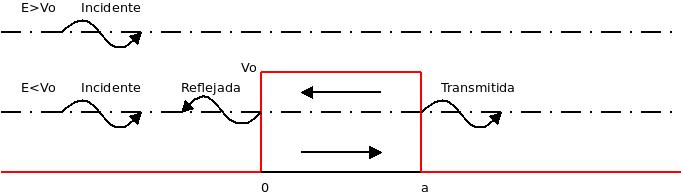
\includegraphics[scale=0.7]{Barrera.jpeg}
						\caption{Barrera de potencial}
					\end{center}
				\end{figure}		
							
				\begin{minipage}[t]{0.5\textwidth}	
				
				Si $E<V_0$:\\				
				
				\begin{center}
					$\displaystyle \psi(x)=Ae^{ik_1x}+Be^{-ik_1x} \text{ si } x<0 \text{ con } k_1=\frac{\sqrt{2mE}}{\hbar}$	
				\end{center}				
				\begin{center}
					$\displaystyle \psi(x)=Ce^{k_2x}+De^{-k_2x} \text{ si } 0<x<a \text{ , } k_2=\frac{\sqrt{2m(V_0-E)}}{\hbar}$	
				\end{center}			
				\begin{center}
					$\displaystyle \psi(x)=Fe^{ik_1x}+Ge^{-ik_1x} \text{ si } x>a \text{ con } k_1=\frac{\sqrt{2mE}}{\hbar}$	
				\end{center}			
				\begin{center}
					En $x>a$, no existe variación del potencial que produzca una reflexión: $G=0$
				\end{center}
				\begin{center}
					Aplicando	 las condiciones de contorno en $x=0$ y en $x=a$ para la función y su derivada es obtiene:
				\end{center}
				\begin{center}
					$\displaystyle A+B=C+D$	
				\end{center}		
				\begin{center}
					$\displaystyle A-B=-i\frac{k_2}{k_1}C+i\frac{k_2}{k_1}D$	
				\end{center}		
				\begin{center}
					$\displaystyle Ce^{(-ik_1+k_2)a}+De^{-(ik_1+k_2)a}=F$	
				\end{center}		
				\begin{center}
					$\displaystyle -i\frac{k_2}{k_1}Ce^{(-ik_1+k_2)a}+i\frac{k_2}{k_1}De^{-(ik_1+k_2)a}=F$	
				\end{center}							
				\begin{center}
					$\Downarrow$
				\end{center}
				\begin{center}
					$\displaystyle A=\frac{C}{2}\left(1-i\frac{k_2}{k_1}\right)+\frac{D}{2}\left(1+i\frac{k_2}{k_1}\right)$	
				\end{center}		
				\begin{center}
					$\displaystyle B=\frac{C}{2}\left(1+i\frac{k_2}{k_1}\right)+\frac{D}{2}\left(1-i\frac{k_2}{k_1}\right)$	
				\end{center}		
				\begin{center}
					$\displaystyle D=C\left[\frac{1+i\frac{k_2}{k_1}}{-1+i\frac{k_2}{k_1}}\right]e^{2k_2a}$	
				\end{center}						
								
				\begin{center}
					Coeficiente de Transmisión:\\
				\end{center}
				\begin{center}
					$\displaystyle T=\frac{v_1F^*F}{v_1A^*A}$
				\end{center}								
						
				\end{minipage}
				\begin{minipage}[t]{0.49\textwidth}	
				
				Si $E>V_0$:\\				
				
				\begin{center}
					$\displaystyle \psi(x)=Ae^{ik_1x}+Be^{-ik_1x} \text{ si } x<0 \text{ con } k_1=\frac{\sqrt{2mE}}{\hbar}$	
				\end{center}				
				\begin{center}
					$\displaystyle \psi(x)=Ce^{ik_2x}+De^{-ik_2x} \text{ si } 0<x<a \text{ , } k_2=\frac{\sqrt{2m(E-V_0)}}{\hbar}$	
				\end{center}			
				\begin{center}
					$\displaystyle \psi(x)=Fe^{ik_1x}+Ge^{-ik_1x} \text{ si } x>a \text{ con } k_1=\frac{\sqrt{2mE}}{\hbar}$	
				\end{center}			
				\begin{center}
					En $x>a$, no existe variación del potencial que produzca una reflexión: $G=0$
				\end{center}
				\begin{center}
					Aplicando	 las condiciones de contorno en $x=0$ y en $x=a$ para la función y su derivada es obtiene:
				\end{center}
				\begin{center}
					$\displaystyle A+B=C+D$	
				\end{center}		
				\begin{center}
					$\displaystyle A-B=\frac{k_2}{k_1}C-\frac{k_2}{k_1}D$	
				\end{center}		
				\begin{center}
					$\displaystyle Ce^{-i(k_1-k_2)a}+De^{-i(k_1+k_2)a}=F$	
				\end{center}		
				\begin{center}
					$\displaystyle \frac{k_2}{k_1}Ce^{-(ik_1-k_2)a}-\frac{k_2}{k_1}De^{-(ik_1+k_2)a}=F$	
				\end{center}		
				\begin{center}
					$\Downarrow$
				\end{center}
				\begin{center}
					$\displaystyle A=\frac{C}{2}\left(1+\frac{k_2}{k_1}\right)+\frac{D}{2}\left(1-\frac{k_2}{k_1}\right)$	
				\end{center}		
				\begin{center}
					$\displaystyle B=\frac{C}{2}\left(1-\frac{k_2}{k_1}\right)+\frac{D}{2}\left(1+\frac{k_2}{k_1}\right)$	
				\end{center}		
				\begin{center}
					$\displaystyle D=C\left[\frac{-k_1e^{ik_2a}+k_2e^{k_2a}}{k_2e^{-k_2a}+k_1e^{-ik_2a}}\right]$	
				\end{center}		
				
				\begin{center}
					Coeficiente de Transmisión:\\
				\end{center}
				\begin{center}
					$\displaystyle T=\frac{v_1F^*F}{v_1A^*A}$
				\end{center}			
				
			\end{minipage}
	
					\subsubsection{Efecto túnel}
					
						Una partícula de masa $m$ y energía total $E$ que incide sobre una barrera de potencial de altura $V_0>E$ y ancho finito $a$, tiene cierta probabilidad $T$ de penetrar la barrera y aparecer del otro lado. A este fenómeno se le llama \textbf{penetración de barrera }y se dice que \textit{la partícula hizo un túnel} a través de la misma. $T$ es extremadamente pequeña en el límite clásico.
					
				\subsection{Oscilador armónico}
					\subsubsection{Forma general}
					\subsubsection{Niveles de energía}
					\subsubsection{Interpretación}
		\section{Aplicaciones en tres dimensiones}
				\subsection{Pozo de potencial}
				\subsection{Separación de variables}
		\section{Análisis de potenciales seccionalmente constantes}		
				\subsection{Estados ligados}
				
					Si $\exists$ un potencial $V(\vect{r})$ y la energía determina una zona del espacio, restringiendo al movimiento, debido al valor de su energía, existen estados ligados, con un conjunto discreto de valores de energía desde el punto de vista cuántico.
					
				\subsection{Estados no ligados}			
		\section{Principios de la teoría formal de la Mecánica Cuántica}
				\subsection{Operadores-Autofunciones-Autovalores}
				
				\begin{table}[H]
					\begin{center}
						\begin{tabular}{c|c}
							$A$ (Variable) & $\hat{A}$ (Operador) \\ 
						\hline 
							$\hat{\vect{r}}$ & $\hat{\vect{r}}=(x,y,z)$ \\ 
						\hline 
							$\hat{\vect{p}}$ & $\frac{\hbar}{i} \vec{\nabla}_{\vect{r}} =\frac{\hbar}{i}(\frac{\partial}{\partial x},\frac{\partial}{\partial y},\frac{\partial}{\partial z})$ \\
						\hline 
							$\hat{\vect{L}}=\hat{\vect{r}} \times \hat{\vect{p}}$ & $\hat{\vect{L}}=\frac{\hbar}{i} \hat{\vect{r}} \times \vec{\nabla}_{\vect{r}}$ \\ 
						\hline 
							$V(\vect{r})$ & $V(\vect{r})$ \\ 
						\hline 
							$E$ & $\hat{\vect{H}}=-\frac{\hbar^2}{2m}\vec{\nabla}^2_{\vect{r}}+V(\vect{r})$ \\ 
						\end{tabular} 
						\caption{Operadores físicos}
					\end{center}
				\end{table}
				
				\subsection{Postulados}

					\begin{enumerate}
						\item \emph{El estado del sistema está representado por la función de onda $\Psi(\vect{r},t)$ en una determinada posición y tiempo}
						\item \emph{El resultado de una medición de una cantidad física $A$ tiene asociado un operador $\hat{A} \vert \hat{A}\Psi_a=a\Psi_a$}\\
						
						Siendo los autovalores $a$ el resultado de la medición y $\Psi_a$ la autofunción del operador $\hat{A}$
						
						Los autovalores pueden ser:\\
						
						\begin{itemize}
							\item Discretos (numerables): Asociados a los estados \emph{ligados}, definido por un potencial o restricciones\\
								\begin{itemize}
									\item No degenerados:$\{a_1,\ldots,a_n\},i=1,\ldots,n \in N, \exists! \text{ valor } a_i \text{ para cada } \Phi_i \vert \hat{A}\Phi_i=a_i\Phi_i$
									\item Degenerados:$\{a_{ij} \vert \hat{A}\Phi_j=a_{ij}\Phi_j \} \text{ No ligado a lo estocástico}$
								\end{itemize}
							
							\item Continuos: $\exists \text{ autovalores no numerables} \longrightarrow \hat{A}\Phi_a=a\Phi_a \text{ , } a \in \Re$  , asociado a estados \emph{no ligados}
						\end{itemize}
						
						\item \emph{La probabilidad de obtener en una medición un dado valor $a$, si la función de onda}
						
							\begin{center}
								$\Psi=\sum_j c_j \Phi_j \vert \hat{A}\Phi_j=a_j \Phi_j$ es $P(a_j)=\vert c_j \vert^2$
							\end{center}						
						
						\item \emph{La evolución temporal del sistema responde a la ecuación de Schrödinger:}
						
							\begin{center}
								$i \hbar \frac{\partial \Psi(\vect{r},t)}{\partial t}=\hat{H} \Psi(\vect{r},t)$	
							\end{center}
							
						\item \emph{El valor medio de la medición de una magnitud física $A$ se obtiene a partir de:}
						
							\begin{center}
								$\langle A \rangle=\int_{vol} \Psi^* (\vert{r},t)\left(\hat{A} \Psi(\vert{r},t)\right) dV$
							\end{center}													
					\end{enumerate}									
				
				\subsection{Valores medios de una magnitud física}
				\subsection{Superposición lineal de funciones de onda de estados estacionarios}
	
	\chapter{Átomo}
		\section{Átomo de Hidrógeno}	
		
			A diferencia de el espectro emitido por sólidos que han sido calentados, la radiación electromagnética de un átomo libre está concentrada en un número discreto de longitudes de onda. Cada átomo tiene su espectro característico.
			
			Para cada longitud de onda absorbida por un átomo, hay una correspondiente longitud de onda emitida. Sin embargo, la recíproca, no es cierta.

			Bohr desarrolló una teoría que predecía con gran precisión los espectros de algunos elementos, incluídos el de hidrógeno. La teoría era matemáticamente sencilla, pero recaía sobre cuatro postulados de dudosa aceptación:
			
			\begin{enumerate}
				\item Un electrón se mueve circularmente alrededor del núcleo atraído por fuerzas de Coulomb y bajo las reglas de la mecánica clásica.
				\item Sin embargo, en lugar de moverse en todas las órbitas posibles de le mecánica clásica, el electrón habita en órbitas para las cuales su momento cinético es $L=n \hbar$
				\item A pesar del hecho de que el electrón esté constantemente acelerando, el electrón se mueve de tal forma que no irradie energía. Por lo tanto, su energía total permanece constante.
				\item Radiación electromagnética es emitida únicamente cuando, un electrón moviéndose en una órbita de energía total $E_{i}$ cambia, discontinuamente, su movimiento para pasar a otra órbita de energía total $E_{j}$. La frecuencia de la radiación será: $\nu=(E_{i}-E_{j})/h$.
\end{enumerate}

				Como se puede observar, hay una gran mezcla entre la mecánica clásica y la cuántica. Por un lado los electrones se mueven circularmente clásicos, pero tienen niveles cuantizados de energía. El electrón es atraído por fuerzas de Coulomb, pero no emite radiación electromagnética a pesar de estar acelerado. También se asume que la masa del electrón es despreciable respecto de la del núcleo y que, por lo tanto, el núcleo está fijo. La energía total, por tanto será $E=E_c+E_V$ donde $E_c$ es la energía cinética y $E_V$ es la energía potencial eléctrica con referencia en el infinito.

				De acuerdo a Bohr, para átomos de un sólo electrón, las posibles órbitas son aquellas de radio $r$ y velocidad $v$ 

				\begin{center}
					$r=\frac{\hbar^{2}4\pi \epsilon_{0}}{m_{0}e^{2}Z} n^{2} \qquad ; \qquad v=\frac{e^{2}}{4 \pi \epsilon_{0} \hbar} \cdot \frac{1}{n}$
				\end{center}

				Para $n=1$ la velocidad es del orden del $1\%$ de la velocidad de la luz y, por lo tanto, se justifica el postulado sobre mecánica clásica de Bohr. Para átomos con gran número atómico ($Z$) la velocidad se acerca a la de la luz y la teoría de Bohr no aplica.

La energía total de cada órbita es 

				\begin{center}
					$E=\frac{m_0}{2} \left( \frac{e^2 Z}{4 \pi \epsilon_0 \hbar^2} \right)^2 \cdot \frac{1}{n^{2}}$
				\end{center}

				La cuantización del momento cinético lleva a la cuantización de la energía. La energía es negativa porque el cero del potencial electrostático se define en el punto en que el electrón está suelto del átomo.

				La frecuencia de las radiaciones electromagnéticas será 

				\begin{center}
					$\nu=\frac{m_0}{2} \frac{e^4 Z^2}{8 \pi^2 \epsilon_0 \hbar^3} \left( \frac{1}{n_f^2}-\frac{1}{n_i^2} \right)$
				\end{center}

				o, según el número de onda, $k=R_{y}(1/n_{f}^{2}-1/n_{i}^{2})$ con $R_{y}=10^{6}\textrm{m}^{-1}$.		
		
			\subsection{Ecuación de Schrödinger en coordenadas esféricas}
				\subsubsection{Cuantización del momento angular}
				
					Sabemos que el operador asociado al momento angular es $\hat{L}=\vect{r} \times \hat{p}$, con $\vert \vect{L} \vert^2=cte$ independiente del tiempo, impuesto por Bohr, aunque contradice a Maxwell.
					
					¿Cuáles son los autovalores del operador? Se debe realizar una transformación a coordenadas esféricas:
					
					\begin{center}
						$\vect{r} \longrightarrow (\theta,\phi,r)=\begin{Bmatrix}{x=r \sin \theta \cos \phi} \\ y=r \sin \theta \sin \phi \\ z=r \cos \theta \end{Bmatrix}=\begin{Bmatrix}{r=\sqrt{x^2+y^2+z^2}} \\ \theta=\sin^{-1} \left( \frac{\sqrt{x^2+y^2}}{r} \right) \\ \phi=\tan^{-1} \left( y/x \right) \end{Bmatrix}$\\
						
						$\vec{\nabla}^2_{(r,\phi,\theta)}=\frac{1}{\sin \theta}\frac{\partial}{\partial \theta} \left( \sin \theta \frac{\partial}{\partial \theta} \right)+\frac{1}{\sin^2 \theta}\frac{\partial^2}{\partial \phi^2}$\\
						
						$\hat{\vect{L}}^2 Y(\theta,\phi)=-\hbar^2 \nabla^2 Y_{m,l}(\theta,\phi)=\underbrace{-\hbar^2 l(l+1)}_{\text{Autovalor}}\underbrace{Y_{m,l}(\theta,\phi)}_{\text{Autofunción}} \text{ , } l=0,1,2,\ldots$
					\end{center}
				
					Las autofunciones de $\hat{\vect{L}}^2$ son los armónicos esféricos $Y_{m,l}(\theta,\phi)$ con \textbf{m:número cuántico magnético} y \textbf{l:número cuántico orbital}. Los autovalores de $\hat{\vect{L}}^2$ son $-\hbar^2 l(l+1) \text{ , } l=0,1,2,\ldots$. Se encuentra que $\vert m \vert \leq l \longrightarrow -l \leq m\leq l$
								
					\begin{center}
						$\begin{Bmatrix}{\frac{\partial}{\partial x}=\frac{\partial r}{\partial x}\frac{\partial}{\partial r}+\frac{\partial \theta}{\partial x}\frac{\partial}{\partial \theta}+\frac{\partial \phi}{\partial x}\frac{\partial}{\partial \phi}} \\ \frac{\partial}{\partial y}=\frac{\partial r}{\partial y}\frac{\partial}{\partial r}+\frac{\partial \theta}{\partial y}\frac{\partial}{\partial \theta}+\frac{\partial \phi}{\partial y}\frac{\partial}{\partial \phi} \\ \frac{\partial}{\partial z}=\frac{\partial r}{\partial z}\frac{\partial}{\partial r}+\frac{\partial \theta}{\partial z}\frac{\partial}{\partial \theta}+\frac{\partial \phi}{\partial z}\frac{\partial}{\partial \phi} \end{Bmatrix}  \Rightarrow \begin{Bmatrix}{\hat{L}_x=i\hbar \left(\sin \phi \frac{\partial}{\partial \theta}+\cot \theta \cos \phi \frac{\partial}{\partial \phi}\right)} \\ \hat{L}_y=i\hbar \left(-\cos \phi \frac{\partial}{\partial \theta}+\cot \theta \sin \phi \frac{\partial}{\partial \phi}\right) \\ \hat{L}_z=-i\hbar \frac{\partial}{\partial \phi} \end{Bmatrix}$
					\end{center}					
					
				\subsubsection{Funciones de onda radiales y angulares}		
					
					Si considero que las variables son separables $Y_{m,l}(\theta,\phi)=\Theta_{m,l}(\theta)\Phi_m(\phi)$					
					
					 y me enfoco solamente en la coordenada $z$:\\
					
					\begin{center}
						$\hat{L}_z \Phi(\phi)=-i \cancel{\hbar} \frac{\partial \Phi_m(\phi)}{\partial \phi}=m \Phi_m(\phi)\cancel{\hbar} \Rightarrow$ \boxed{\Phi_m(\phi)=\phi_0 e^{\pm i m \phi}} $\text{ , } m=0,\pm 1,\pm 2,\ldots$\\
						
						$\hat{\vect{L}} \cdot \hat{\vect{L}}=\hat{\vect{L}}^2=\hat{L}_x^2+\hat{L}_y^2+\hat{L}_z^2=-\hbar^2 \vec{\nabla}_{\Theta,\Phi}^2$
						
						$\hat{\vect{L}}^2=-\hbar^2 \left[\frac{1}{\sin \theta}\frac{\partial}{\partial \theta}\left(\sin \theta \frac{\partial}{\partial \theta} \right)+\frac{1}{\sin^2 \theta}\frac{\partial^2}{\partial \phi^2}\right]$
					\end{center}
					
					Luego con $\Theta_{m,l} (\theta)=P_l^m \underbrace{\left( \cos \theta \right)}_X$. Sea un polinomio de legendre que cumpla\\
					 
					\begin{center}
						$\frac{(1-x^2)^{m/2}}{2l!}\frac{d^{l+m}}{d x^{l+m}}(x^2-1)^l \Rightarrow Y_{m,l}(\theta,\phi)=\phi_0 e^{i m \phi}P_l^m(\cos \theta)$
					\end{center}				
					
				\subsubsection{Densidad de probabilidad radial}
					
					Para el átomo de Hidrógeno se cumple $\hat{\vect{H}} \underbrace{\Psi_T (\vect{r}_e,\vect{r}_p)}_{\text{electrón-protón}}=\epsilon \Psi_T (\vect{r}_e,\vect{r}_p)$ con el operador Hamiltoniano $\hat{\vect{H}}=\frac{-\hbar^2}{2 m_p}\vec{\nabla}_{r_p}^2+\frac{-\hbar^2}{2 m_e}\vec{\nabla}_{r_e}^2+V(\vert \vect{r}_e-\vect{r}_p \vert)$. El problema se aborda con un cambio de coordenadas:\\
					
					\begin{center}
						$\vect{R}=\frac{\vect{r}_e m_e+\vect{r}_p m_p}{m_e+m_p} \qquad \vect{r}=\vect{r}_e-\vect{r}_p \qquad M=m_e+m_p \qquad \mu=\frac{m_e m_p}{m_e+m_p}$\\
						
						$\Downarrow$\\
						
						$\Psi_T(\vect{r},\vect{R})=\Psi(\vect{r}) S(\vect{R}) \qquad \hat{\vect{H}}=\frac{-\hbar^2}{2M}\vec{\nabla}_{\vect{R}}+\frac{-\hbar^2}{2 \mu}\vec{\nabla}_{\vect{r}}+V(\vect{r})$\\
						
						$\Downarrow$\\
						
						$\frac{-\hbar^2}{2M}\Psi(\vect{r})\vec{\nabla}_R^2 S(\vect{R})+\frac{-\hbar^2}{2\mu}S(\vect{R})\vec{\nabla}_r^2\Psi(\vect{r})+V(\vect{r})\Psi(\vect{r}) S(\vect{R})=\epsilon\Psi(\vect{r}) S(\vect{R})$\\
						
						$\Downarrow$\\
						
						$\frac{-\hbar^2}{2M}\frac{\vec{\nabla}_R^2S(\vect{R})}{S(\vect{R})}=\epsilon+\frac{-\hbar^2}{2\mu}\frac{\vec{\nabla}_r^2\Psi(\vect{r})}{\Psi(\vect{r})}-V(\vect{r})=\epsilon_{\text{Centro de masa}}$\\
						
						$\Downarrow$\\
						
						$\frac{-\hbar^2}{2M}\vec{\nabla}_R^2S(\vect{R})=\epsilon_{\text{Centro de masa}} S(\vect{R}) \Rightarrow$ \boxed{S(\vect{R})=cte \cdot e^{i \vect{K} \cdot \vect{R}}}
					\end{center}
					
					Falta resolver la ecuación diferencial para el electrón en el átomo de Hidrógeno, considerando $\mu \simeq m_e$ y utilizando el laplaciano en esféricas\\
					
					\begin{center}
						$\frac{-\hbar^2}{2\mu}\vec{\nabla}_r^2\Phi(\vect{r})+V(\vect{r})\Phi(\vect{r})=\epsilon \Phi(\vect{r})$\\
						
						$\Downarrow$\\
						
						$\frac{-\hbar^2}{2\mu r^2}\left[\frac{\partial}{\partial r}\left( r^2 \frac{\partial}{\partial r}\Psi(\vect{r})\right)+\frac{1}{\sin \theta}\frac{\partial}{\partial \theta}\left( \sin \theta \frac{\partial \Psi(\vect{r})}{\partial \theta}\right)+\frac{1}{\sin^2 \theta}\frac{\partial^2}{\partial \phi^2}\Psi(\vect{r}) \right]+V(\vect{r})\Psi(\vect{r})=\epsilon \Psi(\vect{r})$\\
						
						$\Downarrow$\\
						
						$\frac{-\hbar^2}{2\mu r^2}\frac{\partial}{\partial r}\left( r^2 \frac{\partial}{\partial r}\Psi(\vect{r})\right)+\frac{\hat{\vect{L}}^2}{2\mu r^2}\Psi(\vect{r})+V(\vect{r})\Psi(\vect{r})=\epsilon \Psi(\vect{r})$\\
								
						$\Downarrow$\\				
					
						Propongo $\Psi(\vect{r})=R(\vect{r})Y_{m,l}(\theta,\phi)$\\
						
						$\Downarrow$\\
						
						$\frac{1}{r^2}\frac{d}{dr}\left(r^2 \frac{d}{dr}R(\vect{r})\right)+\frac{2\mu r^2}{\hbar^2}\left(\epsilon+\underbrace{\frac{e^2}{4\pi \epsilon_0 r}}_{\begin{subarray}{l}\text{Potencial}\\ \text{Coulombiano}\end{subarray}}-\overbrace{\frac{l(l+1)}{r^2}}^{\begin{subarray}{l}\text{Aceleración}\\ \text{Centripeta}\end{subarray}}\right)R(\vect{r})=0$\\
						
						$\Downarrow$\\
						
						Considerando $R(\vect{r})=\frac{X(\vect{r})}{r} \qquad K=\frac{1}{4\pi \epsilon_0}$\\
						
						$\Downarrow$\\
						
						$\frac{d^2 X(\vect{r})}{d r^2}+\frac{2\mu r^2}{\hbar^2}\left[ \epsilon+\frac{e^2}{Kr}-\frac{l(l+1)}{r^2}\right] X(\vect{r})=0$
						
						$\Downarrow$\\
						
						Porque: $\lim_{r \to 0}R(\vect{r})=0 \quad \lim_{r \to 0}V(\vect{r})=\infty \quad \lim_{r \to \infty}R(\vect{r})=0 \quad \lim_{r \to \infty}B(\vect{r})=0 \Rightarrow R(\vect{r}) \sim 1/r$\\
						
						$\Downarrow$\\
						
						Aproximando a $X(\vect{r})$ por un polinomio de Laguerre, aparece como condición de la convergencia de la solución un número natural \textbf{$n=1,2,3,\ldots$ número cuántico principal} que cumple $l \leq n-1$
						
						$\Downarrow$\\
						
						$R_{n,l}(\vect{r})=A_{n,l} e^{-\frac{r}{n a_0}}\left(\frac{2r}{n a_0}\right)^l L_{n,l} \left(\frac{2r}{n a_0}\right)$
					\end{center}
					
					La solución general de la función de onda del electrón en el átomo de Hidrógeno:\boxed{\Psi_{n,l,m}(\vect{r},\phi,\theta)=R_{n,l}(\vect{r}) Y_{l,m}(\theta,\phi)}

			\subsection{Spin del electrón}				
				\subsubsection{Experimento de Stern-Gerlach}
					
					Stern-Gerlach estudiaban el momento magnético de átomos a muy baja energía. Utilizando un horno a aproximadamente $1000^o C$ con átomos de plata y una rendija. A la salida ponen 2 polos de electroimanes para concentrar las líneas de campo magnético $\vect{H}$.\\
					
					En la experiencia se esperaba que en la rendija se genere un patrón lineal continuo. En cambio lo que se manifestó fueron dos sitios puntuales muy marcados. Dirac interpretó que faltaba definir un cuarto número cuántico para completar la teoría.\\
					
					Existe un impulso angular intrínseco denominado spin: $\hat{\vect{S}}^2 \chi=\hbar(s^2+s)\chi \longrightarrow \vert \vect{S} \vert=\frac{\hbar}{2}$.\\
					
					Considerando $+\hbar/2$: \textit{Spin Up} y $-\hbar/2$: \textit{Spin Down}
					
					Añadiendo complejidad a la ecuación de onda: \boxed{\Psi_{n,l,m,s}(\vect{r},\theta,\phi)=R_{n,l}(\vect{r}) Y_{l,m}(\theta,\phi)\chi_s}
					
				\subsubsection{Densidad de probabilidad del electrón en el átomo de Hidrógeno}
					
					$P(\vect{r})=\int_0^{2\pi}\int_0^{\pi}\int_0^{r} \Psi^*_{n,l,m,s}(\vect{r},\theta,\phi)\Psi_{n,l,m,s}(\vect{r},\theta,\phi) \underbrace{r^2 dr d\phi \sin \theta d\theta}_{d\Omega}$
					
					La densidad de probabilidad angular será una constante, por lo que será mas conveniento resolver únicamente la densidad de probabilidad radial $P(r)=cte\int_0^r r^2 R_{n,l}^2(r) dr$ de encontrar al electrón a una distancia del protón.
					
				\subsubsection{Similitudes con Bohr}				
					
					Por ejemplo para algunos valores de n y l:				
					
					\begin{center}
						$R_{1,0}(r)=2 e^{-r/a_0}$\\
						
						$R_{2,0}(r)=\frac{\sqrt{2}}{4}\left(2-\frac{r}{a_0}\right) e^{-\frac{r}{2a_0}}$\\
						
						$R_{2,1}(r)=\frac{\sqrt{6}}{12}\left(\frac{r}{a_0}\right)e^{-\frac{-r}{2a_0}}$\\
						
						$R_{3,0}(r)=\frac{2\sqrt{3}}{27}\left(1-\frac{2r}{a_0}+\frac{2}{9}\left(\frac{r}{a_0}\right)^2\right)e^{-\frac{r}{3a_0}}$\\
					\end{center}
					
					Los mñaximos de $P(r)$ coinciden con los radios de las \textbf{órbitas de Bohr}: $r_n=a_0 n^2$
		
		\section{Átomos multielectrónicos}
		
			\begin{itemize}
				\item La energía está cuantizada: $E_n=\frac{-E_0}{n^2} \text{ , } n=1,2,3,\ldots \text{ , } E_0=13.6 eV$ energía de ionización.
				\item Las funciones de onda, orbitales, y su $\Psi^2$ representa la densidad de probabilidad y dependen de las coordenadas esféricas $(r,\theta,\phi)$. No existe ninguna órbita, solo existen nubes de probabilidad.
				\item Existen cuatro números para definir cada órbita: $n=1,2,3,\ldots$, $l \leq n-1$, $-l \leq m \leq l$, $s=\pm 1/2$
			\subsection{Principio de exclusión de Pauli}	
				\item En átomos de mas electrones, se cumple el \emph{principio de exclusión de Pauli}. No existen dos electrones con los mismos números cuánticos. Si n,m y l son iguales entre dos electrónes, entonces diferirán en el spin.
				\item El impulso angular está cuantizado
				\item El spin también está cuantizado
			\subsection{Estructuras de las capas electrónicas de los átomos}
				\item La forma de construir átomos multielectrónicamente es llenando los orbitales mediante la \textbf{regla de Hund}. Obteniendo la \textbf{configuración electrónica} del átomo
			\end{itemize}					
								
	\chapter{Física estadística}
		\section{Conceptos generales}
		
			El objetivo es el analizar el comportamiento de un gran conjunto de partículas o sistemas idénticos, en una forma estadística o probabilística, derivando los valores más probables de las propiedades del conjunto sin abordar en detalle los valores de estas propiedades para una partícula dada en un momento determinado.\\
			
			El sistema de partículas posee una energía interna total $U$, una cantidad de partículas $N$ y una función de onda $\Psi (\vec{r},t)$ que lo describe. La distribución de energía en las cuales se ubican las partículas depende de la densidad de estados de energía y de la probabilidad de que un estado sea ocupado, dada por la función de onda.
			
			\begin{center}
				$\displaystyle n(\varepsilon) \delta\varepsilon=g(\varepsilon)f(\varepsilon)\delta\varepsilon$
			\end{center}

			\begin{itemize}
				\item $n(\varepsilon)$: Cantidad de partículas por unidad de volumen con energías comprendidas entre $\varepsilon$ y $\varepsilon+\delta\varepsilon$.
				\item $\delta\varepsilon$: Intervalo de energía.
				\item $g(\varepsilon)$: Densidad de estados o número de estados de energía por unidad de volumen con energías comprendidas entre  $\varepsilon$ y $\varepsilon+\delta\varepsilon$.Siempre es función de la energía.
				\item $f(\varepsilon)$: Función de distribución o probabilidad de que esté en el estado de energía $\varepsilon$.\\
			\end{itemize}					
			
			Las limitaciones físicas sobre las partículas determinan la forma de $g(\varepsilon)$. Por ejemplo, si se trata de electrones en metales $\displaystyle g(\varepsilon)=\frac{4\pi (2m)^{3/2}}{h^3}\sqrt{\varepsilon}$ y para fotones donde se cumple la relación de De Broglie ($\varepsilon=h c/\lambda$) se tiene $\displaystyle g(\varepsilon)=\frac{8\pi}{(hc)^3}\varepsilon^2$\\
			
			\begin{itemize}
				\item Maxwell-Boltzmann: $\displaystyle F(\varepsilon)=\frac{1}{A e^{\frac{\varepsilon}{kT}}}$, clásica. Se aplica para partículas idénticas y distinguibles, gas ideal clásico.
				\item Fermi-Dirac: $\displaystyle F(\varepsilon)=\frac{1}{A e^{\frac{\varepsilon}{kT}}+1}$, cuántica. Se aplica para partículas idénticas e indistinguibles que cumplen el principio de exclusión de Pauli (Fermiones), spin semientero, su función de onda es antisimétrica. Gas de electrones en metales.
				\item Bose-Einstein: $\displaystyle F(\varepsilon)=\frac{1}{A e^{\frac{\varepsilon}{kT}}-1}$, cuántica. Se aplica para partículas idénticas e indistinguibles que no cumplen el principio de exclusión de Pauli (Bosones), spin entero, su función de onda es simétrica. Radiación térmica, calor específico, fotones, fonones.
			\end{itemize}
			
			Donde $A$ es una constante de normalización tal que $\displaystyle \int_0^\infty f(\varepsilon)d\varepsilon=1$\\
								
			\subsection{Macro estados y Micro estados}
		
				Un \textbf{microestado} es la especificación detallada de una configuración microscópica de un sistema termodinámico. En otros términos, un microestado es un punto del espacio fásico de dicho sistema.\\
				
				Un \textbf{macroestado} se refiere a una caracterización del sistema termodinámico mediante los valores de un número finito n de variables de estado, de las cuales al menos una de ellas es una magnitud extensiva. El macroestado obedece por tanto a una descripción macroscópica. Un macroestado viene dado por una distribución de probabilidad sobre un conjunto dado de microestados; en función del conjunto de microestados considerado, la distribución toma una forma u otra. Un sistema en equilibrio permanece en un macroestado (macroestado de equilibrio) mientras visita los diferentes microestados accesibles a lo largo de sus fluctuaciones			
			
			\subsection{Equilibrio térmico o estadístico}
			
			Un sistema en equilibrio no tiene ninguna preferencia por ninguno de los microestados disponibles para ese equilibrio. Si $ \Omega$ es el número de microestados disponibles para una cierta energía, entonces la probabilidad de encontrar el sistema en uno cualquiera de esos microestados es $p=\frac{1}{\Omega}$. Dado un sistema en equilibrio, el estado termodinámico (macroestado) que está asociado a un mayor número de microestados es el macroestado más probable del sistema.\\
			
			\subsection{Partículas distinguibles e indistinguibles}
				
				Se define un conjunto de partículas \textbf{idénticas} como aquellas que comparten la misma naturaleza física.\\
				
				Las partículas se consideran que son \textbf{indistinguibles}, si sus paquetes de ondas se solapan significativamente. Este tipo de consideración viene del hecho, de que de acuerdo con la hipótesis de De Broglie, todas las partículas tienen propiedades características de onda. Dos partículas se pueden considerar \textbf{distinguibles}, cuando sus funciones de onda no se solapan, es decir si su separación es grande en comparación con su longitud de onda de De Broglie.\\	
			
		\section{Estadística Clásica}
		
			Aplicable para un conjunto de partículas idénticas y distinguibles (Gases ideales por ejemplo), donde no existan restricciones a los valores de energía y cantidad de movimiento para las partículas del sistema. Los sucesos son equiprobables
			
			\subsection{Ley de distribución de Maxwell-Boltzmann}

				\begin{center}
					\boxed{\displaystyle f(\varepsilon)=A e^{-\frac{\varepsilon}{kT}}=\frac{n(\varepsilon)}{g(\varepsilon)}}
				\end{center}
				
				Donde $A$ es una constante de normalización tal que $\displaystyle \int_0^\infty f(\varepsilon)d\varepsilon=1$
				
			\subsection{Función de partición del sistema}
			
				La función de partición o suma sobre estados es una fórmula matemática que expresa una suma de factores de probabilidad de los diferentes microestados. Los términos de esta suma regulan el modo como se distribuyen las partículas del colectivo en los diferentes microestados. La función de partición es la herramienta matemática principal de la termodinámica estadística. A partir de ella se obtiene toda la información termodinámica sobre el sistema, por lo cual se dice que la función de partición representa en termodinámica estadística un papel análogo al que representa la función de onda en la teoría cuántica.\\
				
				Se define  $\displaystyle Z=\sum_i g_i(\varepsilon) e^{-\frac{\varepsilon_i}{kT}}$ en el caso discreto y $\displaystyle Z=\int_\varepsilon g(\varepsilon) e^{-\frac{\varepsilon}{kT}}d\varepsilon$ en el caso continuo.
			
			\subsection{Energía promedio del sistema}
	
				$\displaystyle \langle\varepsilon\rangle$	: Valor medio de energía por partícula.\\
				
				Partiendo de un estado de equilibrio termodinámico y equiprobable para todas las partículas, consistente con $N$ y $U$				
				
				Considerando que en este caso $g(\varepsilon)=g=1$. Normalizando: $\displaystyle f(\varepsilon)=\frac{e^{-\frac{\varepsilon}{kT}}}{kT}$\\
				
				\begin{center}
					\boxed{\displaystyle \langle\varepsilon\rangle=\int_0^\infty \varepsilon \frac{e^{-\frac{\varepsilon}{kT}}}{kT}=kT}
				\end{center}
			
			\subsection{Distribución de energías,momentos y velocidades}
			
				\begin{itemize}
					\item Distribución de energía: \boxed{\displaystyle F(\varepsilon)=\frac{e^{-\frac{\varepsilon}{kT}}}{kT}}
								
					\item Distribución de momentos: Analizando en una dimensión: $E_c=\frac{p_z^2}{2m}$ entonces $\displaystyle F(p_z)=A e^{-\frac{ p_z^2}{2mkT}}$. Al normalizar se encuentra \boxed{\displaystyle F(p_z)=\sqrt{\frac{2}{m\pi kT}}e^{-\frac{p_z^2}{2mkT}}}.
					
					\item Distribución de velocidades: Analizando en una dimensión: $E_c=\frac{1}{2}m v_z^2$ entonces $\displaystyle F(v_z)=A e^{-\frac{m v_z^2}{2kT}}$. Al normalizar se encuentra \boxed{\displaystyle F(v_z)=\sqrt{\frac{2m}{\pi kT}} e^{-\frac{m v_z^2}{2kT}}}.
				\end{itemize}
			
			\subsection{Velocidad media cuadrática y mas probable}
			
				\begin{itemize}
					\item Velocidad media cuadrática: $\displaystyle \langle v_z^2 \rangle=\int_{-\infty}^{\infty} v_z^2 \sqrt{\frac{2m}{\pi kT}} e^{-\frac{m v_z^2}{2kT}} dv_z=\frac{kT}{m} \longrightarrow $ \boxed{\displaystyle \langle \vec{v}^2 \rangle=3\frac{kT}{m}}
					
					\item Velocidad media cuadrática: $\displaystyle \langle v_z \rangle=\int_{-\infty}^{\infty} v_z \sqrt{\frac{2m}{\pi kT}} e^{-\frac{m v_z^2}{2kT}} dv_z=\sqrt{\frac{2 kT}{\pi m}} \longrightarrow $ \boxed{\displaystyle \langle \vec{v}\rangle=\sqrt{\frac{8 kT}{\pi m}}}
				\end{itemize}
			
			\subsection{Energía total de las moléculas de un gas}	
			
				En un gas ideal, la densidad de estados será $\displaystyle g(\varepsilon)=\frac{4(2m^3)^{1/2}\pi V}{h^3}\sqrt{\varepsilon}$ y $\displaystyle Z=\int_0^\infty g(\varepsilon) e^{-\frac{\varepsilon}{kT}}d\varepsilon$\\
				
				\begin{center}
					$\displaystyle U=\int_0^\infty \varepsilon N(\varepsilon)d\varepsilon=\int_0^\infty \varepsilon f(\varepsilon)g(\varepsilon)d\varepsilon=\int_0^\infty \varepsilon e^{-\frac{\varepsilon}{kT}}\frac{N}{Z}\frac{4(2m^3)^{1/2}\pi V}{h^3}\sqrt{\varepsilon}d\varepsilon$\\
				\end{center}
				\begin{center}	
					$\displaystyle U=\frac{4(2m^3)^{1/2}\pi V}{h^3}\frac{N}{\int_0^\infty g(\varepsilon) e^{-\frac{\varepsilon}{kT}}d\varepsilon}\int_0^\infty \varepsilon^{3/2} e^{-\frac{\varepsilon}{kT}} d\varepsilon=\frac{4(2m^3)^{1/2}\pi V}{h^3} \frac{N}{\int_0^\infty g(\varepsilon) e^{-\frac{\varepsilon}{kT}}d\varepsilon} \frac{3 \sqrt{\pi} (kT)^{5/2}}{4}$
				\end{center}
				\begin{center}
					$\displaystyle U=\frac{N}{ \int_0^\infty \sqrt{\varepsilon}e^{-\frac{\varepsilon}{kT}}d\varepsilon} \frac{3 \sqrt{\pi} (kT)^{5/2}}{4}=\frac{N}{\frac{\sqrt{\pi}(kT)^{3/2}}{2}} \frac{3 \sqrt{\pi} (kT)^{5/2}}{4}$
				\end{center}
				\begin{center}
					\boxed{\displaystyle U=\frac{3}{2}NkT} $\longrightarrow$ \boxed{\displaystyle C_v=\left(\frac{\partial U}{\partial T}\right)_v=\frac{3}{2}Nk}
				\end{center}
			
		\section{Conceptos de Estadísticas Cuánticas}	
		
					La estadística cuántica nace como extensión de la estadísitica clásica, debido a las limitaciones propias de la naturaleza que me imide aplicar la teoría clásica ($\Delta p \Delta x \sim \hbar/2$ por Heisemberg). Se trabaja en 6 dimensiones (sextupla) de posicones y momentos.\\
			
				\subsection{Indistinguibilidad de partículas idénticas}
				
					Se llaman idénticas a las partículas con la misma estructura y propiedades (spin,carga,masa, etc). Cada partícula tiene asociada una función de onda que la caracteriza. Si la distancia que separa a ambas partículas es menor que las longitudes de ondas de De Broglie de las mismas, entonces las funciones de onda se solapan y estamos frente a partículas indistinguibles.\\
				
				\subsection{Funciones de onda simétrica y antisimétrica}

					Si considero un sistema de dos partículas relacionadas por una función de onda del sistema de la forma $\displaystyle \Psi(\vec{r}_1,\vec{r}_2)$.  Puedo asumir que al intercambiar el orden de las partículas tengo una función de onda proporcional a la anterior  $\displaystyle \Psi(\vec{r}_1,\vec{r}_2)=\gamma \Psi(\vec{r}_2,\vec{r}_1)$. Entonces si $\displaystyle \Psi(\vec{r}_1,\vec{r}_2)=C_{12}\Psi_a(\vec{r}_1)\Psi_b(\vec{r}_2)+C_{21}\Psi_a(\vec{r}_2)\Psi_b(\vec{r}_1)$:\\
					
					\begin{center}
						$\displaystyle \Psi(\vec{r}_1,\vec{r}_2)=\gamma\Psi(\vec{r}_2,\vec{r}_1)=\gamma(C_{12}\Psi_a(\vec{r}_2)\Psi_b(\vec{r}_1)+C_{21}\Psi_a(\vec{r}_1)\Psi_b(\vec{r}_2)) \underbrace{\Rightarrow}_{\gamma= \pm 1}$\\
						$\displaystyle \Psi_a(\vec{r}_1)\Psi_b(\vec{r}_2)(C_{12} \pm C_{21})=\Psi_a(\vec{r}_2)\Psi_b(\vec{r}_1)(C_{12} \mp C_{21})$ 
					\end{center}
				
					La igualdad se cumple si $C_{12}=\pm C_{21}$ y la función de onda del sistema será:\\
					
					\begin{center}
						$\displaystyle  \Psi(\vec{r}_1,\vec{r}_2)=C\left[\Psi_a(\vec{r}_1)\Psi_b(\vec{r}_2) \pm \Psi_a(\vec{r}_2)\Psi_b(\vec{r}_1)\right]$
					\end{center}			
				
				\subsection{Bosones y Fermiones}
				
					\begin{itemize}
						\item Bosones
							\begin{itemize}
								\item Función de onda simétrica $\displaystyle  \Psi(\vec{r}_1,\vec{r}_2)=C\left[\Psi_a(\vec{r}_1)\Psi_b(\vec{r}_2) + \Psi_a(\vec{r}_2)\Psi_b(\vec{r}_1)\right]$
								\item Spin entero $\displaystyle \vert \vec{s} \vert=0,\hbar,2\hbar,\ldots $(Spin nulo para los fotones)
								\item NO cumplen el principio de exclusión de Pauli
								\item Estadística de Bose-Einstein
								\item Fotones(cuantos de radiación electromagnética), Fonones(cuantos de vibración mecánica de iones),etc.
							\end{itemize}
						\item Fermiones
							\begin{itemize}
								\item Función de onda antisimétrica $\displaystyle  \Psi(\vec{r}_1,\vec{r}_2)=C\left[\Psi_a(\vec{r}_1)\Psi_b(\vec{r}_2) - \Psi_a(\vec{r}_2)\Psi_b(\vec{r}_1)\right]$
								\item Spin semientero $\displaystyle \vert \vec{s} \vert=\frac{1}{2}\hbar,\frac{3}{2}\hbar,\ldots $
								\item Cumple con el principio de exclusión de Pauli
								\item Estadística de Fermi-Dirac
								\item Electrones, protones, neutrones
							\end{itemize}
					\end{itemize}									
				
		\section{Estadística de Fermi-Dirac}
		
			La estadística de Fermi-Dirac es la forma de contar estados de ocupación de forma estadística en un sistema de fermione, tiene aplicaciones sobre todo en la Física del estado sólido.\\
			
			La energía de un sistema mecanico-cuántico está discretizada. Esto quiere decir que las partículas no pueden tener cualquier energía, sino que ha de ser elegida de entre un conjunto de valores discretos. Para muchas aplicaciones de la física es importante saber cuántas partículas están a un nivel dado de energía. La distribución de Fermi-Dirac nos dice cuánto vale esta cantidad en función de la temperatura y el potencial.\\
			
			\subsection{Densidad de estados g(E)}
			
				\begin{center}
					\boxed{\displaystyle g(\varepsilon)=\frac{g_s 4\pi V (2m^3)^{1/2}}{h^3}\varepsilon^{1/2}}
				\end{center}			
			
			\subsection{Ley de distribución de Fermi-Dirac}
			
				\begin{center}
					\boxed{\displaystyle F(\varepsilon)=\frac{1}{e^{\frac{\varepsilon-\varepsilon_f}{kT}}+1}}
				\end{center}
			
			\subsection{Nivel de Fermi}
			
				Para bajas temperaturas, la distribución de fermi es una función escalón que vale 1 si $\varepsilon<\varepsilon_f$ y 0 si $\varepsilon>\varepsilon_f$. Esto quiere decir que las partículas van colocando desde el nivel más bajo de energía hacia arriba debido al Principio de exclusión de Pauli hasta que se hayan puesto todas las partículas. La energía del último nivel ocupado se denomina energía de Fermi y la temperatura a la que corresponde esta energía mediante $\varepsilon_f=k T_f$, siendo $T_f$ la temperatura de Fermi.\\		
				
				$\displaystyle n=\frac{N}{V}=\int_0^\infty \frac{1}{V}\left(\frac{dn}{d\varepsilon}\right)_{FD} d\varepsilon=\int_0^\infty \frac{1}{V} g(\varepsilon)f_{FD}(\varepsilon) d\varepsilon \underbrace{\Longrightarrow}_{\text{si } T\simeq 0 K} n \simeq \int_0^{\varepsilon_f} \frac{1}{V} \frac{4\pi g_s V (2m^3)^{1/2}}{h^3} \varepsilon^{1/2} \underbrace{f_{FD}(\varepsilon)}_{1} d\varepsilon$
				
				\begin{center}
					$\displaystyle  n \simeq \int_0^{\varepsilon_f} \frac{4\pi g_s (2m^3)^{1/2}}{h^3} \varepsilon^{1/2}  d\varepsilon=\frac{4\pi g_s (2m^3)^{1/2}}{h^3} \int_0^{\varepsilon_f} \varepsilon^{1/2}  d\varepsilon=\frac{4\pi g_s (2m^3)^{1/2}}{h^3} \frac{2}{3}\varepsilon_f^{3/2}$
				\end{center}
				
				\begin{center}
					\boxed{\displaystyle \varepsilon_f \simeq \left[\frac{3 n h^3}{8\pi g_s (2m^3)^{1/2}}\right]^{2/3}} $\longrightarrow$ \boxed{\varepsilon_f \simeq cte \cdot n^{2/3}}
				\end{center}
			
			\subsection{Gas de electrones}
			
				Se tiene un gas de electrones, con un número grande de partículas fermiónicas con sus números de estados discretizados a temperatura $T= 0K$ o temperaturas bajas $T \sim T_0$.\\
				
				Se considera que los electrones están confinados en el volumen del metal. No existen electrones con energía cinética nula, de ser así, el principio de incertidumbre de Heisemberg implicaría $\displaystyle \underbrace{\Delta x}_{\infty} \underbrace{\Delta p}_0 \sim \frac{\hbar}{2}$. Los electrones se encuentran apareados, por el principio de exclusión de Pauli, existen 2 electrones ($\uparrow \downarrow$) por nivel de energía.Los mismos no interactúan entre sí y se esperan que ocupen los niveles de energía mas bajos.
				
				\begin{itemize}
				
					\item Unidimensional: Pozo infinito de longitud $L$
						\begin{center}
							$\displaystyle E_1=\frac{(\hbar \pi)^2}{2mL^2}=\frac{h^2}{8mL^2}$ y $\displaystyle E_n=n^2 E_1$
						\end{center}
				
						Teniendo $\frac{N}{2}$ electrones en el nivel n de Fermi, entonces: $\displaystyle \varepsilon_f=n^2E_1=\left(\frac{N}{2}\right)^2 E_1 \Rightarrow$ \boxed{\displaystyle \varepsilon_f=\left(\frac{N}{L}\right)^2\frac{h^2}{32m}}
						
					
						La energía promedio será $\displaystyle \langle \varepsilon \rangle=\underbrace{2}_{\text{Por Pauli}}\left(\frac{1^2 E_1+2^2 E_1+3^2 E_1+\ldots}{N}\right)=\sum_{n=1}^{N/2} \frac{2n^2 E_1}{N}$\\
						
						\begin{center}
							$\displaystyle \langle \varepsilon \rangle \simeq \int_0^{N/2}\frac{2n^2 E_1}{N} dn=\frac{2}{N}\frac{1}{3}\left(\frac{N}{2}\right)^3 E_1=\frac{1}{3}\underbrace{\left(\frac{N}{2}\right)^2 E_1}_{\varepsilon_f} \Rightarrow $	\boxed{\displaystyle \langle \varepsilon \rangle=\frac{1}{3}\varepsilon_f}
						\end{center}
					
					\item Bidimensional: Film metálico de espesor monoatómico
					
					Considerando partícula libre(sin potencial iónico aplicado) e independiente (sin interacción entre los electrones)
					
						\begin{center}
							$\displaystyle g(\varepsilon)=\frac{L^2}{h^2}4\pi m \Rightarrow $ \boxed{\displaystyle \varepsilon_f=n\frac{h^2}{4\pi m}}
						\end{center}					
					
					
					\item Tridimensional: Pozo infinito de volumen $V=L^3$
					
						Considero el primer octante de un espacio tridimensional definido por los ejes $n_x$,$n_y$ y $n_z$ con $E_n=(n_x^2+n_y^2+n_z^2)E_1$\\
						
						La energía $E_R$ será aquellos puntos de la esfera de radio $R$ que cumple $R^2=n_x^2+n_y^2+n_z^2$, con un volumen definido $V=\frac{4}{3}\pi R^3$. Por lo tanto: $\displaystyle N_R=\underbrace{\frac{1}{8}}_{\text{Octante}} \underbrace{\left( \frac{4}{3} \pi R^3\right)}_{\text{Volumen}} \underbrace{2}_{\text{Spin}} \Rightarrow N=\frac{1}{3}\pi \left( \frac{E}{E_1}\right)^{3/2}$\\
						
						Válido para cualquiera energía, en particular $E=\varepsilon_f$:						
						
						\begin{center}
							$\displaystyle N=\frac{1}{3}\pi \left( \frac{\varepsilon_f}{E_1}\right)^{3/2} \Rightarrow \varepsilon_f=\left( \frac{3N}{\pi} \right)^{\frac{2}{3}} E_1 \Rightarrow$ \boxed{\displaystyle \varepsilon_f=\frac{h^2}{8m}\left(\frac{3}{\pi}\frac{N}{V}\right)^{\frac{2}{3}}}
						\end{center}
			
						La densidad de estados se calcula como:
						
						\begin{center}
							$\displaystyle g(\varepsilon)=\frac{dN}{dE}=\frac{d}{dE}\left(\frac{\pi}{3}\left(\frac{E}{E_1}\right)^{\frac{3}{2}}\right) \Rightarrow$ \boxed{\displaystyle g(\varepsilon)=\frac{3}{2}N \varepsilon_f^{-3/2}E^{1/2}}
						\end{center}

			\end{itemize}					
			
		\section{Estadística de Bose-Einstein}
		
			\subsection{Ley de distribución de Bose-Einstein}	
			
				\begin{center}
					\boxed{\displaystyle F(\varepsilon)=\frac{1}{e^{\frac{\varepsilon}{kT}}-1}}
				\end{center}
						
			\subsection{Aplicación a gas de fotones:Radiación de cuerpo negro}
			
				Se buscará el espectro de radiación de una cavidad (cuerpo negro de Planck) en el cuál los fotones en equilibrio térmico a temperatura T con las paredes de la cavidad, son tratados como un gas que obedece a la distribución de Bose-Einstein. Si $N(\varepsilon)d\varepsilon$ es en número de estados cuánticos en el intervalo de energías entre $\varepsilon$ y $\varepsilon+\delta \varepsilon$, para los fotones en la cavidad, entonces, como $F(\varepsilon)$ en el número probable de fotones por estado cuántico, el producto $F(\varepsilon)N(\varepsilon)d\varepsilon$ dará el número de fotones en ese intervalo de energía.\\
				
				De razonamientos geométricos y considerando a la radiación como una onda se obtiene:\\
				
				 $\displaystyle N(\nu)d\nu=\frac{8\pi V}{c^3}\nu^2 d\nu$, donde $V$ es el volumen de la cavidad y $\nu$ la frecuencia de una onda contenida en la misma. Utilizando la relación $\varepsilon=h \nu$ se llega a:
				 
				 \begin{center}
				 	$\displaystyle N(\varepsilon)d\varepsilon=\frac{8\pi V}{c^3}\frac{\varepsilon^2d\varepsilon}{h^3}$\\
				 	$\Downarrow$\\
				 	$\displaystyle \rho_T(\varepsilon)d\varepsilon=\frac{\varepsilon F(\varepsilon)N(\varepsilon)d\varepsilon}{V}=\frac{8\pi \varepsilon^3 d\varepsilon}{c^3h^3(e^{\frac{\varepsilon}{kT}}-1)}$
				 \end{center}
				 
				 Donde $\displaystyle \rho_T(\varepsilon)d\varepsilon$ es la energía por unidad de volumen en el intervalo de energías $\varepsilon$ y $\varepsilon+\delta \varepsilon$. El espectro de Planck se obtiene inmediatamente utilizando la relación $\varepsilon=h \nu$:
				 
				 \begin{center}
					 \boxed{\displaystyle \rho_T(\nu)d\nu=\frac{8\pi \nu^3 h d\nu}{c^3(e^{\frac{h \nu}{kT}}-1)}}
				 \end{center}
				 
				 La radiación de la cavidad es un conjunto de partículas indistinguibles, fotones.
				 
				 \subsection{Gas de fonones}
			
					La distribución de vibraciones elásticas térmicamente excitadas en un sólido puede reducrse si se aplica la dualidad onda-partícula a la radiación acústica. Así como los fotones son los cuantos de la radiación electromagnética, los fonones son los cuantos de la radiación acústica, que son emitidos y absorbidos por las vibraciones de los átomos en los puntos de la red de un sólido. Un fotón se propaga en el vacío, mientras que un fonón se propaga en una red cristalina. Por lo que el cálculo para un gas de fonones es completamente análogo al del gas de fotones. El sólido contiene un gas de fonones del mismo modo como la cavidad radiante contenía un gas de fotones.\\

\part{Física Electrónica}

	\chapter{Estado sólido}
		\section{Sólidos cristalinos}	
			
				Los Sólidos cristalinos o también llamados Cristales se caracterizan por poseer una periocidad en su estructura atómica. También podemos decir que es un sólido homogéneo formado en su interior por átomos, Iones o moléculas Constituyendo lo que se denomina estructura cristalina.\\
				
			\subsection{Cristales Iónicos}
			
				El cristal está formado por iones positivos y negativos unidos entre si mediante fuerzas de naturaleza electrostática. Son malos conductores del calor y de la electricidad ya que carecen de electrones libres. Pero cuando el cristal es sometido a una temperatura elevada los iones adquieren movilidad y aumenta su conductividad eléctrica.
			
			\subsection{Cristales Covalentes}
			
				Los átomos de los cristales covalentes se mantienen unidos en una red tridimensional únicamente por enlaces covalentes. Son extremadamente duros y difíciles de deformar, y son malos conductores del calor y de la electricidad, ya que no existen electrones libres que trasladen energía de un punto a otro. Un ejemplo típico de este tipo de cristal es el Diamante. 			
			
			\subsection{Cristales Metálicos}
			
				Son sustancias cuyas moléculas son no polares, la característica fundamental de este tipo de cristal es que las moléculas están unidas por las denominadas fuerzas de Van der Waals; estas son muy débiles y correspondes a dipolos eléctricos. Su conductividad es nula; es decir no son conductores ni del calor y la electricidad y son bastante deformables.	
			
			\subsection{Cristales Moleculares}
			
				La estructura de los cristales metálicos es más simple porque cada punto reticular del cristal está ocupado por un átomo del mismo metal.
Se caracterizan por tener pocos electrones débilmente ligados a sus capas más externas. Están cargados positivamente. Su conductividad es Excelente tanto térmica como eléctrica debido a sus electrones libres.
			
		\section{Periodicidad y Simetría}
		
			La materia cristalina es periódica es decir, los átomos que forman el cristal se encuentran siempre a distancias específicas, esto se conoce como periodo de traslación o PIU (Periodo de Identidad Unidad) y se miden en Amstrong ($\AA$) . El cristal está formado por la repetición monótona de agrupaciones de átomos paralelas entre si y a distancias específicas. Por ejemplo un cristal de sal está formado por la repetición constante de aniones cloro y cationes sodio.\\
			
			Se define simetría como la operación que lleva a coincidir un nudo con sus homólogos.
				
		\section{Red espacial}
		
			Frankenheim, en 1835, fue el primer investigador que enumeró y describió las redes espaciales, proponiendo que había un total de 15. Pero, ocho años más tarde, Bravais manifestó que dos de sus redes eran idénticas.	Las redes de Bravais son todos los puntos con vectores de posición $\vec{R}=n_1\vec{a}_1+n_2\vec{a}_2+n_3\vec{a}_3$\\
		
		\begin{figure}[H]
			\begin{center}
				\begin{tabular}{c|c|c|c}
					 & Simple[SC] & Cuerpo centrado[BCC]& Cara centrada[FCC] \\ 
					\hline $\vec{a}_1$ & $a\hat{x}$ & $a\hat{x}$ & $\frac{a}{2}(-\hat{x}+\hat{y}+\hat{z})$ \\ 
					\hline $\vec{a}_2$ & $a\hat{y}$ & $a\hat{y}$ & $\frac{a}{2}(\hat{x}-\hat{y}+\hat{z})$ \\ 
					\hline $\vec{a}_3$ & $a\hat{z}$ & $\frac{a}{2}(\hat{x}+\hat{y}+\hat{z})$ & $\frac{a}{2}(\hat{x}+\hat{y}-\hat{z})$\\ 
				\end{tabular} 
			\end{center}
			\caption{Vectores primitivos de las redes cúbicas}
		\end{figure}					
		
		\section{Celdas}
		
			Una celda unitaria es la unidad estructural repetida de un sólido cristalino. La fig. muestra una celda unitaria y su extensión en 3 dimensiones, cada esfera representa un átomo, ión o molécula y se denomina punto reticular
	
			\begin{figure}[H]
				\begin{center}
					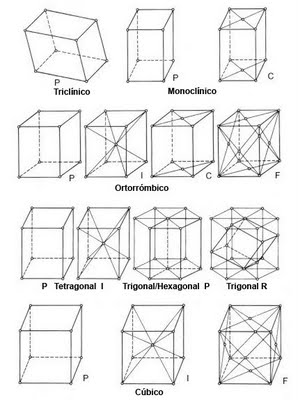
\includegraphics[scale=1]{Bravais.jpg}
					\caption{Redes de Bravais}
				\end{center}			
			\end{figure}
	
	\chapter{Electrones en metales}	
		\section{Teoría clásica de Drude-Lorentz de los electrones libres}	
		
			El modelo de Drude-Lorentz aplica la teoría cinética	para tratar de explicar las propiedades de los metales.Para ello considera que los electrones de valencia se mueven libremente, sin ser afectados por el potencial iónico de la red, dentro del metal y por tanto pueden ser modelados como un gas clásico.Drude supuso que la carga positiva que compensa a los electrones estaba ligada a partículas mucho más pesadas (iones), las cuales  él las considera inmóviles
		
			Se impone como hipótesis:\\
			
			\begin{itemize}
				\item Entre dos colisiones, los electrones de conducción se mueven libremente.
				\item Se desprecian las interacciones electrón–electrón (aproximación de \textbf{electrones independientes}).
				\item Se desprecian las interacciones Coulombianas electrón-ión (aproximación de \textbf{electrones libres}).
				\item Las colisiones con los iones son eventos instantáneos que cambian abruptamente la velocidad de los electrones.
				\item El tiempo medio entre colisiones es $\tau$, es decir, un electrón choca con probabilidad $1/\tau$ por unidad de tiempo. El tiempo $\tau$ se conoce como: \textbf{tiempo de relajación}, tiempo de colisión o tiempo libre medio.
				\item Los electrones alcanzan un \textbf{equilibrio térmico} con su entorno sólo a través de colisiones, donde el electrón emerge con una velocidad cuya dirección es aleatoria y con una magnitud dada por la temperatura reinante en el lugar de la colisión.
				\item Los electrones de valencia, constituyendo un gas ideal clásico, responden a la \textbf{estadística de Maxwell-Boltzmann}.
			\end{itemize}					

			\subsection{Velocidad térmica y de desplazamiento debido a campo eléctrico}
			
				Se tiene un cable de largo $L$ y sección $A$ al que se le aplica una diferencia de potencial en sus extremos. La corriente circulante por la sección puede tomarse como una densidad de corriente $\vec{J}$ tal que $\vec{I}=\vec{J}A$. la diferencia de potencial aplicada a ambos extremos del cable cumple $\Delta V= |\vec{E}| L$. El cable presenta una resistividad eléctrica $\rho$ que relaciona al campo eléctrico con la densidad de corriente ($\vec{E}=\rho \vec{J}$), de donde se puede obtener la \textbf{Ley de Ohm}: \boxed{\vec{J}=\sigma \vec{E}}, con $\sigma=1/\rho$ como la conductividad eléctrica del material.\\
				
				Para obtener $\sigma$ dentro del modelo de Drude se tomará $n$ como el número de electrones por $cm^3$ y $\langle \vec{v} \rangle$ la velocidad promedio con que los electrones avanzan en un metal. Sea $t$ el tiempo que ha transcurrido desde la última colisión, para un electrón
determinado. Su velocidad será:

				\begin{center}
					$\displaystyle \vec{v}(t)=\vec{v}_0+(-e)\vec{E}t\frac{1}{m} \Rightarrow \langle \vec{v}(t) \rangle=\underbrace{\langle \vec{v}_0 \rangle}_{0}+\underbrace{\langle(-e)\vec{E}t\frac{1}{m} \rangle}_{\langle t \rangle=\tau} \Rightarrow$ \boxed{\displaystyle \langle \vec{v}(t) \rangle=-\frac{e|\vec{E}|\tau}{m}}\\
				\end{center}

				Debido a que las velocidades se distribuyen aleatoriamente después de una colisión. Entonces como la densidad de corriente es la cantidad de electrones que atraviesan el cable por unidad de área y tiempo:\\
				
				\begin{center}
					$\displaystyle \vec{J}=-n e \langle \vec{v}(t) \rangle=\left( \frac{n e^2 \tau}{m}\right) \vec{E}  \Rightarrow$ \boxed{\displaystyle \sigma=\frac{n e^2 \tau}{m}}
				\end{center}
				
			\subsection{Tiempo de relajación}
			
				Se puede obtener el tiempo de relajación de $\displaystyle \sigma=\frac{n e^2 \tau}{m}$, entonces \boxed{\displaystyle \tau=\frac{m \sigma}{n e^2}=\frac{m}{n e^2 \rho}}
						
			\subsection{Camino libre medio}
			
				Se define el camino libre medio $\lambda$, con $\langle \vec{v} \rangle$ la velocidad media, como:
				
				\begin{center}
					$\lambda=\langle \vec{v} \rangle \tau$
				\end{center}		
			
				Por el teorema de equipartición de la energía: $\langle \vec{E} \rangle=\frac{1}{2}m\langle \vec{v} \rangle^2=\frac{3}{2}k T$, con k la constante de Boltzmann.
				
				\begin{center}
					$\displaystyle \langle \vec{v} \rangle =\sqrt{\frac{3 k T}{m}} \Rightarrow$ \boxed{\lambda=\sqrt{\frac{3 k T}{m}} \frac{m}{n e \rho^2}=\frac{-e|\vec{E}|}{m}\tau^2}
				\end{center}
			
			\subsection{Movilidad}
			
				La movilidad electrónica $\mu$ es la medida de la facilidad con que un electrón se mueve por acción de un campo eléctrico:
				
				\begin{center}
					$\displaystyle \langle \vec{v}(t) \rangle=-\frac{e\vec{E}\tau}{m} \Rightarrow \langle \vec{v}(t) \rangle=-\mu \vec{E} \Rightarrow $ \boxed{\displaystyle \mu=\frac{e\tau}{m}}
				\end{center}
						
			\subsection{Conductividad}
			
			\begin{center}
				$\displaystyle \sigma=n e \mu=\frac{n e^2 \tau}{m}$
			\end{center}
			
			El modelo es consistente con la Ley de Ohm y puede dar una explicación de la resistencia eléctrica.\\
			
			\subsection{Capacidad calorífica}

				Si se calcula que cada elecron tiene una energía cinética media $\langle E_c \rangle_{MB}=\frac{3}{2}kT$, entonces:\\
				 $C_{v_e}=\frac{d U}{dT}=\frac{3}{2}Nk$, pero las mediciones dan resultados muchos menores. El aporte de los electrones a la capacidad calorífica es una falla del modelo.
			
		\section{Fallas de la teoría clásica}	
		
			\begin{enumerate}
				\item La suposición que el camino libre medio $\lambda$ es del orden de la constante de red no es verificada por los valores medidos de $\lambda$ los cuales son mucho más grandes.
				\item La parte electrónica de la capacidad calorífica no es explicada correctamente.
				\item La dispersión de los electrones con los iones es el proceso dominante en el modelo: a temperaturas más grandes, vibraciones más fuertes de los iones y dispersiones más fuertes (dispersión de fonones)
			\end{enumerate}					
			
		\section{Teoría cuántica de Sommerfeld}	
		
			Sommerfeld propone las siguientes hipótesis:
			
			\begin{itemize}
				\item Aproximamos el potencial real en un cristal por un \textbf{pozo de potencial infinito}.
				\item El potencial infinito en los bordes previene el escape de electronesnes (experimentalmente, corresponde a la \textbf{función trabajo} de los electrones)
				\item Llamaremos gas de electrones libres de Fermi a un gas que obedece la \textbf{estadística de Fermi-Dirac} y el \textbf{principio de exclusión} de Pauli.
				\item En mecánica cuántica los electrones obedecen a la \textbf{ecuación de Schröndinger}.	
		
		\end{itemize}	
		
			\subsection{Aplicaciones de la estadística de Fermi-Dirac}
			
				La función de distribución de Fermi-Dirac establece la probabilidad de que un electrón ocupe el estado de energía $\varepsilon$ a la temperatura $T$. La misma es complicada de utilizar en los cálculos, por lo que se la suele aproximar, a temperaturas menores a $T_f$ por el escalón unitario hasta la energía de Fermi y luego la función nula. Esto facilita enormemente los cálculos, sin pérdida significativa de generalidad ni exactitud.
			
			\subsection{Nivel de Fermi en un metal}		
			
				Definimos la energía de Fermi $\varepsilon_f$ como la energía del nivel ocupado más alto. Resolviendo la ecuación de Schrödinger se encuentra que:\\
				
				\begin{center}
					$\displaystyle -\frac{\hbar^2}{2m}\nabla^2\Psi_{\vec{k}}=\varepsilon_{\vec{k}}\Psi_{\vec{k}} \Rightarrow \Psi_{\vec{k}}(\vec{r})=A e^{j\vec{k}\vec{r}} \Rightarrow \varepsilon_{\vec{k}}=\frac{\hbar^2 k^2}{2m} $
				\end{center}
				
				Particularmente para $k=k_f$ se tiene que $\displaystyle \varepsilon_f=\frac{\hbar^2}{2m}k_f^2$. Ya se había calculado la energía de Fermi para un espacio tridimensional, usando ese dato se puede despejar el número de onda $k_f$:\\
				
				\begin{center}
					$\displaystyle \varepsilon_f(T=0K)=\frac{h^2}{8m}\left(\frac{3}{\pi}\frac{N}{V}\right)^{\frac{2}{3}}=\frac{h^2}{8 \pi^2 m}k_f^2 \Rightarrow k_f=\left(\frac{3N\pi^2}{V}\right)^{\frac{1}{3}}$
				\end{center}
				
				\subsubsection{Cálculo y variación térmica}
				
					Considerando un sistema aislado, con un número de partículas constante y termodinámicamente en equilibrio. Se tiene:\\
					
					\begin{enumerate}
						\item $n(\varepsilon)d\varepsilon=g(\varepsilon)F_{FD}(\varepsilon)d\varepsilon$
						\item $\displaystyle F_{FD}(\varepsilon)=\frac{1}{e^{\frac{\varepsilon-\varepsilon_f}{kT}}+1}$
						\item $\displaystyle g(\varepsilon)=\frac{3}{2}N \varepsilon_f^{-3/2}\varepsilon^{1/2} \Rightarrow g(\varepsilon)=\frac{\pi}{2}\left(\frac{8mL^2}{h^2}\right)^{3/2} \varepsilon^{1/2}$\\
						$\displaystyle N=\int_0^{+\infty} n(\varepsilon)d\varepsilon=\int_0^{+\infty} g(\varepsilon)F_{FD}(\varepsilon)d\varepsilon=\int_0^{+\infty}\frac{\pi}{2}\left(\frac{8mL^2}{h^2}\right)^{3/2} \varepsilon^{1/2} F_{FD}(\varepsilon)d\varepsilon=\frac{4\pi V(2m)^{3/2}}{h^3}\underbrace{\int_0^{+\infty} \frac{\varepsilon^{1/2}}{e^{\frac{\varepsilon-\varepsilon_f}{kT}}+1}d\varepsilon}_{(4)}$\\
						\item $\displaystyle \int_0^{+\infty} \frac{\varepsilon^{1/2}}{e^{\frac{\varepsilon-\varepsilon_f}{kT}}+1}d\varepsilon \simeq \frac{2}{3}\varepsilon_f^{3/2}\left[1+(kT)^2\frac{\pi}{8}\varepsilon_f^{-2} \right] \Rightarrow N \simeq \frac{4\pi V(2m)^{3/2}}{h^3}\frac{2}{3}\varepsilon_f^{3/2}\left[1+(kT)^2\frac{\pi}{8}\varepsilon_f^{-2} \right]$
						\item $\displaystyle \varepsilon_f=\underbrace{\frac{h^2}{8m}\left(\frac{3}{\pi}\frac{N}{V}\right)^{\frac{2}{3}}}_{\varepsilon_f(T=0K)}\left[1+\frac{\pi^2}{8}\left(\frac{kT}{\varepsilon_f}\right)^2\right]^{-2/3} \Rightarrow \varepsilon_f=\varepsilon_f(T=0K)\left[1+\frac{\pi^2}{8}\left(\frac{kT}{\varepsilon_f}\right)^2\right]^{-2/3}$		
						\item Considero $\frac{kT}{\varepsilon_f} \approx 0$ y desarrollo en serie a primer orden $(1+x)^{-2/3}=1-\frac{2}{3}x$: \boxed{\varepsilon_f=\varepsilon_f(T=0K)\left[1-\frac{\pi^2}{12}\left(\frac{kT}{\varepsilon_f}\right)^2\right]}					
					\end{enumerate}
													
			\subsection{Transporte de carga}
			
				\begin{itemize}
					\item Densidad de corriente: $\displaystyle \vec{J}=-ne \langle \vec{v}(t) \rangle=\frac{n e^2 \tau}{m}\vec{E}$
					\item Conductividad: $\displaystyle \sigma=\frac{n e^2 \tau}{m}=ne\mu=\frac{1}{\rho}$
					\item Resistividad $\rho$ debido a la difusión cuya rapidez es proporcional a $1/\tau$
					\item El tiempo de vida medio se debe a dos mecanismos de dispersión:
						\begin{enumerate}
							\item Dispersión con los iones: La vibración de los iones genera fonones(cuantos de vibración) de energía proporcional a $\hbar \omega(n_x+n_y+n_z+3/2)$, con densidad de fonones en función de la temperatura. Cada electrón interactúa con los fonones, a más fonones, mas colisiones con los electrones.
							\item Imperfecciones de la red cristalina: Falta de iones en una posición dada, contaminación con impurezas o desplazamiento de planos atómicos.
						\end{enumerate}
					\item Ley de Matthiessen: $\displaystyle \rho_{total}(T)=\underbrace{\rho(T)}_{\text{Fonón}}+\underbrace{\rho_0}_{\text{cristal}} \propto \frac{1}{\tau_{\text{Fonón}}(T)}+\frac{1}{\tau_{cristal}}$					
				\end{itemize}
			
		\section{Calor específico de un gas de electrones}
		
			\begin{itemize}
				\item \textbf{Calor específico debido a los fonones:} Interpretando al sólido cristalino con la distribución de Maxwell-Boltzman, existen $N_0$, el número de Avogadro, átomos en un mol. Se considera que cada átomo lleva a cabo oscilaciones armónico-simples en torno a su posición en la red, en tres dimensiones. Cada mol tiene $3N_0$ grados de libertad, a cada uno se le asigna una energía total promedio $kT$, de acuerdo con la ley clásica de la equipartición de la energía:   $\varepsilon=3 N_0 kT=3RT$, donde $R$ es la constante universal de los gases:
			
				\begin{center}
					$\displaystyle C_v^{red}=\frac{d\varepsilon}{dT}=3R$ : Ley de Bulong y Petit
				\end{center}		
		
				Pero experimentos posteriores mostraron que a menor temperatura las capacidades caloríficas varían. Einstein corrigió el problema tomando en cuenta la cuantización de la energía en un oscilador armónico simple:
			
				\begin{center}
					$\displaystyle \varepsilon=\frac{3N_0 h \nu}{e^{\frac{h \nu}{kT}}-1}=3RT\frac{\frac{h \nu}{kT}}{e^{\frac{h \nu}{kT}}-1}$
				\end{center}
		
				Pero aunque encontró una concordancia cualitativa con los resultados experimentales a temperaturas razonablemente bajas, debe escogerse una frecuencia característica $\nu$ diferente para cada sustancia y a temperaturas muy bajas no contiene la dependencia con la temperatura $T^3$ que requieren los resultados experimentales.\\
			
				El error se encuentra en suponer que los átomos del sólido vibran independientemente entre sí, en realidad están fuertemente acoplados. Debye hizo ver que una superposición de modos elásticos de vibración longitudinal del sólido como un todo proporciona los mismos movimientos atómicos individuales que el acoplamiento real. Las vibraciones térmicas de los átomos del sólido son equivalentes a una combinación grande de ondas elásticas estacionarias en un gran intervalo de frecuencias, donde cada modo se puede considerar como un oscilador armónico independiente, de eigenvalores cuantizados conocidos. Entonces,sumando se puede obtener la energía total del sistema.\\
			
				La distribuación de Maxwell-Boltzmann sigue siendo válida ya que los átomos individuales se pueden considerar como partículas distinguibles, debido a su posición en el espacio en los sitios de la red del cristal. Además que la sustitución propuesta por Debye garantiza que serán elementos independientes sin interacción entre sí. Cada modo de vibración está caracterizado por un conjunto diferente de números ($n_x$,$n_y$,$n_z$).\\
			
				Número de modos con frecuencias entre $\nu$ y $\nu+\delta \nu$ es: $\displaystyle N(\nu)d\nu=\frac{4\pi V}{\upsilon^3}\nu^2d\nu$, con $\upsilon$ la velocidad de ondas elásticas y $V$ el volumen del sólido. Debye supuso que el número de modos está limitado a $3 N_0$ por mol:\\
			
				\begin{center}
					$\displaystyle \int_0^{\nu_{max}} N(\nu)d\nu=3 N_0=\frac{4\pi V}{3\upsilon^3} \nu_{max}^3 \Rightarrow \nu_{max}=\upsilon\left(\frac{9 N_0}{4\pi V} \right)^{1/3}$
				\end{center}
		
				La energía elástica total será: $\displaystyle \varepsilon=\int_0^{\nu_{max}}\frac{h\nu}{e^{\frac{h\nu}{kT}}-1}\frac{4\pi V}{\upsilon^3}\nu^2 d\nu$. Aplicando el cambio de variable $x=\frac{h\nu}{kT}$:\\
		
				\begin{center}
					$\displaystyle \varepsilon=\frac{4\pi V}{\upsilon^3}\left(\frac{kT}{h}\right)^4 h \int_0^{x_{max}}\frac{x^3dx}{e^x-1}$
				\end{center}		
		
				Se sustituye $\displaystyle \frac{4\pi V}{\upsilon^3}=\frac{9 N_0}{\nu_{max}^3}$ y se obtiene la fórmula de Debye: $\displaystyle \varepsilon=3RT\frac{3}{x_{max}^3} \int_0^{x_{max}}\frac{x^3dx}{e^x-1}$.\\
		
				Como $x$ es una cantidad adimensional, entonces $h\nu_{max}/k$ tiene las dimensiones de temperatura y se conoce como temperatura de Debye, $\Theta$. Podemos escribir $\displaystyle x_{max}=\frac{\Theta}{T}$:
		
				\begin{center}
					$\displaystyle \varepsilon=9R\frac{T^4}{\Theta^3}\int_0^{\Theta/T} \frac{x^3}{e^x-1}dx$
				\end{center}
		
				La fórmula de Debye para el calor específico de un sólido es:
			
				\begin{center}
					$\displaystyle C_v^{red}=\frac{d\varepsilon}{dT}=9R\left[4\left(\frac{T}{\Theta}\right)^3\int_0^{\Theta/T} \frac{x^3}{e^x-1}dx-\frac{\Theta}{T}\frac{1}{e^{\Theta/T}-1}\right]$
				\end{center}
		
				A temperaturas bajas se tiene:
			
				\begin{center}
					$\displaystyle \lim_{T \to 0} C_v^{red}=\lim_{T \to 0} 9R\left[4\left(\frac{T}{\Theta}\right)^3\int_0^{\Theta/T} \frac{x^3}{e^x-1}dx-\frac{\Theta}{T}\frac{1}{e^{\Theta/T}-1}\right]=9R4\left(\frac{T}{\Theta}\right)^3 \underbrace{\int_0^{\infty} \frac{x^3}{e^x-1}dx}_{\frac{\pi^4}{15}} \Rightarrow$
				\end{center}
		
				\begin{center}
					\boxed{\displaystyle C_v^{red}=\frac{12\pi^4}{5}\frac{R}{\Theta^3}T^3}
				\end{center}
		
				\item \textbf{Calor específico debido a los electrones:}\\
				
				\begin{center}
					$\displaystyle U=\int_0^{\infty} \varepsilon g(\varepsilon)F_{FD}(\varepsilon) d\varepsilon \Rightarrow C_v^{e^-}=\left( \frac{\partial U}{\partial T}\right)_V=\int_0^{\infty} \varepsilon g(\varepsilon)\left(\frac{\partial F_{FD}(\varepsilon)}{\partial T}\right)_V d\varepsilon$
				\end{center}
				
				\begin{center}
					$\displaystyle C_v^{e^-}=k^2T g(\varepsilon_f)\int_0^{\infty} \left(\frac{\varepsilon-\varepsilon_f}{kT}\right)^2 g(\varepsilon)\frac{e^{\frac{\varepsilon-\varepsilon_f}{kT}}}{\left(e^{\frac{\varepsilon-\varepsilon_f}{kT}}+1\right)^2} \frac{d\varepsilon}{kT}$
				\end{center}
		
				Haciendo el cambio de variable $x=\frac{\varepsilon-\varepsilon_f}{kT} \Rightarrow dx=\frac{d\varepsilon}{kT}$:
				
				\begin{center}
					$\displaystyle C_v^{e^-} \approx g(\varepsilon_f)k^2T\int_{-\frac{\epsilon_f}{kT}}^{\infty} \frac{e^x x^2 dx}{(e^x+1)^2} \underbrace{\longrightarrow}_{-\frac{\epsilon_f}{kT} \gg 1} C_v^{e^-} \approx g(\varepsilon_f)k^2T\underbrace{\int_{-\infty}^{\infty} \frac{e^x x^2 dx}{(e^x+1)^2}}_{\pi^2/3}$
				\end{center}
			
				\begin{center}
					$\displaystyle C_v^{e^-} \approx \frac{g(\varepsilon_f)k^2T\pi^2}{3}=\frac{k^2T\pi^2}{3}\left(\frac{V(2m)^{3/2}}{2\pi^2 \hbar^3} \right)\varepsilon_f^{1/2}=\frac{k^2T}{6}V\left(\frac{2m}{\hbar^2}\right)^{3/2}\varepsilon_f^{1/2}$
				\end{center}

				\begin{center}
					$\displaystyle C_v^{e^-} \approx \frac{k^2T}{6}V\left(\frac{3\pi^2N}{V \varepsilon_f}\right)=\frac{k^2T}{2}\left(\frac{\pi^2N}{k T_f}\right)$
				\end{center}
				
				\begin{center}
					\boxed{\displaystyle C_v^{e^-}=\frac{\pi^2kN}{2}\left(\frac{T}{T_f}\right)=\gamma T}
				\end{center}
				
			\end{itemize}
			\subsection{Aporte al calor específico de un sólido}
			
				El calor específico del sólido será:
				
				\begin{center}
					$\displaystyle C_v^{\text{sólido}}=\underbrace{C_v^{red}}_{\text{fonónes}}+\underbrace{C_v^{e^-}}_{\text{electrones}}=\frac{12\pi^4}{5}\frac{R}{\Theta^3}T^3+\frac{\pi^2kN}{2}\left(\frac{T}{T_f}\right)$
				\end{center}
			
				A temperatura ambiente, la contribución al calor específico de los electrones es despreciable.\\
				
				A bajas temperaturas, donde las vibraciones de la red llegan a ser pequeñas, la contribución de los electrones pueden llegar a ser importantes.
				
	\chapter{Teoría de bandas}

		\section{Teoría cuántica de electrones en redes periódicas}
	
			\subsection{Teorema de Bloch}
			
				Consideremos un electrón moviéndose en un potencial periódico \boxed{U(\vec{r}+\vec{R})=U(\vec{r})}, $\forall \vec{R} \in{\text{Red de Bravais}}$ y la ecuación de Schrödinger independiente del tiempo :$\displaystyle \hat{H}\Psi(\vec{r})=\left[-\frac{\hbar^2}{2m}\nabla^2+U(\vec{r})\right]\Psi(\vec{r})=\varepsilon \Psi(\vec{r})$.\\
				
				El teorema de Bloch establece que las autofunciones de un Hamiltoniano con potencial periódico se pueden elegir de tal manera que:
				
				\begin{center}
					\boxed{\displaystyle \Psi(\vec{r}+\vec{R})=e^{i\vec{K}\vec{R}}\Psi(\vec{r})}
				\end{center}
				
				Donde $\vec{K}$ es el vector de onda de Bloch o vector de onda cristalino. La función de onda puede escribirse de la forma:
				
				\begin{center}
					\boxed{\displaystyle \Psi(\vec{r})=e^{i\vec{K}\vec{r}}\mu_{\vec{K}}(\vec{r})}\\
					$\Downarrow$\\
					$\displaystyle \Psi(\vec{r}+\vec{R})=e^{i\vec{K}\vec{R}}\Psi(\vec{r})=e^{i\vec{K}\vec{R}}e^{i\vec{K}\vec{r}}\mu_{\vec{K}}(\vec{r})$\\
					$\Downarrow$\\
					Por otra parte\\
					$\Downarrow$\\
					$\displaystyle \Psi(\vec{r}+\vec{R})=e^{i\vec{K}(\vec{R}+\vec{r})}\mu_{\vec{K}}(\vec{r}+\vec{R})$\\
					$\Downarrow$\\
					\boxed{\displaystyle \mu_{\vec{K}}(\vec{r}+\vec{R})=\mu_{\vec{K}}(\vec{r})} $\text{  } \forall \vec{R} \in{\text{Red de Bravais}}$ 
				\end{center}
			
			\subsection{Condiciones de contorno periódicas}
			
				Las condiciones de borde periódicas, o de Born von Karman, que piden que no exista función de onda en los bordes del cristal, son ciertas si el cristal es infinito, pero tener un cristal finito con condiciones de borde cíclicas es similar a tener un cristal infinito.\\
				
				Sean $\vec{a}_1$,$\vec{a}_2$,$\vec{a}_3$ vectores primitivos, definimos $N \equiv N_1 N_2 N_3$ y sean $N_1 \vec{a}_1$,$N_2 \vec{a}_2$,$N_3 \vec{a}_3$ los lados de una celda unitaria. Aplicando las condiciones de borde de Born Von Karman:
				
				\begin{center}
					$\displaystyle \Psi(\vec{r}+N_i \vec{a}_i)=\Psi(\vec{r}) \text{  ,   } i=1,2,3.$\\
					$\Downarrow$\\				
					$\displaystyle \Psi(\vec{r}+N_i \vec{a}_i)=\underbrace{e^{i \vec{K} N_i \vec{a}_i}}_1 \Psi(\vec{r}) \text{  ,   } i=1,2,3.$\\
					$\Downarrow$\\
					$\displaystyle N_i \vec{K} \vec{a}_i=2\pi n_i \text{ , } n_i \in{Z}$
					$\Downarrow$\\
					$\displaystyle \vec{K}=\sum_{j=1}^3 \frac{n_j}{N_j}\vec{a^*}_j \text{ , con } \vec{a}_i \cdot \vec{a}_j=2\pi \delta{i j}$
				\end{center}
			
			\subsection{Modelo de Kronig-Penney en cristal unidimensional infinito}
			
				Kronig y Penney plantean un modelo matemático de potencial iónico periódico, que permite describir el comportamiento de los electrones dentro de un cristal.\\
				
				El modelo considera a un único electrón desplazándose a través de la red, de tal manera que en la energía potencial, $E(x)$, es nulo en las
regiones del tipo I y $E_0$ en las de tipo II. Los iones se ubican en las regiones del tipo I y la separación entre los mismos (L, que representa el parámetro de red) genera una barrera de potencial para los electrones.
			
				\begin{figure}[H]
					\begin{center}
						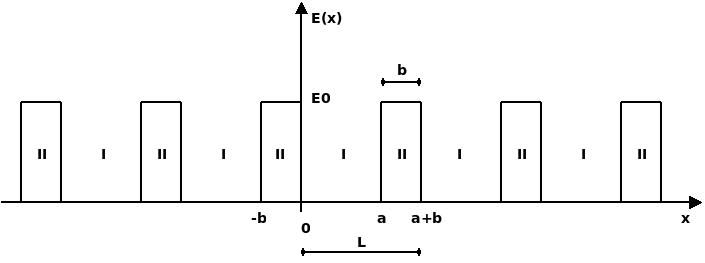
\includegraphics[scale=0.7]{Penney.jpeg}
						\caption{Modelo de potencial periódico de Kronig-Penney}
					\end{center}					
				\end{figure}	
			
			El movimiento de la partícula esta determinado por la ecuación de Schrödinger independiente del tiempo:
			
			\begin{center}
				$\displaystyle (E(x)-E_0)\Psi(x)=\frac{\hbar^2}{2m}\frac{\partial \Psi(x)}{\partial x^2}$
			\end{center}
			
			Donde $E_0$ es la energía mecánica total del electrón. La solución de la ecuación es una función de onda de Bloch:
			
			\begin{center}
				$\displaystyle \Psi(x)=\mu(x)e^{i K x}$
			\end{center}
			
			Donde $\mu(x)$ es la amplitud con el período de la red L. La forma de la amplitud $\mu(x)$ y los valores permitidos de $K$ son los que deberán determinarse.\\
			
			\begin{minipage}[t]{0.5\textwidth}
				\begin{center}
					Región I($E(x)=0$):\\
				\end{center}
				\begin{center}
					$\displaystyle \frac{\partial^2 \Psi(x)}{\partial x^2}=-\underbrace{\frac{2mE}{\hbar^2}}_{\alpha^2}\Psi(x)$\\
					$\Downarrow$\\
					$\displaystyle \frac{\partial^2 \Psi(x)}{\partial x^2}=-\alpha^2 \mu_1(x) e^{i K x}$\\
					$\Downarrow$\\
					$\displaystyle \left[\frac{\partial^2 \mu_1(x)}{\partial x^2}+2iK\frac{\partial \mu_1(x)}{\partial x}-(K^2-\alpha^2)\mu_1(x)\right]e^{i K x}=0$\\			
				\end{center}
			\end{minipage}
			\begin{minipage}[t]{0.5\textwidth}
				\begin{center}
					Región II($E(x)=E_0$):\\
				\end{center}
				\begin{center}
					$\displaystyle \frac{\partial^2 \Psi(x)}{\partial x^2}=\underbrace{-\frac{2m(E-E_0)}{\hbar^2}}_{\beta^2}\Psi(x)$\\
					$\Downarrow$\\
					$\displaystyle \frac{\partial^2 \Psi(x)}{\partial x^2}=\beta^2 \mu_2(x) e^{i K x}$\\
					$\Downarrow$\\
					$\displaystyle \left[\frac{\partial^2 \mu_2(x)}{\partial x^2}+2iK\frac{\partial \mu_2(x)}{\partial x}-(K^2+\beta^2)\mu_2(x)\right]e^{i K x}=0$\\
				\end{center}
			\end{minipage}
			
			\vfill
			La solución de ambas ecuaciones tendrá la forma:
			
				\begin{center}
					$\displaystyle \mu_1(x)=A e^{j(\alpha-K)x}+B e^{-j(\beta+K)x}$
				\end{center}
				\begin{center}
					$\displaystyle \mu_2(x)=C e^{j(\alpha-K)x}+D e^{-j(\beta+K)x}$
				\end{center}
			
			Las mismas deberán cumplir las condiciones de continuidad en los límites de las regiones y sus derivadas.
			
			\begin{minipage}[t]{0.5\textwidth}
				\begin{center}
					$x=0$:\\
				\end{center}
				\begin{center}
					$\displaystyle \mu_1(0)=\mu_2(0)$\\		
				\end{center}
				\begin{center}
					$\displaystyle \left(\frac{d\mu_1(x)}{dx}\right)_{x=0}=\left(\frac{d\mu_2(x)}{dx}\right)_{x=0}$\\		
				\end{center}
			\end{minipage}
			\begin{minipage}[t]{0.5\textwidth}
				\begin{flushleft}
					$x=-b$ y $x=a$:\\
				\end{flushleft}
				\begin{flushleft}
					$\displaystyle \mu_1(a)=\mu_2(-b)$\\		
				\end{flushleft}
				\begin{flushleft}
					$\displaystyle \left(\frac{d\mu_1(x)}{dx}\right)_{x=a}=\left(\frac{d\mu_2(x)}{dx}\right)_{x=-b}$\\		
				\end{flushleft}
			\end{minipage}
	
			\subsection{Bandas de energía prohibidas}
			
				Resolviendo el sistema de 4 ecuaciones con 4 incognitas:
				
				\begin{center}
					$\displaystyle \frac{\beta^2-\alpha^2}{2\alpha\beta}\sinh(\beta b)\sin(\alpha a)+\cosh(\beta b)\cos(\alpha a)=\cos[K(a+b)] \text{ con } K=\frac{2\pi n}{N(a+b)}$
				\end{center}
							
				Siendo	$N$ el número de átomos. El primer miembro es una relación trigonométrica y el segundo es una función armónica válida entre $-1$ y $+1$\\
				
				La resolución numérica de la ecuación de Kronig-Penney prueba la formación de:
				
				\begin{itemize}		
					\item Bandas de energía permitidas, donde los valores energéticos son permitidos.
					\item Bandas de energía prohibidas, donde no son permitidos los valores energéticos.								
				\end{itemize}											
							
				\begin{figure}[H]
					\begin{center}
						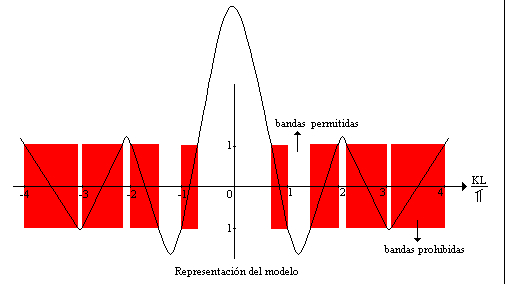
\includegraphics[scale=1]{KP.jpg}
						\caption{Modelo de potencial periódico de Kronig-Penney}
					\end{center}					
				\end{figure}		
			
			\subsection{Energía en función del número de onda del Modelo de Kronig-Penney}
			
			Se considera un cristal unidimensional que es tan largo que se pueden ignorar las condiciones a la frontera en sus extremos. Las autofunciones más convenientes para un electrón libre, son ondas viajeras senoidales del tipo $\Psi(x) \propto e^{\pm i k x}$. Aunque es mas conveniente tomar una sola dirección, $k$ puede ser positiva o negativa. Se puede escribir la energía $\varepsilon$ de un electrón libre en términos de su número de onda $k=p/\hbar$, donde $p$ es su impulso:
			
			\begin{center}
				\boxed{\displaystyle \varepsilon=\frac{p^2}{2m}=\frac{\hbar^2k^2}{2m}}
			\end{center}
		
			\subsection{Representación en zona reducida}
			
				\begin{figure}[H]
					\begin{center}
						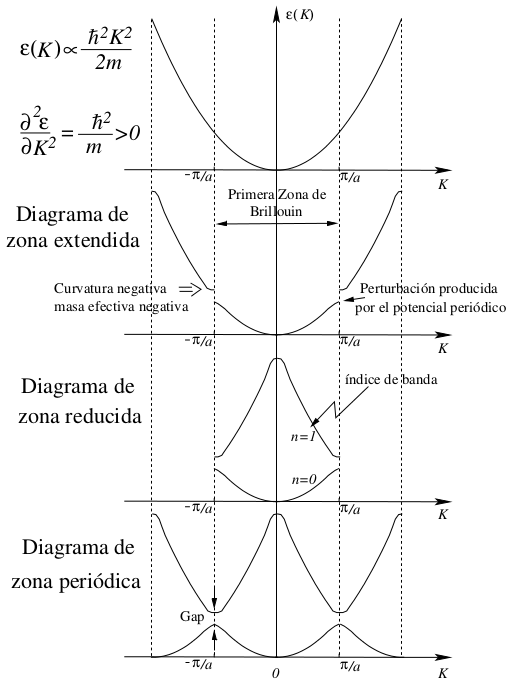
\includegraphics[scale=0.7]{Bloch.png}
						 \caption{Energías permitidas}
					\end{center}					
				\end{figure}							
			
			\subsection{Número de estados en una banda}
			
				Tomando la distribución de energías de los electrones como un producto de la densidad de estados $N(\varepsilon)$ y la distribuación de Fermi $F_{FD}(\varepsilon)$ que sea apropiada en las bandas de valencia, prohibidas y de conducción de un aislante. Si $\varepsilon-\varepsilon_f \gg kT$ entonces:
				
				\begin{center}
					$\displaystyle F_{FD}(\varepsilon)=\frac{1}{e^{\frac{\varepsilon-\varepsilon_f}{kT}}+1} \simeq e^{-\left(\frac{\varepsilon-\varepsilon_f}{kT}\right)}$
				\end{center}
			
				De modo que en ese intervalo de energías, la distribución de Fermi varía con la energía, como la distribución de Boltzmann. En el fondo de la banda de conducción de un aislante, si $\varepsilon$ se mide de la parte superior de la banda de valencia, entonces $\displaystyle \varepsilon-\varepsilon_f=\frac{\varepsilon_{gap}}{2}$. Como $\varepsilon_{gap} \gg kT$ para un aislante, se cumple la condición $\varepsilon-\varepsilon_f \gg kT$ y se puede tomar:
				
				\begin{center}
					$\displaystyle F_{FD}(\varepsilon)=e^{-\left(\frac{\varepsilon_{gap}}{2kT}\right)}$
				\end{center}
						
				Como el número de electrones por estado en la banda de conducción de un aislante.\\
				
				La distribución de Fermi decae en su valor por un orden de magnitud, en un intervalo de energías de aproximadamente $\Delta \varepsilon=2kT$ de modo que se puede obtener una buena aproximación de $\Delta N$, el número de electrones de conducción, calculando los que se encuentran en un intervalo de $2kT$ por encima del fondo de la banda de conducción.\\
				
				Como $\Delta N=F_{FD}(\varepsilon)N(\varepsilon) \Delta \varepsilon$ enseguida debe evaluarse $N(\varepsilon)$, la densidad de estados. Dado que $N(\varepsilon)$ empieza en cero, en el fondo de la banda de conducción, se obtiene un buen valor promedio sobre el intervalo $\Delta \varepsilon=2kT$, evaluando $N(\varepsilon)$ cuando $\varepsilon=kT$. Por tanto:
				
				\begin{center}
					$\Delta N=F_{FD}(\varepsilon)N(\varepsilon) \Delta \varepsilon=e^{-\left(\frac{\varepsilon_{gap}}{2kT}\right)}N(kT)2kT$
				\end{center}
			
				Utilizando que $\displaystyle N=\frac{2}{3}\varepsilon_f N(\varepsilon)$ y $\displaystyle \frac{N(kT)}{N(\varepsilon_f)}=\sqrt{\frac{kT}{\varepsilon_f}}$ se obtiene:
				
				\begin{center}
					$\displaystyle \frac{\Delta N}{N} \simeq \frac{e^{-\left(\frac{\varepsilon_{gap}}{2kT}\right)} N(kT)2kT}{\frac{2}{3}\varepsilon_f N(\varepsilon_f)}=3e^{-\left(\frac{\varepsilon_{gap}}{2kT}\right)}\left(\frac{kT}{\varepsilon_f}\right)\sqrt{\frac{kT}{\varepsilon_f}}$
				\end{center}
				\begin{center}
					\boxed{\displaystyle \frac{\Delta N}{N} \simeq \left(\frac{kT}{\varepsilon_f}\right)^{\frac{3}{2}}e^{-\left(\frac{\varepsilon_{gap}}{2kT}\right)}}
				\end{center}
			
				Este es el número relativo de electrones de conducción para un aislante.\\
			
		\section{Dinámica de electrones en redes cristalinas unidimensionales}

			Al estudiar el comportamiento de un electrón en una red periódica bajo la influencia de un campo eléctrico externo, es muy conveniente introducir el concepto de \textbf{masa efectiva} del electrón, describiendo el movimiento del electrón en términos de un grupo de ondas viajeras.		
		
			\subsection{Velocidad de grupo}
			
				Se define a la velocidad de grupo como la derivada de las frecuencias $\nu$ de las ondas viajeras senoidales componentes, con respecto a sus longitudes de onda recíprocas $\kappa$
				
				\begin{center}
					$\displaystyle v_{grupo}=\frac{d \nu}{d \kappa}=\frac{d\omega}{dk}=\frac{1}{\hbar}\frac{d\varepsilon}{dk}=\frac{d}{dk}\left(\frac{\hbar k^2}{2m}\right)=\frac{\hbar k}{m}=\frac{p}{m}=\frac{mv}{m}=v$	
				\end{center}		
			
			La velocidad de grupo es igual a la velocidad del electrón cuyo movimiento está representado por el grupo.
			
			\subsection{Masa efectiva}
			
				Se considera un electrón en una red unidimensional, cuyo número de onda depende de la energía en la forma $\varepsilon(k)$ y se le aplica un campo eléctrico externo $\vec{E}$. En un tiempo $dt$, el electrón de carga $q$ se mueve una distancia $dx$. Como ésto es igual a la magnitud del cambio en la energía del electrón $d\varepsilon$, se obtiene:
				
				\begin{center}
					$\displaystyle d\varepsilon=q E dx=q E \frac{dx}{dt}dt=q E v dt=q E v_{grupo} dt$\\
				\end{center}
				
				Y como $\varepsilon=\hbar\omega$:				
				
				\begin{center}
					$\displaystyle d\varepsilon=\hbar d\omega=\hbar \frac{d \omega}{dk}dk=\hbar v_{grupo} dk$\\
				\end{center}			
			
				\begin{center}
					$\displaystyle q E dt=\hbar dk \Rightarrow \hbar\frac{dk}{dt}=q E$
				\end{center}			
			
				Derivando a la velocidad de grupo se llega a:
				
				\begin{center}
					$\displaystyle \frac{d v_{grupo}}{dt}=\frac{1}{\hbar}\frac{d^2 \varepsilon}{dt dk}=\frac{1}{\hbar}\frac{d^2 \varepsilon}{dk dt}=\frac{1}{\hbar}\frac{d^2 \varepsilon}{d k^2}\underbrace{\frac{dk}{dt}}_{\frac{qE}{\hbar}}=\frac{1}{\hbar^2}\frac{d^2 \varepsilon}{d k^2}qE$\\
					$\Downarrow$\\
					$\displaystyle \frac{d v_{grupo}}{dt}=\frac{qE}{m^*}$
				\end{center}
				
				\begin{center}
					\boxed{\displaystyle \frac{1}{m^*}\equiv \frac{1}{\hbar^2}\frac{d^2 \varepsilon}{d k^2}}: Recíproco de la masa efectiva	
				\end{center}
			
			\subsection{Momento cristalino}
			
				El teorema de Bloch presenta un vector de onda $\vec{K}$ que juega el mismo papel que el vector de onda $\vec{k}$ de electrón libre en la teoría de Sommerfeld. Sin embargo, que aunque el vector de onda de electrón libre es simplemente es $p/\hbar$, dónde $p$ es el momento lineal del electrón, en el caso de Bloch $\vec{K}$ no es proporcional al impulso electrónico. Esto resulta del hecho que el Hamiltoniano no tiene una invariancia completa ante traslaciones para un potencial variable, y sus autofunciones no son simultáneamente autofunciones del operador impulso. Esta conclusión es confirmada por el hecho que el operador impulso, $\hat{p}=\frac{\hbar}{i}\nabla$ cuando opera sobre $\Psi_{nK}$ resulta:	\\	
			
				\begin{center}
					$\displaystyle \frac{\hbar}{i}\nabla \Psi_{nK}(\vec{r})=\frac{\hbar}{i}\nabla\left(e^{i\vec{K}\vec{r}}\mu_{n\vec{K}}(\vec{r})\right)=\hbar\vec{K}\Psi_{n\vec{K}}(\vec{r})+e^{i\vec{K}\vec{r}}\frac{\hbar}{i}\nabla\left(\mu_{n\vec{K}}\right)$		
				\end{center}	
			
				No obstante, en muchas formas $\hbar\vec{K}$ es una extensión natural de $\vec{p}$ para el caso de un potencial periódico. \boxed{\hbar\vec{K}} es conocido como el \textbf{momento del cristal} del electrón, para enfatizar esta similitud, pero no debe confundirse por el nombre pensando que $\hbar\vec{K}$ es un momento. Una comprensión intuitiva de la importancia dinámica del vector de la onda que $\vec{K}$ sólo puede adquirirse cuando uno considera la respuesta de los electrones de Bloch a los campos electromagnéticos externamente aplicados, como
sucede al describir el funcionamiento de dispositivos electrónicos. Sólo entonces, se tendrá una remembranza con $p/h$.\\

				Ahora, $\vec{K}$ debe considerarse como un número cuántico característico de la simetría trasnacional en un potencial periódico, como en el caso del momento $p$ para una simetría trasnacional completa del espacio libre.
			
			\subsection{Concepto de hueco}
			
				Es situaciones en las que todos los niveles de una banda aislada se encuentran llenos, es conveniente pensar en términos de \textbf{huecos} representando la ausencia de electrones en lo que de otra forma sería una banda completamente llena. Como la ausencia de un electrón cargado negativamente es equivalente a la presencia de una carga positiva, los huecos se comportan como si estuvieran cargados positivamente. Además, como la masa efectiva es negativa para los niveles cercanos a la parte superior de la banda, los huecos que describen la ausencia de una masa efectiva negativa, se comportan como si tuvieran masa efectiva positiva.
								
		\section{Estructura de bandas}
		
			\begin{figure}[H]
				\begin{center}
					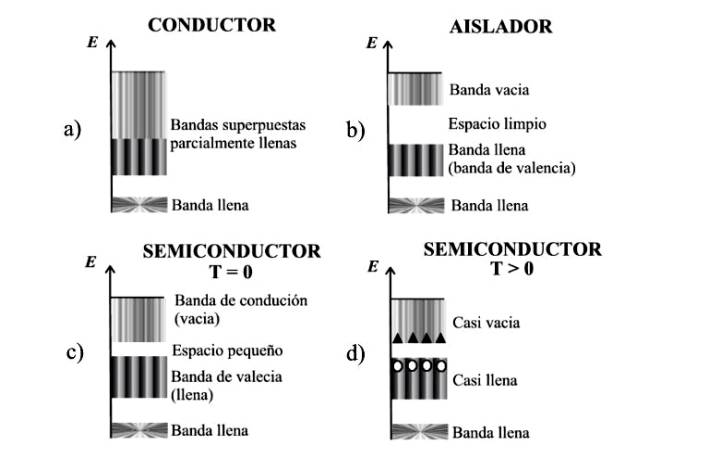
\includegraphics[scale=0.75]{Bandas.jpg} 
					\caption{Diagrama de bandas de energía Aislantes, Conductores y Semiconductores}
				\end{center}
			\end{figure}
			
			\subsection{Aisladores}
			
				En un \textbf{aislador}, el número de electrones dentro del cristal es apenas el suficiente para llenar completamente cierto número de bandas de energía. Entre las bandas llenas y vacías se encuentra una región de energía prohibida tan ancha que es prácticamente imposible, a temperaturas físicamente posibles, excitar térmicamente un número importante de electrones para que atraviesen esta región desde la parte superior de la banda llena más alta a la base de la banda vacía mas baja.
			
			\subsection{Semiconductores}	
			
				Si es muy pequeño el vacío de energía $\Delta \varepsilon$ entre las bandas llenas y vacías, en este tipo de cristal se tiene una probabilidad estadística apreciable de que los electrones puedan excitarse térmicamente de estados cercanos a la parte superior de la banda llena, para atravesar el vacío, hasta los estados cercanos a la base de la banda vacía. Se dispondrá de un número limitado de electrones libres para conducción de corrientes eléctricas en la banda superior casi vacía y, además, los estados electrónicos vacíos que quedan cerca de la parte superior de la banda más baja permiten que esta banda contribuya al flujo de corriente eléctrica a través del mecanismo de conducción por huecos. Un material de esta naturalea se conoce como \textbf{semiconductor}.			
			
			\subsection{Metales}
	
				Si el número de electrones de un cristal no basta para llenar por completo la banda de energía más elevada, sino que la deja sólo llena en parte, muchos de ellos pueden comportarse como electrones libres y servir como carga o portadores de carga. Un cristal de esta índole presentará todas las propiedades características de un \textbf{conductor metálico}: alta conductividad eléctrica y térmica y una gran reflectividad óptica.	
	
	\chapter{Semiconductores I}
		
		\section{Semiconductores uniformes en equilibrio}
		
		Un semiconductor es una substancia cristalina que tiene una estructura de bandas de energía en la que una banda de estados electrónicos, completamente llena a temperatura cero, se separa de otra que está totalmente vacía al cero absoluto por medio de una región angosta de energías prohibidas.\\
		
		En el cero absoluto, el semiconductor es un aislador perfecto, ya que no cuenta con bandas parcialmente llenas. Sin embargo, a temperaturas mas altas, algunos electrones de la banda de valencia pueden adquirir la suficiente \textbf{energía térmica aleatoria} para excitarse a través de la \textbf{banda prohibida} con el fin de convertirse en \textit{electrones} de conducción en la \textbf{banda de conducción} hasta entonces vacía. Los estados vacíos que quedan en la \textbf{banda de valencia} pueden contribuir también a la conductividad comportándose como \textit{huecos} positivamente cargados.\\
		
		En equilibrio, las concentraciones de electrones y huecos siempre deben ser iguales, ya que la excitación térmica de un electrón origina inevitablemente sólo un hueco.\\
		
		\section{Semiconductores intrínsecos}
		
		Un semiconductor en el que los huecos y los electrones se crean exclusivamente mediante una excitación térmica a través de la banda prohibida de energía, se conoce como \textit{semiconductor intrínseco}. Los huecos y los electrones creados de esta manera se denominan \textit{portadores intrínsecos de carga} y la conductividad originada se denomina \textit{conductividad intrínseca}.\\
		
		La población de portadores se describe estadísticamente con la función de distribución de \textit{Fermi-Dirac} y las funciones de densidad de estados para las bandas de valencia y conducción. El comportamiento de los mismos es fundamentalmente el de una partícula libre, con los factores apropiados de masa efectiva. Las funciones de densidad de estados para la banda de conducción y la de valencia son las siguiente:

				\begin{center}
				\boxed{\displaystyle g_c(\varepsilon)=\frac{8\sqrt{2}\pi}{h^3}m_n^{*3/2}\sqrt{\varepsilon-\varepsilon_c} \text{ si } \varepsilon>\varepsilon_c}	\boxed{\displaystyle g_v(\varepsilon)=\frac{8\sqrt{2}\pi}{h^3}m_p^{*3/2}\sqrt{\varepsilon_v-\varepsilon} \text{ si } \varepsilon<\varepsilon_v}
				\end{center}
			
			Donde $m_n^*$ y es la masa efectiva de los electonres de la banda de conducción y $m_p^*$ es la masa efectiva de los huecos de la banda de valencia. La densidad de estados en la región prohibida $\varepsilon_v<\varepsilon<\varepsilon_c$ es cero. Si ambas masas efectivas son iguales, la energía de Fermi debe quedar exactamente en el centro de la región prohibida, de manera tal que la poblaciñón de electrones en la banda de conducción y huecos en la banda de valencia sea la misma.

			\subsection{Estadística de portadores}
			
			En condiciones de equilibrio térmico, el número de electrones $dn_0$ por unidad de volumen que tienen energía en el rango $d\varepsilon$ alrededor de $\varepsilon$ en la banda de conducción de cualquiera semiconductor, intrínseco o con impurezas es:\\
			
			\begin{center}
			$\displaystyle dn_0=f_0(\varepsilon)g_c(\varepsilon)=\frac{8\sqrt{2}\pi}{h^3}m_n^{*3/2}\frac{\sqrt{\varepsilon-\varepsilon_c}d\varepsilon}{1+e^{\frac{\varepsilon-\varepsilon_f}{kT}}}$
			\end{center}
			
			Donde $f_0(\varepsilon)$ representa la función de distribución de Fermi en equilibrio y $g_c(\varepsilon)$ es el factor de densidad de estados.\\
			
			Como $\Delta \varepsilon=\varepsilon_{gap}$, la anchura de la región de energía prohibida, es casi siempre del orden de $1eV$ y $kT\sim\frac{1}{40}eV$ a la temperatura ambiente $300K$, si la energía de Fermi cumple $\varepsilon_c-\varepsilon_f\gg kT$,entonces para todas las energías de la banda de conducción, el factor exponencial es mucho mayor que la unidad, por lo tanto: $\displaystyle f_0(\varepsilon)\cong e^{\frac{-(\varepsilon-\varepsilon_f)}{kT}}$, distribuación con una forma esencialmente maxwelliana.
			
			La aproximación realizada se conoce como \textbf{Aproximación de Boltzmann}. Si se utilizada la misma, se puede integrar y obtener el número total de electrones por unidad de volumen en la banda de conducción.\\
			
			\begin{center}
			$\displaystyle n_0=\int_{\varepsilon_c}^{\infty}dn_0=\frac{8\sqrt{2}\pi}{h^3}m_n^{*3/2}e^{\frac{\varepsilon_f}{kT}}\int_{\varepsilon_c}^{\infty}\sqrt{\varepsilon-\varepsilon_c}e^{-\frac{\varepsilon}{kT}d\varepsilon}=2\left(\frac{2\pi m_n^* kT}{h^2}\right)^{3/2}e^{-\frac{\varepsilon_c-\varepsilon_f}{kT}}=U_ce^{-\frac{\varepsilon_c-\varepsilon_f}{kT}}$\\
			\end{center}
			
			Análogamente para el número de huecos, considerando $dp_0=f_{p0}(\varepsilon)g_v(\varepsilon)d\varepsilon=[1-f_0(\varepsilon)]g_v(\varepsilon)d\varepsilon$\\
			
			Si $\varepsilon_f-\varepsilon_v\gg kT$ el factor exponencial es mucho mayor que la unidad, para todos los valores de $\varepsilon$ en la banda de valencia se puede expresar $\displaystyle f_{p0}(\varepsilon) \cong e^{-\frac{\varepsilon_f-\varepsilon}{kT}}$, que es la aproximación de Boltzmann.Si se utilizada la misma, se puede integrar y obtener el número total de huecos por unidad de volumen en la banda de valencia.\\
			
			\begin{center}
				$\displaystyle p_0=\int_{-\infty}^{\varepsilon_v}dp_0=\frac{8\sqrt{2}\pi}{h^3}m_p^{*3/2}e^{\frac{-\varepsilon_f}{kT}}\int_{-\infty}^{\varepsilon_v}\sqrt{\varepsilon_v-\varepsilon}e^{\frac{\varepsilon}{kT}d\varepsilon}=2\left(\frac{2\pi m_p^* kT}{h^2}\right)^{3/2}e^{-\frac{\varepsilon_f-\varepsilon_v}{kT}}=U_ve^{-\frac{\varepsilon_f-\varepsilon_v}{kT}}$\\
			\end{center}
			
			En una muestra puramente intrínseca se pueden igualar ambos resultados y despejar la energía de Fermi:\\
			
			\begin{center}
				$\displaystyle \varepsilon_f=\frac{\varepsilon_v+\varepsilon_c}{2}+kT \ln\left(\sqrt{\frac{U_v}{U_c}}\right)$
			\end{center}
						
			Reemplazando la expresión de  $U_v$ y $U_c$:\\				
			
			\begin{center}
				\boxed{\displaystyle \varepsilon_{fi}=\frac{\varepsilon_v+\varepsilon_c}{2}+kT \ln\left(\frac{m_p^*}{m_n^*}\right)^{3/4}}
			\end{center}			
			
			Siendo $\varepsilon_{fi}$ la \textbf{energía de Fermi intrínseca}. Si $m_n^*=m_p^*$ entonces el nivel de Fermi se encuentra exactamente en el punto medio de la región prohibida.
			
		\section{Semiconductores extrínsecos}	

			Los \textbf{átomos del grupo V}, llamados \textbf{donadores} tienen cinco electrónes de valencia. Cuatro de ellos se usan para formar enlaces covalentes con átomos circunvecinos del semiconductor y el quinto se enlaza al átomo de impurezas sólo mediante fuerzas electroestáticas que son muy débiles y, por lo tanto, se pueden ionizar con facilidad mediante la agitación térmica de la red a temperaturas ordinarias para proporcionar una \textbf{conducción electrónica adicional}. El átomo de impureza que queda se convierte en un \textbf{ión positivo}. Los cristales que contienen este tipo de impureza existen más electrones que huecos se denominan \textbf{semiconductores tipo n}.\\

			Si se introducen en la red átomos de \textbf{impurezas del grupo III}, llamados \textbf{aceptores}, estos átomos tienen sólo tres electrones de valencia que se usan para formar enlaces covalentes con tres átomos cercanos; pero el cuarto enlace siempre carece de un electrón. En efecto, existe un hueco adicional que se crea en la estructura del enlace covalente en el átomo de la impureza. Este hueco puede emigrar fácilmente alejándose del sitio de la impureza debido a que un electrón adicional del enlace covalente cercano pueda emigrar al sitio de la impureza y llenar el cuarto enlace de par de electrones. Obteniendo \textbf{iones negativos} inmóviles. Los cristales de esta índole se conocen con el nombre de \textbf{semiconductores tipo p}.\\

			La representación estadística de los semiconductores tipo n y p se caracterizan por la presencia del nivel de Fermi superior (para el tipo n) o inferior (para el tipo p) a la posición asociada con el cristal puro o intrínseco.\\

		\section{Ley de acción de masas}	
		
			El producto $n_0 p_0$ es una función exclusiva del ancho de banda prohibida de energía $\Delta \varepsilon$, las masas efectivas y la temperatura, e independiente del nivel de Fermi o del contenido de impurezas.
			
			\begin{center}
				$\displaystyle n_0 p_0=U_c U_v e^{-\frac{\varepsilon_c-\varepsilon_v}{kT}}=U_c U_v e^{-\frac{\Delta \varepsilon}{kT}}$
			\end{center}
	
			Para un semiconductor dado, las masas efectivas y la banda prohibida de energía $\Delta \varepsilon$ son fijas, por lo cuál la expresión anterior solo es función de la temperatura. Esta es una \textbf{ley de acción de masas} que rige las concentraciones relativas de huecos y electrones. Si se está en un estado intrínseco, las concentraciones de huecos y electrones deben ser iguales. $n_0=p_0=n_i(T)$. Dicho producto debe ser el mismo para un semiconductor contaminado con impurezas, debido a que $n_i$ solo depende de la temperatura.	
	
			\begin{center}
					\boxed{n_0 p_0=n_i^2(T)} $\text{ Ley de Acción de Masas}$
			\end{center}		
			
		\section{Contaminación con impurezas}
		
			Existen dos etados cuánticos asociados con cada nivel de impurezas donoras correspondientes a las dos orientaciones del spin permisibles del electrón sobre el átomo donador, tan pronto como se ocupa uno de estos estados, se excluye la ocupación del otro, ya que los requisitos de valencia del ion donador se satisfacen con un solo electrón.\\
			
			En un semiconductor en equilibrio debe haber un hueco térmico o un ión donador positivamente cargado por cada electrón libre, y un electrón térmico o un ión aceptor negativamente cargado por cada hueco libre. Todo el cristal debe ser eléctricamente neutro.
			
			\begin{center}
				$\displaystyle (p_0-n_0)+(N_d-N_a)=0 \Rightarrow U_v e^{-\frac{\varepsilon_f-\varepsilon_v}{kT}}-U_c e^{-\frac{\varepsilon_c-\varepsilon_f}{kT}}+(N_d-N_a)=0$
			\end{center}	
			
			Si se hace la sustitución $\displaystyle \alpha=e^{\frac{\varepsilon_f}{kT}},\beta_c=e^{-\frac{\varepsilon_c}{kT}},\beta_v=e^{\frac{\varepsilon_v}{kT}}$, se llega a la expresión:\\
			
			\begin{center}
				$\displaystyle \alpha^2-\frac{N_d-N_a}{U_c \beta_c}\alpha-\frac{U_v \beta_v}{U_c \beta_c}=0$
			\end{center}
			
			Resolviendo para $\alpha$, tomando el logaritmo del resultado,escogiendo el signo positivo del radical y reemplazando se obtiene:\\
			
			\begin{center}
				$\displaystyle \varepsilon_f=\underbrace{\frac{1}{2}(\varepsilon_v+\varepsilon_c)+kT\ln\left(\frac{m_p^*}{m_n^*}\right)^{\frac{3}{4}}}_{\varepsilon_{fi}}+kT \sinh^{-1}\left(\frac{N_d-N_a}{2\underbrace{\sqrt{U_c U_v}e^{-\frac{\Delta \varepsilon}{2kT}}}_{n_i}}\right)$
			\end{center}
			\begin{center}
				\boxed{\displaystyle \varepsilon_f=\varepsilon_{fi}+kT \sinh^{-1}\left(\frac{N_d-N_a}{2n_i}\right)}
			\end{center}
			
			\begin{figure}[H]
				\begin{center}
					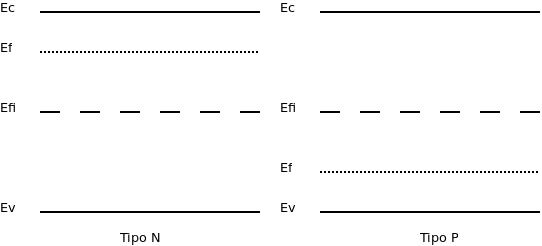
\includegraphics[scale=0.75]{Fermi-dopado.jpeg} 
					\caption{Diagrama de bandas de energía para semiconductores tipo N y tipo P}
				\end{center}
			\end{figure}
			
			\begin{center}
				Semiconductores \textbf{tipo N}: $N_d-N_a>0$ y $\varepsilon_f>\varepsilon_{fi}$\\
				Semiconductores \textbf{tipo P}: $N_d-N_a<0$ y  $\varepsilon_f<\varepsilon_{fi}$\\
			\end{center}
			
			Si la densidad neta de impurezas $|N_d-N_a| \gg n_i$, el número de portadores térmicamente excitados será pequeño en comparación con la cantidad total, entonces $\displaystyle \sinh^{-1}(x) \cong \pm\ln |2x|$ para valores grandes de $x$, finalmente se obtiene:\\
			
			\begin{center}
				\boxed{\displaystyle \varepsilon_f=\varepsilon_{fi} \pm kT \ln \frac{|N_d-N_a|}{n_i}}
			\end{center}
			
			El signo $+$ corresponde para un material tipo n y el signo $-$ para un material tipo p. Los materiales de esta naturaleza se denominan \textbf{fuertemente extrínsecos}.\\
			
			Volviendo a la expresión $p_0-n_0+N_d-N_a=0$ y utilizando la ley de acción de masas $p_0=n_i^2/n_0$ se obtiene:
			
			\begin{center}
				$\displaystyle n_i^2/n_0-n_0+N_d-N_a=0 \Rightarrow n_0^2-(N_d-N_a)n_0-n_i^2=0$\\
			\end{center}
					
			\begin{minipage}[T]{0.4\textwidth}
				\begin{center}
					Si $N_d-N_a>0 \Longrightarrow n_0>p_0 \Longrightarrow \text{ Tipo N }$\\
					$\Downarrow$\\
					Si $N_d-N_a \gg n_i$\\
					$\Downarrow$\\
					$n_0 \cong N_d-N_a$\\
					$\displaystyle p_0 \cong \frac{n_i^2}{N_d-N_a}$\\
				\end{center}
			\end{minipage}
			\begin{minipage}[T]{0.5\textwidth}
				\begin{center}
					Si $N_d-N_a<0 \Longrightarrow p_0>n_0 \Longrightarrow \text{ Tipo P }$\\
					$\Downarrow$\\
					Si $N_a-N_d \gg n_i$\\
					$\Downarrow$\\
					$p_0 \cong N_a-N_d$\\
					$\displaystyle n_0 \cong \frac{n_i^2}{N_a-N_d}$\\
				\end{center}
			\end{minipage}
		
	\chapter{Semiconductores II}	
	
		En un semiconductor se puede alterar la concentración de \textbf{portadores de carga} sin introducir ninguna densidad de carga eléctrica importante. Si tanto huecos como electrones son \textbf{introducidos de a pares}, se puede modificar la concentración volumétrica de portadores sin que se forme ninguna densidad de carga neta	.\\
		
		Los portadores excedentes se pueden crear en los semiconductores iluminando el material con una frecuencia tal que la energía del fotón $\hbar \omega_0$ sea igual o sobrepase la energía de la banda prohibida $\Delta \varepsilon$, liberando electrones libres y dejando los huecos en los sitios de excitación. Los mismos contribuyen a la conductividad del cristal por \textbf{fotoconductividad} y es característico de los semiconductores.
	
		\section{Ecuación de continuidad}
		
			En los semiconductores se generan y recombinan continuamente pares electrón-hueco. En equilibrio térmico, el único proceso de generación es el térmico. La velocidad a la que se generan y recombinan debe ser idéntica. La \textbf{velocidad de recombinación térmica de equilibrio} $g_0[\frac{1}{cm^3seg}]$ es el número de pares electrón-hueco generados por unidad de volumen en unidad de tiempo, mediante la ruptura térmica de enlaces covalentes, independiente de la concentración de electrones y huecos. Este parámetro se relaciona con el tiempo medio que transcurre entre la generación de un electrón o un hueco y su recombinación subsecuente, llamado \textbf{tiempo medio de vida} del portador.\\
			
			\begin{center}
				$\displaystyle g_{0n}=\frac{n_0}{\tau_{n0}}$ y $\displaystyle g_{0p}=\frac{p_0}{\tau_{p0}}$
			\end{center}
			
			Siendo $g_{0n}$ y $g_{0p}$ las velocidades de generación térmica en equilibrio para electrones y huecos, con $\tau_{n0}$ y $\tau_{p0}$ los tiempos de vida promedio respectivamente, en equilibrio.\\
			
			La igualdad de las velocidades de generación y recombinación se aplica a todos los sistemas en estado estacionario, aún los que no están en equilibrio térmico. Lo que implica:\\
			
			\begin{center}
				$g_n=g_p$ y $\displaystyle \frac{n}{\tau_n}=\frac{p}{\tau_p}$
			\end{center}
			
			Con $g_n$ y $g_p$ las velocidades reales de generación, $n$ y $p$ las concentraciones locales y $\tau_n$ y $\tau_p$ el tiempo de vida de electrones y huecos respectivamente.\\
			
			Sean las \textbf{ecuaciones de continuidad}:
			
			\begin{center}
				Para huecos \boxed{\displaystyle -\vec{\nabla}\vec{J}_p+g_p-\frac{p}{\tau_p}=\frac{\partial p}{\partial t}} y para electrones \boxed{\displaystyle -\vec{\nabla}\vec{J}_n+g_n-\frac{n}{\tau_n}=\frac{\partial n}{\partial t}}
			\end{center}	
			
			Para obtener una solución explícita se debe escribir a la \textbf{densidad del flujo de partículas} como la suma de una densidad de flujo de difusión y una densidad de corriente de arrastre producida por cualquier campo eléctrico presente.\\
			
			\begin{center}
				$\displaystyle \vec{J}_p=\underbrace{-D_p\vec{\nabla}p}_{difusion}+\underbrace{p\mu_p\vec{E}}_{arrastre}$ y
				$\displaystyle \vec{J}_n=\underbrace{-D_n\vec{\nabla}n}_{difusion}-\underbrace{n\mu_n\vec{E}}_{arrastre}$
			\end{center}
		
		El término de difusión establece que siempre que existe un gradiente de concentración, se tendrá un flujo neto de corriente de partículas de las regiones de alta concentración a las de baja concentración.\\
		
		Conviene expresar las velocidades de generación como la suma de la velocidad de generación térmica, más la velocidad a la que se generan los portadores en exceso, entonces:
		
		\begin{center}
			$g_n=g_{0n}+g_n^\prime$	 y $g_p=g_{0p}+g_p^\prime$	
		\end{center}
		
		Reemplazando la expresión de la densidad del flujo de partículas en las ecuaciones de continudad se obtiene:\\
		
				\begin{minipage}[t]{0.45\textwidth}
					\begin{center}
						$\displaystyle -\vec{\nabla}(-D_p\vec{\nabla}p+p\mu_p\vec{E})+g_p-\frac{p}{\tau_p}=\frac{\partial p}{\partial t}$\\
						$\Downarrow$\\
						$\displaystyle D_p\vec{\nabla}^2p-\mu_p\vec{\nabla}(p\vec{E})+g_p-\frac{p}{\tau_p}=\frac{\partial p}{\partial t}$\\
						$\Downarrow$\\
						$\displaystyle D_p\vec{\nabla}^2p-\mu_p(\vec{E}\vec{\nabla} p+p\vec{\nabla}\vec{E})+g_p-\frac{p}{\tau_p}=\frac{\partial p}{\partial t}$\\
						$\Downarrow$\\
						$\underbrace{\boxed{\displaystyle D_p\vec{\nabla}^2p-\mu_p(\vec{E}\vec{\nabla} p+p\vec{\nabla}\vec{E})+g_p^\prime-\left(\frac{p}{\tau_p}-\frac{p_0}{\tau_{p0}}\right)=\frac{\partial p}{\partial t}}}_{\text{Ecuación de continuidad para huecos}}$\\
					\end{center}
				\end{minipage}
				\begin{minipage}[t]{0.5\textwidth}
					\begin{center}
						$\displaystyle -\vec{\nabla}(-D_n\vec{\nabla}n-n\mu_n\vec{E})+g_n-\frac{n}{\tau_n}=\frac{\partial n}{\partial t}$\\
						$\Downarrow$\\
						$\displaystyle D_n\vec{\nabla}^2n+\mu_n\vec{\nabla}(n\vec{E})+g_n-\frac{n}{\tau_n}=\frac{\partial n}{\partial t}$\\
						$\Downarrow$\\
						$\displaystyle D_n\vec{\nabla}^2n+\mu_n(\vec{E}\vec{\nabla} n+n\vec{\nabla}\vec{E})+g_n-\frac{n}{\tau_n}=\frac{\partial n}{\partial t}$\\
						$\Downarrow$\\
						$\underbrace{\boxed{\displaystyle D_n\vec{\nabla}^2n+\mu_n(\vec{E}\vec{\nabla} n+n\vec{\nabla}\vec{E})+g_n^\prime-\left(\frac{n}{\tau_n}-\frac{n_0}{\tau_{n0}}\right)=\frac{\partial n}{\partial t}}}_{\text{Ecuación de continuidad para electrones}}$\\
					\end{center}
				\end{minipage}
				
		\section{Ecuación de Einstein}	
		
			Analizando la corriente total de portadores en un semiconductor sin potenciales externos aplicados y teniendo en cuenta que la corriente eléctrica resultante será la carga del portador por el flujo de partículas asociado, se tiene que:\\
			
			\begin{minipage}[t]{0.4\textwidth}
				\begin{center}
					$\displaystyle \vec{I}_p=q\vec{J}_p=-qD_p\vec{\nabla}p+qp\mu_p\vec{E}=0$\\
					$\Downarrow$\\
					$\displaystyle D_p\vec{\nabla}p=p\mu_p\vec{E}$\\
					$\Downarrow$\\
					Considerando $\displaystyle \vec{E}=-\vec{\nabla} \vec{V}$\\
					$\Downarrow$\\
					$\displaystyle dV=\frac{D_p}{\mu_p}\frac{dp}{p}$\\
				\end{center}
			\end{minipage}
			\begin{minipage}[t]{0.4\textwidth}
				\begin{center}
					$\displaystyle \vec{I}_n=q\vec{J}_n=-qD_n\vec{\nabla}n-qn\mu_n\vec{E}=0$\\
					$\Downarrow$\\
					$\displaystyle D_n\vec{\nabla}n=n\mu_n\vec{E}$\\
					$\Downarrow$\\
					Considerando $\displaystyle \vec{E}=-\vec{\nabla} \vec{V}$\\
					$\Downarrow$\\
					$\displaystyle dV=\frac{D_n}{\mu_n}\frac{dn}{n}$\\
				\end{center}
			\end{minipage}
			\\
			\\
			\begin{center}
				Combinando ambas expresiones se tiene la \textbf{Relación de Einstein}:\\
				\boxed{\displaystyle \frac{D_p}{\mu_p}=\frac{D_n}{\mu_n}}
			\end{center}
		
		\section{Impurificación homogénea}
	
			Se aproximará utilizando la \textbf{condición de neutralidad eléctrica} o suposición de balance de carga. Se supondrá que la densidad de electrones en exceso $\delta n=n-n_0$ se equilibra mediante una densidad de huecos en exceso $\delta p=p-p_0$, inicialmente se considerará:\\
		
			\begin{center}
				 $\delta n=n-n_0=p-p_0=\delta p$
			\end{center}
		
			Considerando muestras homogéneamente contaminadas, $n_0$ y $p_0$ son constantes y los gradientes y las derivadas del tiempo para $n$ y $p$ son iguales a los gradientes y a las derivadas del tiempo de $\delta n$ y $\delta p$. Por lo tanto se puede escribir:\\
			
			Teniendo $g_n^\prime=g_p^\prime=g^\prime$\\
	
			Para huecos: $\displaystyle D_p\vec{\nabla}^2(\delta p)-\mu_p(\vec{E}\vec{\nabla} (\delta p)+p\vec{\nabla}\vec{E})+g^\prime-\left(\frac{p_0+\delta p}{\tau_p}-\frac{p_0}{\tau_{p0}}\right)=\frac{\partial (\delta p)}{\partial t}$\\

			Para electrones: $\displaystyle D_n\vec{\nabla}^2(\delta p)+\mu_n(\vec{E}\vec{\nabla}(\delta p)+n\vec{\nabla}\vec{E})+g^\prime-\left(\frac{p_0+\delta p}{\tau_p}-\frac{p_0}{\tau_{p0}}\right)=\frac{\partial (\delta p)}{\partial t}$\\
		
			Multiplicando la primer ecuación por $p\mu_p$, la segunda ecuación por $n\mu_n$ y sumando ambas se obtiene:\\
		
			\begin{center}
				$\displaystyle \frac{n\mu_n D_p+p\mu_p D_n}{n\mu_n+p\mu_p}\vec{\nabla}^2(\delta p)-\frac{\mu_n \mu_p (n_0-p_0)}{n\mu_n-p\mu_p}\vec{E}\vec{\nabla} (\delta p)+g^\prime -\left(\frac{p_0+\delta p}{\tau_p}-\frac{p_0}{\tau_{p0}}\right)=\frac{\partial (\delta p)}{\partial t}$
			\end{center}
			\begin{center}	
				$\Downarrow$
			\end{center}
			\begin{center}
				Definiendo $\displaystyle D^*=\frac{(n+p)D_nD_p}{nD_n+pD_p}$ y $\displaystyle \mu^*=\frac{(n_0-p_0)\mu_n\mu_p}{n\mu_n+p\mu_p}$\\
			\end{center}
			\begin{center}	
				$\Downarrow$
			\end{center}
			\begin{center}
				$\underbrace{\displaystyle D^*\vec{\nabla}^2(\delta p)-\mu^*\vec{E}\vec{\nabla} (\delta p)+g^\prime -\frac{\delta p}{\tau}=\frac{\partial (\delta p)}{\partial t}}_{\text{Ecuación de transporte ambipolar}}$
			\end{center}	
			\begin{center}
			Donde $\tau$ es el \textbf{tiempo de vida del portador en exceso} definido por:
			\end{center}
			\begin{center}
				 $\displaystyle \frac{\delta p}{\tau}=\frac{p_0+\delta p}{\tau_p}-\frac{p_0}{\tau_{p0}}=\frac{n_0+\delta p}{\tau_n}-\frac{n_0}{\tau_{n0}}$
			\end{center}
	
			Para facilitar el problema, se restringirá el análisis al \textbf{caso de nivel bajo}, donde los parámetros de la ecuación de transporte ambipolar son substancialmente constantes y permiten obtener soluciones analíticas.\\
			
			\begin{itemize}
			\item Si el material es \textbf{fuertemente extrínseco tipo N} ($n_0 \gg p_0,\delta p$), los parámetros de la ecuación de transporte ambipolar se reducen a: $\tau=\tau_p=\tau_{p0}$, $D^*=D_p$, $\mu^*=\mu_p$ y entonces:\\
			
				\begin{center}
					\boxed{\displaystyle D_p\vec{\nabla}^2(\delta p)-\mu_p\vec{E}\vec{\nabla} (\delta p)+g^\prime -\frac{\delta p}{\tau_{p0}}=\frac{\partial (\delta p)}{\partial t}}
			\end{center}	
			\item Si el material es \textbf{fuertemente extrínseco tipo P} ($p_0 \gg n_0,\delta n$), los parámetros de la ecuación de transporte ambipolar se reducen a: $\tau=\tau_n=\tau_{n0}$, $D^*=D_n$, $\mu^*=\mu_n$ y entonces:\\
			
				\begin{center}
				\boxed{\displaystyle D_n\vec{\nabla}^2(\delta n)-\mu_n\vec{E}\vec{\nabla} (\delta n)+g^\prime -\frac{\delta n}{\tau_{n0}}=\frac{\partial (\delta n)}{\partial t}}
			\end{center}
	\end{itemize}
	
	
			\subsection{Casos particulares de la ecuación de continuidad}
		
				\subsubsection{Campo aplicado nulo, sin generación de portadores, dopado espacial uniforme}	
				
					\begin{center}
						$\displaystyle D_n\underbrace{\vec{\nabla}^2(\delta n)}_{\text{0,uniforme}}-\mu_n\underbrace{\vec{E}}_{\text{0}}\underbrace{\vec{\nabla} (\delta n)}_{\text{0,uniforme}}+\underbrace{g^\prime}_{\text{0, sin generación}} -\frac{\delta n}{\tau_{n0}}=\frac{\partial (\delta n)}{\partial t}$
					\end{center}
					\begin{center}
						$\Downarrow$
					\end{center}
					\begin{center}
						$\displaystyle  -\frac{\delta n}{\tau_{n0}}=\frac{\partial (\delta n)}{\partial t}$
					\end{center}
					\begin{center}
						$\Downarrow$
					\end{center}
					\begin{center}
						$\displaystyle \delta n=n-n_0=\delta n(t=0)e^{-\frac{t}{\tau}}=\delta p$
					\end{center}
	
					La densidad de portadores en exceso se pierde en todos los puntos de un modo exponencial en función de una constante de tiempo $\tau$ igual al tiempo de vida medio de los portadores en exceso.\\
	
				\subsubsection{Estado estacionario, unidimensional, sin campo aplicado y sin generación de portadores}
	
					\begin{center}
						$\displaystyle D_n\vec{\nabla}^2(\delta n)-\mu_n\underbrace{\vec{E}}_{\text{0}}\vec{\nabla} (\delta n)+\underbrace{g^\prime}_{\text{0, sin generación}} -\frac{\delta n}{\tau_{n0}}=\underbrace{\frac{\partial (\delta n)}{\partial t}}_{\text{0,estacionario}}$
					\end{center}
					\begin{center}
						$\Downarrow$
					\end{center}
					\begin{center}
						$\displaystyle D_n \tau_{n0}\frac{d^2 (\delta n)}{d x^2}=\delta n \Rightarrow L_n^2\frac{d^2 (\delta n)}{d x^2}=\delta n$
					\end{center}
					\begin{center}
						$\Downarrow$
					\end{center}
					\begin{center}
						$\displaystyle \delta n=n(x)-n_0=A e^{\frac{x}{L_n}}+B e^{-\frac{x}{L_n}}$
					\end{center}
	
					Que presenta una singularidad en $x=0$, donde se estableció la fuente plana de portadores, entonces:\\
					
					\begin{minipage}[t]{0.45\textwidth}
						\begin{center}
							$x>0$\\
							$\Downarrow$\\
							$\displaystyle \delta n_+(x)=n_+(x)-n_0=A_+ e^{\frac{x}{L_n}}+B_+ e^{-\frac{x}{L_n}}$\\
							$\Downarrow$\\
							Existe velocidad de recombinación volumétrica diferente de cero, entonces $A_+=B_-=0$\\
							$\Downarrow$\\
							$\displaystyle \delta n_+(x)=n_+(x)-n_0=A_0 e^{-\frac{x}{L_n}}$\\
						\end{center}
					\end{minipage}
					\begin{minipage}[t]{0.45\textwidth}
						\begin{center}
							$x<0$\\
							$\Downarrow$\\
							$\displaystyle \delta n_-(x)=n_-(x)-n_0=A_- e^{\frac{x}{L_n}}+B_- e^{-\frac{x}{L_n}}$\\
							$\Downarrow$\\
							Existe velocidad de recombinación volumétrica diferente de cero, entonces $A_+=B_-=0$\\
							$\Downarrow$\\
							$\displaystyle \delta n_+(x)=n_+(x)-n_0=A_0 e^{\frac{x}{L_n}}$\\
						\end{center}
					\end{minipage}
	
					\begin{center}
						$\Downarrow$\\
						$\displaystyle \delta n(x)=\delta n(x=0)e^{-\frac{x}{L_n}}=\delta p(x)$
					\end{center}
	
				\subsubsection{Estado estacionario,unidimensional, sin generación de portadores, campo constante aplicado}
	
				\begin{center}
						$\displaystyle D_n\vec{\nabla}^2(\delta n)-\mu_n\underbrace{\vec{E}}_{E_0}\vec{\nabla} (\delta n)+\underbrace{g^\prime}_{\text{0, sin generación}} -\frac{\delta n}{\tau_{n0}}=\underbrace{\frac{\partial (\delta n)}{\partial t}}_{\text{0,estacionario}}$
					\end{center}
					\begin{center}
						$\Downarrow$
					\end{center}
					\begin{center}
						$\displaystyle \frac{d^2 (\delta n)}{d x^2}-\frac{\mu_n E_0}{D_n}\frac{d (\delta n)}{dx}-\frac{\delta n}{L_n}=0 \Rightarrow \gamma_n=\frac{\mu_n E_0}{2 D_n} \pm \sqrt{\frac{\mu_n E_0}{2D_n}^2+\frac{1}{L_n}}$				
					\end{center}		
					\begin{center}
						$\Downarrow$
					\end{center}			
					\begin{center}
						$\displaystyle \delta n(x)=n(x)-n_0=A e^{\gamma_n^+ x}+B e^{\gamma_n^- x}$
					\end{center}
					\begin{center}
						$\Downarrow$
					\end{center}			
					\begin{center}
						$\displaystyle \delta n(x) =n(x)-n_0=A_0 e^{x}(e^{\gamma_n^+}\cdot \{x>0\}+e^{\gamma_n^-}\cdot \{x<0\})=\delta p(x)$
					\end{center}
	
	Si el campo $\vec{E}$ está presente en la dirección en que $x$ crece, entonces el transporte de los portadores en exceso será hacia la derecha, favorecido por la acción del campo, en tanto que se retrasa el transporte de portadores en dirección opuesta. El flujo de partículas resultante será el producto tanto de la difusión por tener un gradiente de concentración, como del arrastre debido al campo eléctrico.
	
	\chapter{Junturas}
		\section{Juntura PN}
		
			Se denomina juntura PN a la \textbf{región angosta de transición} que separa una región extrínseca tipo N de una región extrínseca tipo P.\\
		
			La transición puede ser abrupta, donde cada región contiene una concentración neta más o menos constante de impurezas donoras o aceptoras; o graduada, donde $N_d$ y $N_a$ son funciones de la distancia a la unión en dirección de la normal, partiéndo con $N_d>N_a$ en el lado tipo N, ambas cantidades se igualan en la unión y se llega al lado tipo P con $N_a>N_d$.\\
		
			Para la mayoría de dispositivos más importantes, la representación mas aceptable es la \textbf{aproximación de la unión abrupta}.\\
		
				\begin{figure}[H]
					\begin{center}
						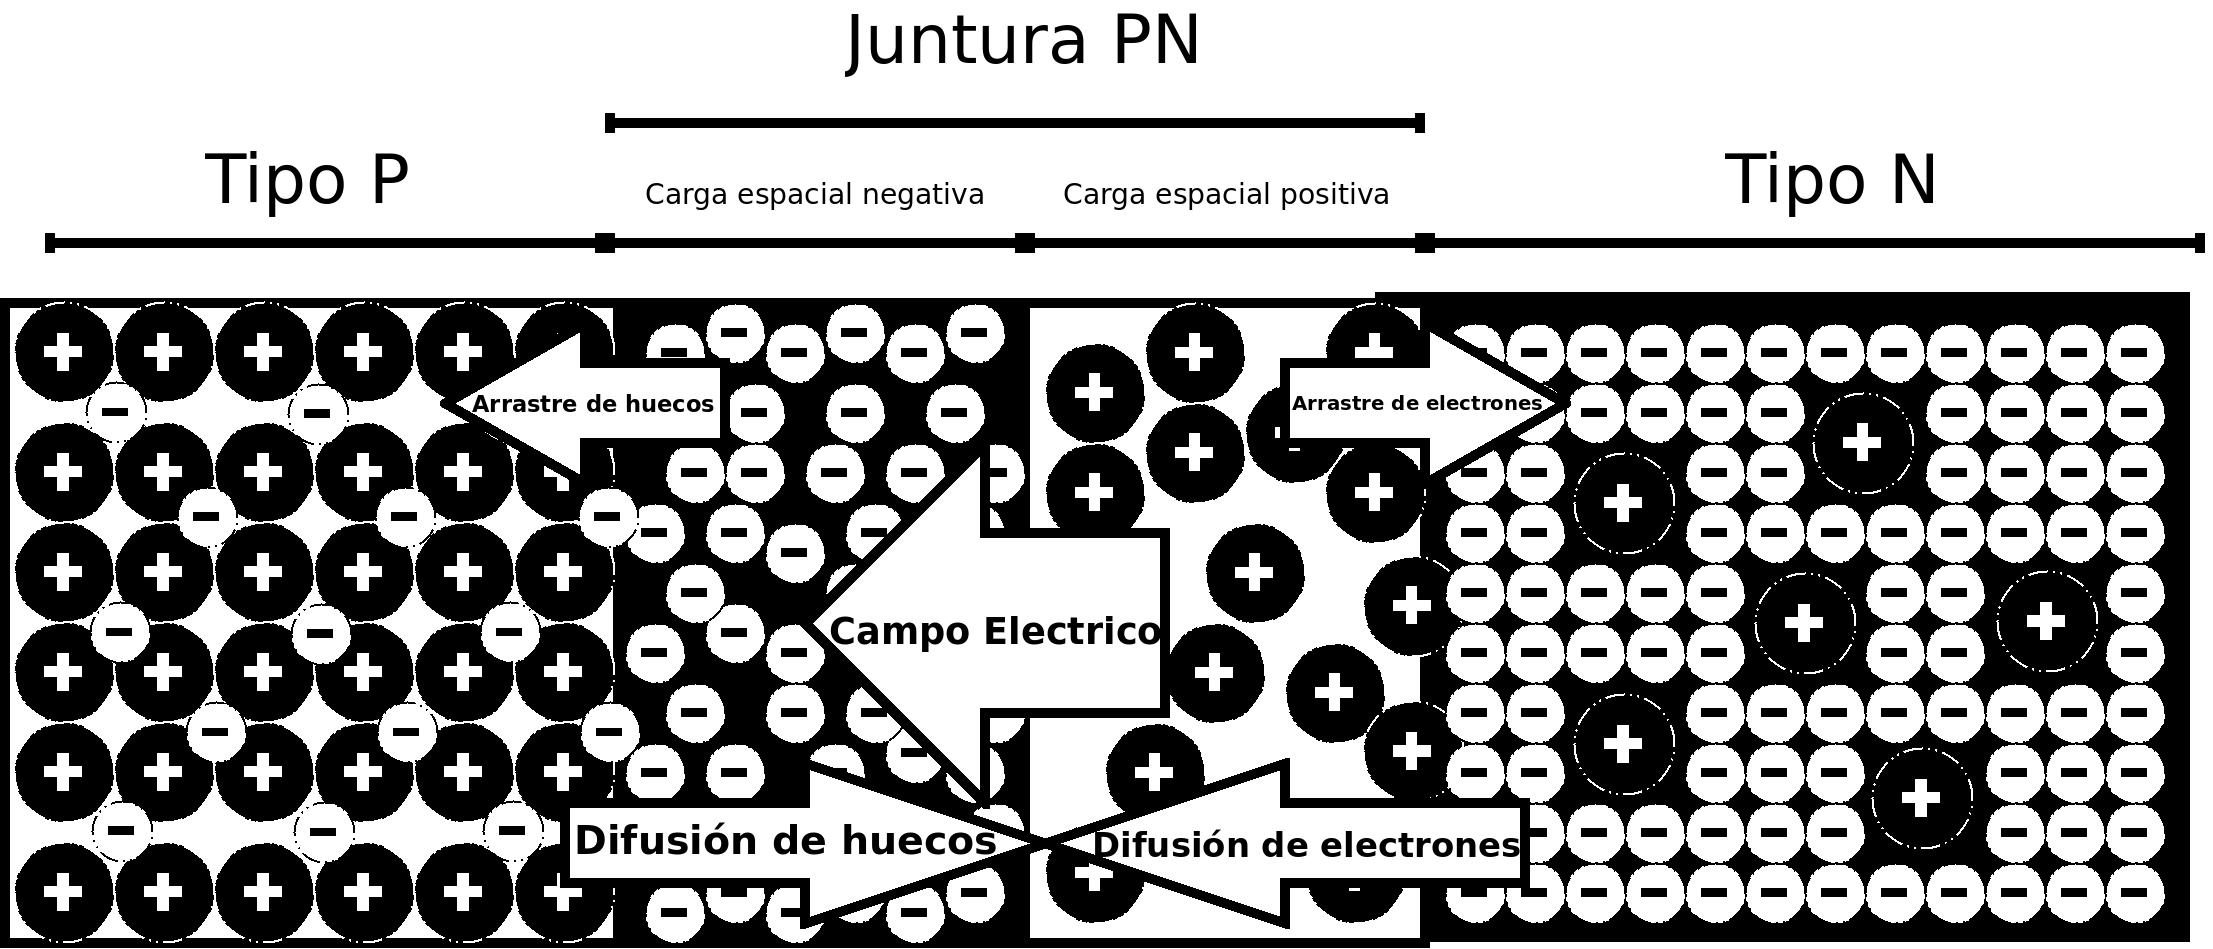
\includegraphics[scale=0.2]{Juntura-PN.jpeg}
						\caption{Juntura-PN}
					\end{center}
				\end{figure}			
		
			\begin{minipage}[t]{0.2\textwidth}
				\begin{center}
					Región Tipo P
					\begin{itemize}
						\item $n_{p0}=\frac{n_i^2}{N_a}$
						\item $p_{p0}=N_a$
					\end{itemize}
				\end{center}
			\end{minipage}
			\begin{minipage}[t]{0.2\textwidth}
				\begin{center}
					Región negativa
					\begin{itemize}
						\item $n_i>n>\frac{n_i^2}{N_a}$
						\item $N_a>p>n_i$
					\end{itemize}
				\end{center}
			\end{minipage}
			\begin{minipage}[t]{0.2\textwidth}
				\begin{center}
					Región positiva
					\begin{itemize}
						\item $N_d>n>n_i$
						\item $n_i>p>\frac{n_i^2}{N_d}$
					\end{itemize}
				\end{center}
			\end{minipage}
			\begin{minipage}[t]{0.2\textwidth}
				\begin{center}
					Región Tipo N
					\begin{itemize}
						\item $n_{n0}=N_d$
						\item $p_{n0}=\frac{n_i^2}{N_d}$
					\end{itemize}
				\end{center}
			\end{minipage}					
		\vfill
		En el instante de formación de la juntura PN, existe una concentración uniforme $n_{n0}$ de electrones libres móviles y $p_{n0}$ de huecos libres móviles en el lado N, extendiéndose hasta la juntura, y en el lado P, una concentración uniforme $p_{p0}$ de huecos móviles y $n_{p0}$ de electrones libres que se extienden también hasta la juntura. Relacionadas con las densidades netas de donores ($N_d$) y aceptores ($N_a$), en tanto que en ambos lados las densidades de electrones y huecos satisfacen la relación:
		
				 \begin{center}
					 $\displaystyle n_{n0}p_{n0}=p_{p0}n_{p0}=n_i^2$
				 \end{center}
			
			\subsection{Equilibrio}
			
				\begin{itemize}
					\item \textbf{Difusión de huecos:} Puesto que la concentración $p_{p0}$ de huecos del lado P es mucho mayor que la concentración de huecos $p_{n0}$ del lado N, existe un gradiente enorme en la concentración de huecos entre ambas regiones. Generando una corriente de difusión que hace que los huecos de la región P fluyan descendiendo por el gradiente de concentración hacia la región N. Dejando a la región P cercana a la juntura vacía de portadores mayoritarios.
					\item \textbf{Difusión de electrones:} Puesto que la concentración $n_{n0}$ de electrones del lado N es mucho mayor que la concentración de electrones $n_{p0}$ del lado P, existe un gradiente enorme en la concentración de electrones entre ambas regiones.Generando una corriente de difusión que hace que los electrones de la región N fluyan descendiendo por el gradiente de concentración hacia la región P. Dejando a la región N cercana a la juntura vacía de portadores mayoritarios.
				\end{itemize}	
				
					Sin embargo, este flujo de difusión inicial no puede continuar indefinidamente, debido a que en las regiones cercanas a la juntura hay deficiencia de portadores mayoritarios, las cargas de los iones fijos donores y aceptores cercanos de la juntura ya no están balanceadas por las cargas de los portadores libres móviles que estaban allí inicialmente. Por lo tanto se establece un campo eléctrico que se opone al flujo de los electrones que salen de la región N y al flujo de los huecos que salen de la región P. 	
				
				\begin{itemize}
					\item \textbf{Arrastre de huecos:} Debido al campo eléctrico generado por los iones fijos en la zona de vaciamiento, los huecos se ven afectados por una fuerza coulombiana que los moviliza desde el lado N al lado P.
					\item \textbf{Arrastre de electrones:} Debido al campo eléctrico generado por los iones fijos en la zona de vaciamiento, los electrones se ven afectados por una fuerza coulombiana que los moviliza desde el lado P al lado N.
				\end{itemize}			
			
				La magnitud del campo se desarrolla hasta el punto en que su efecto contrarresta exactamente la tendencia de los portadores mayoritarios a difundirse	. Se establece una condición de equilibrio dinámico en la que la región cercana a la juntura queda vacía de portadores mayoritarios y en la que forman fuertes capas de carga espacial que contiene campos eléctricos altos cerca de la juntura.				
			
			\subsection{Potencial de contacto}
			
				Mas allá de las regiones de la carga espacial no existe una densidad de carga y, por tanto, el potencial electroestático es constante. Puesto que el estado del sistema es de equilibrio térmico, la energía de Fermi $\varepsilon_f$ debe ser la misma en todo el sistema, permitiendo describir las bandas de energía abrupta. Existe un potencial de contacto interno $e\phi_0$ desarrollado entre las dos regiones.
				
				\begin{figure}[H]
					\begin{center}
						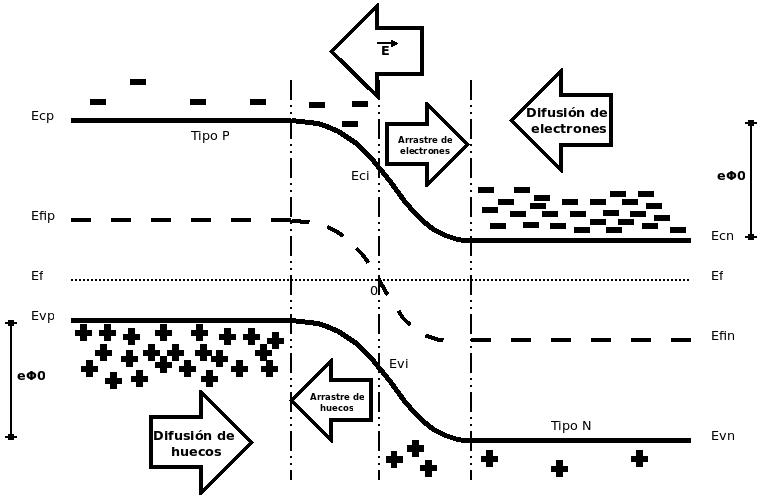
\includegraphics[scale=0.5]{Fermi-PN.jpeg}
						\caption{Diagrama de bandas de energía cerca de la unión PN en ausencia de tensión aplicada}
					\end{center}
				\end{figure}			
						
				
				El valor del potencial de contacto interno $\phi_0$ se determina fácilmente a partir de los valores de la densidad de electrones (o huecos) en equilibrio a ambos lados de la juntura, lejos de las regiones de carga espacial.
				
				\begin{center}
					Para la densidad de electrones del lado N: $\displaystyle n_{n0}=U_c e^{-\frac{\varepsilon_{cn}-\varepsilon_f}{kT}}$\\
					Para la densidad de electrones del lado P: $\displaystyle n_{p0}=U_c e^{-\frac{\varepsilon_{cp}-\varepsilon_f}{kT}}$\\		
				\end{center}				
			
			Despejando $\varepsilon_{cn}$ y $\varepsilon_{cp}$, considerando que todos los donores y aceptores de las regiones N y P están ionizados y si las dos regiones P y N son fuertemente extrínsecas, se puede obtener la energía potencial interna:\\
			
			\begin{center}
				$e\phi_0=\varepsilon_{cp}-\varepsilon_{cn}=kT\ln \frac{n_{n0}}{n_{p0}} \Rightarrow \phi_0=\frac{kT}{e}\ln \frac{n_{n0}p_{p0}}{n_i^2} \Rightarrow$ \boxed{\displaystyle \phi_0=\frac{kT}{e}\ln \frac{N_dN_a}{n_i^2}}
			\end{center}			
			
			Limitado a situaciones en que las estadísticas de Boltzmann se pueden utilizar para describir la distribución de portadores en equilibrio.
			
			\subsection{Fuera del equilibrio}
			
				Aplicando una tensión externa a la juntura PN, puesto que las regiones de carga espacial a ambos lados de la juntura tienen una deficiencia de portadores, estas regiones poseen una resistividad mucho mayor que cualquier otra parte del cristal, por lo tanto casi toda la caída de potencial se producirá en estas regiones.\\
				
				Si la juntura PN se usa como rectificador, se obtiene una condición de \textbf{baja impedancia} cuando la región N se conecta a la terminal negativa y la región P a la positiva de la fuente externa de tensión. Esta polaridad se conoce como estado de \textbf{polarización directa}. Se considera que el signo del potencial externamente aplicado como positivo. El efecto es \textbf{reducir la altura de la barrera de potencial}. Si la caída de potencial en las regiones volumétricas N y P que quedan fuera de la capa de carga espacial es despreciable en comparación con la producida en la juntura, la altura de la barrera será de $e(\phi_0-V_0)$, siendo $V_0$ el potencial externo aplicado.\\
			
				\begin{figure}[H]
					\begin{center}
						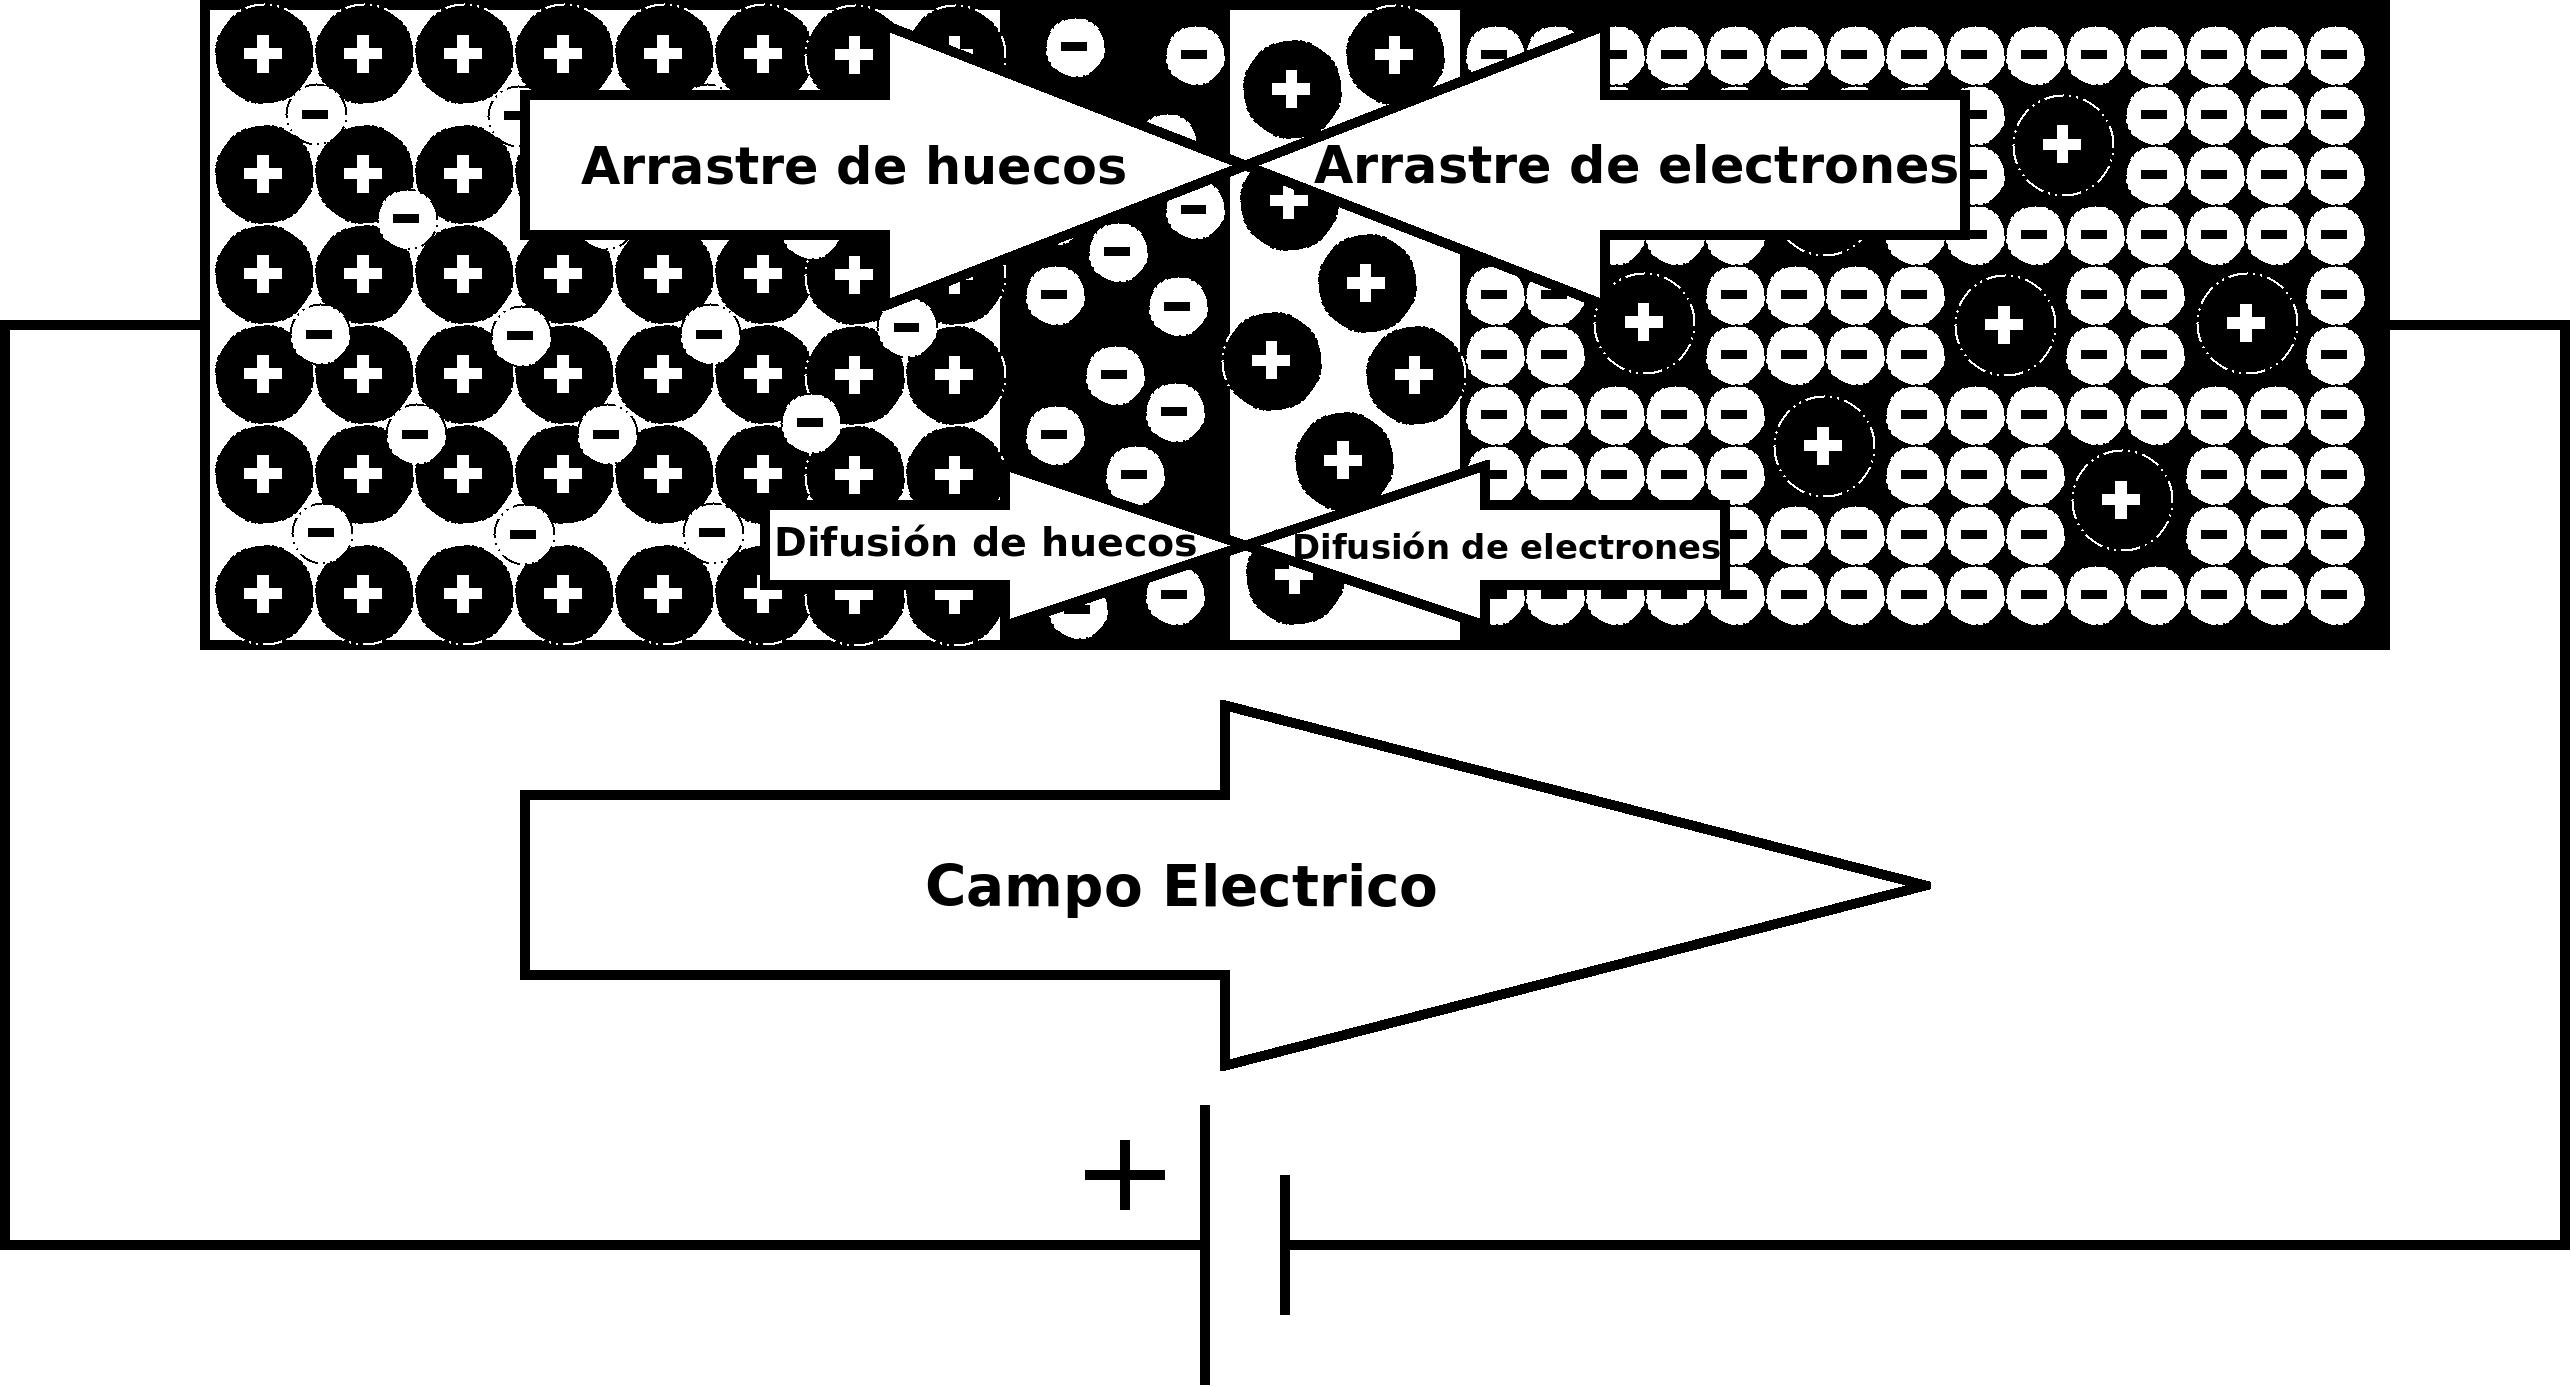
\includegraphics[scale=0.15]{Juntura-PN-dir.jpeg}
						\caption{Juntura-PN en polarización directa}
					\end{center}
				\end{figure}					
			
				Si se invierte la polaridad de la fuente de potencial externo (considerando al signo negativo), se observa que \textbf{la altura de la barrera de potencial se incrementa}.Si la caída de potencial en las regiones volumétricas N y P que quedan fuera de la capa de carga espacial es despreciable en comparación con la producida en la juntura, la altura de la barrera será de $e(\phi_0-V_0)$, siendo $V_0$ negativo. Esta estructura presenta una \textbf{impedancia muy alta} y se dice que la tensión aplicada es una \textbf{polarización inversa}.\\
			
				\begin{figure}[H]
					\begin{center}
						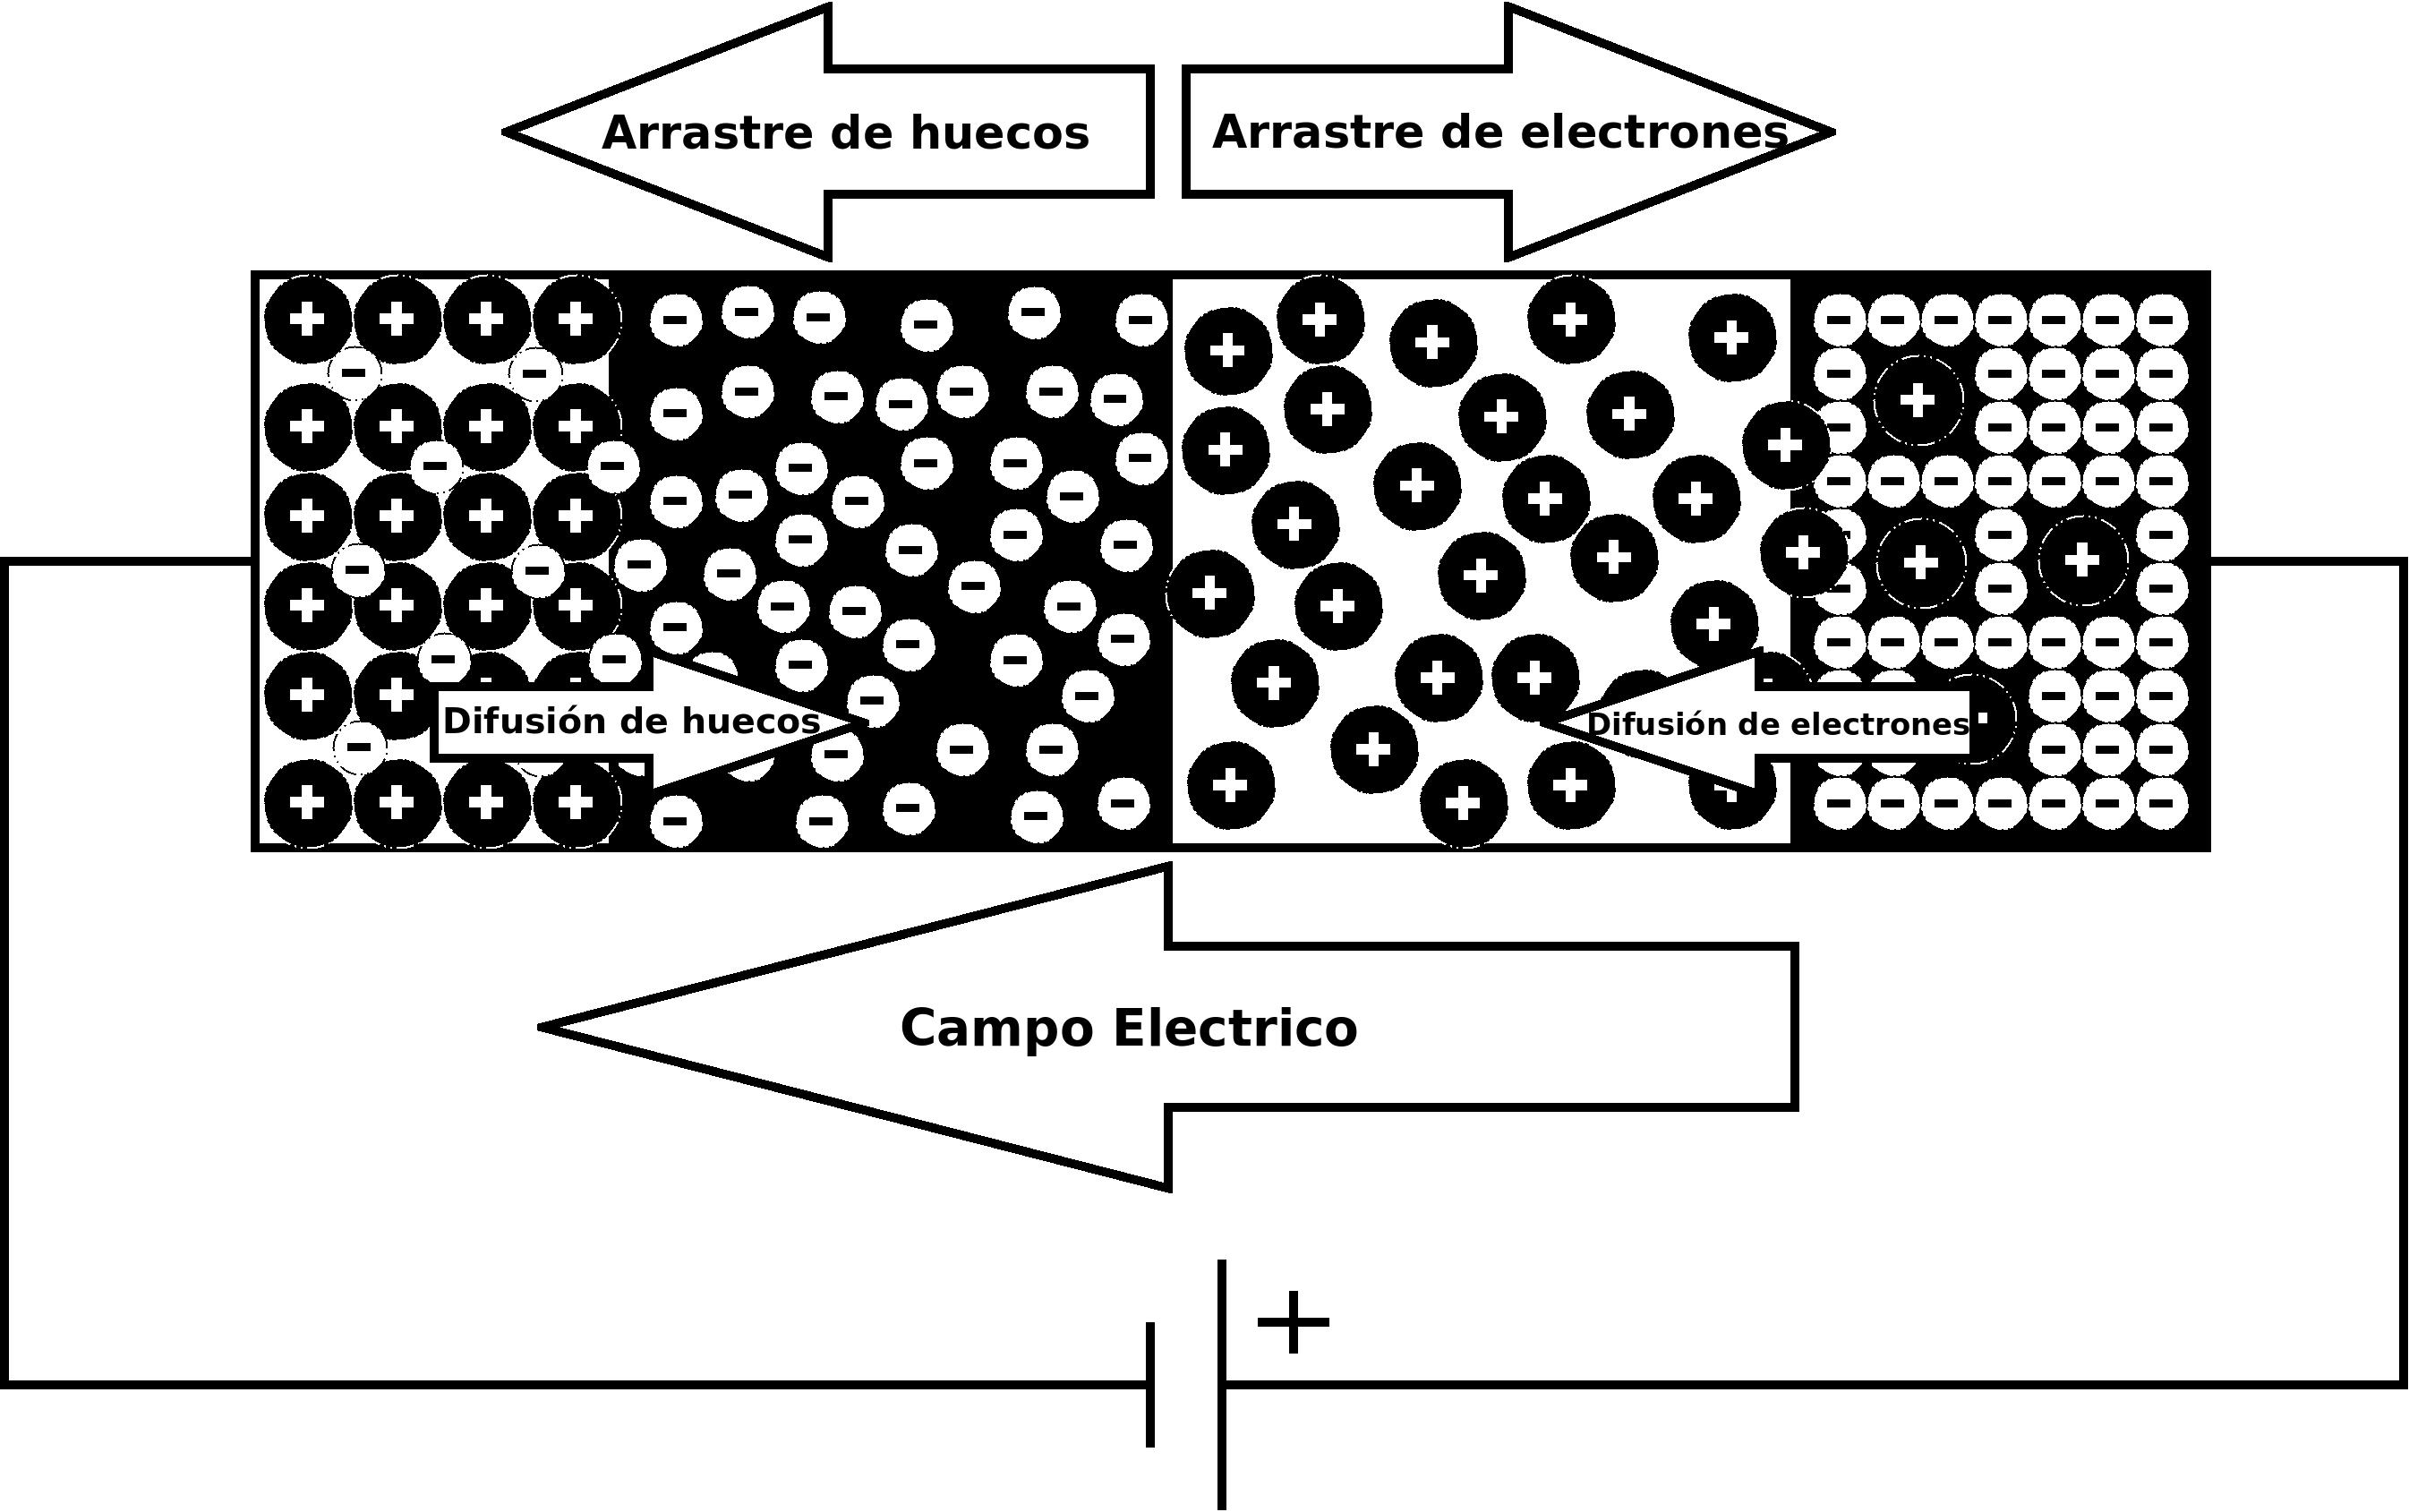
\includegraphics[scale=0.15]{Juntura-PN-inv.jpeg}
						\caption{Juntura-PN en polarización inversa}
					\end{center}
				\end{figure}					
			
			Si se aplica un potencial inverso mas elevado, el polo positivo de la fuente atraerá los electrones del lado N, y los transportará al lado P, donde llegan con una energía cinéctica elevada. Suponiendo que ya no existen huecos con los cuales recombinarse, debido a una saturación del material, ya que la zona de vaciamiento es excesivamente grande, los electrones tendrán la suficiente energía como para atravesar la barrera de potencial, alcanzando nuevamente el lado N, pero esta vez pudiendo colisionar con los átomos de la red y destruyendo los enlaces covalentes, liberando mas electrones que repetirán el mismo ciclo. A este efecto se le denomina \textbf{efecto avalancha} y ocurre a partir de la \textbf{tensión de ruptura}, para la cual el dispositivo deja de actuar como un circuito abierto.			
			
			
			Será mas sencillo visualizar el efecto del potencial externo en un diagrama de bandas de energía:\\
			
			\begin{figure}[H]
					\begin{center}
						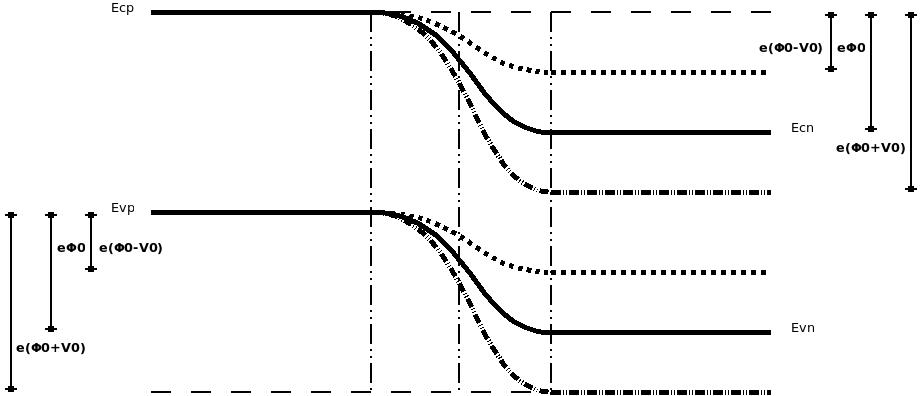
\includegraphics[scale=0.5]{Fermi-PN-dir-inv.jpeg}
						\caption{Diagrama de la energía potencial ante tensión externa aplicada}
					\end{center}
				\end{figure}		
			
			\subsection{Ecuación y distribución de corrientes}
		
				En el \textbf{estado de equilibrio} habrá cierto número de electrones presentes como portadores mayoritarios el en lado N, que tienen la suficiente energía para saltar la barrera de potencial y difundirse en el lado P de la juntura. En la región P, estos electrones constituyen portadores minoritarios y pueden, después de cierto tiempo, desaparecer mediante su recombinación con huecos. Se tiene por lo tanto, una correinte de electrones de la región N pasando por la untura, hasta la región P, donde se pierden por recombinación.Este flujo electrónico de equilibrio se citará como \textbf{flujo de recombinación} $\vec{J}_{nr}$\\
				
				En la condición de equilibrio no puede haber un flujo neto de corriente, cualquier proceso microscópico de transporte y su inversa deben proceder a la misma velocidad. La inversa de este proceso es la generación de pares electrón-hueco en el lado P de la juntura, y la difusión subsecuente de electrones a través de la juntura hacia el lado N, en donde se convierten en portadores mayoritarios. Este proceso inverso conduce a una corriente electrónica que fluye de la región P a la región N y que se denomina \textbf{flujo de generación} $\vec{J}_{ng}$. En equilibrio, el flujo de partículas resultante es $\vec{J}_{ng}=-\vec{J}_{nr}$.\\
				
				Análogamente a los huecos, existe un \textbf{flujo de recombinación} $\vec{J}_{pr}$ que se origina cuando los huecos de la región P se desplazan sobre la barrera hasta la región N, en donde se recombinan con los electrones. Acompañado por un \textbf{flujo de generacion} $\vec{J}_{pg}$ que se crea mediante la generación térmica de pares en la región N, seguida de la difusión de huecos térmicamente generados a través de la juntura. En equilibrio, el flujo de partículas resultante es $\vec{J}_{pg}=-\vec{J}_{pr}$.\\
				
				En estado de equilibrio, los flujos totales de huecos y electrones a través de la juntura son iguales a cero.\\
				
				En \textbf{polarización inversa}, la altura de la barrera de potencial en la juntura aumenta en una cantidad igual a $-eV_0$, con $V_0$ la tensión aplicada. En esas condiciones es difćil para los portadores vencer la barrera por difusión y, por lo tanto, \textbf{$\vec{J}_{nr}$ y $\vec{J}_{pr}$ se hacen muy pequeños}. Sin embargo, $\vec{J}_{ng}$ y $\vec{J}_{pg}$ depeden sólo de la velocidad de generación térmica de pares electrón-hueco en las regiones volumétricas respectivas y no se ven reducidos. Conforme se incremente la tensión de polarización, la densidad de corriente a través de la juntura tiende a un valor pequeño constante $-e(\vec{J}_{pg}-\vec{J}_{ng})$ denominado \textbf{corriente de saturación}, limitada por el número de pares térmicamente generados, depende sólo de parámetros del material y la temperatura.\\
				
				\begin{figure}[H]
					\begin{center}
						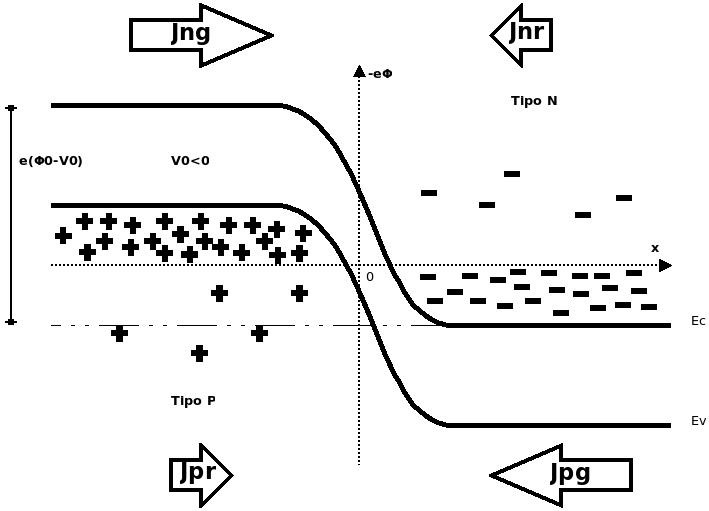
\includegraphics[scale=0.5]{Juntura-inv.jpeg}
						\caption{Diagrama de la energía potencial en polarización inversa}
					\end{center}
				\end{figure}						
				
				
				Cuando se aplica una tensión de \textbf{polarización directa}, la altura de la barrera de potencial se reduce y es muy fácil para los electrones mayoritarios del lado N y los huecos mayoritarios del lado P, difundirse sobre la barrera hacia los lados opuestos respectivos en donde pueden convertirse en portadores minoritarios y, finalmente, recombinarse. \textbf{Tanto $\vec{J}_{pr}$ como $\vec{J}_{nr}$ pueden hacerse muy grandes} en comparación a sus valores de equilibrio. No obstante, las corrientes de generación $\vec{J}_{ng}$ y $\vec{J}_{pg}$ permanecen iguales, ya que están limitadas por la velocidad de generación térmica.\\
				
				\begin{figure}[H]
					\begin{center}
						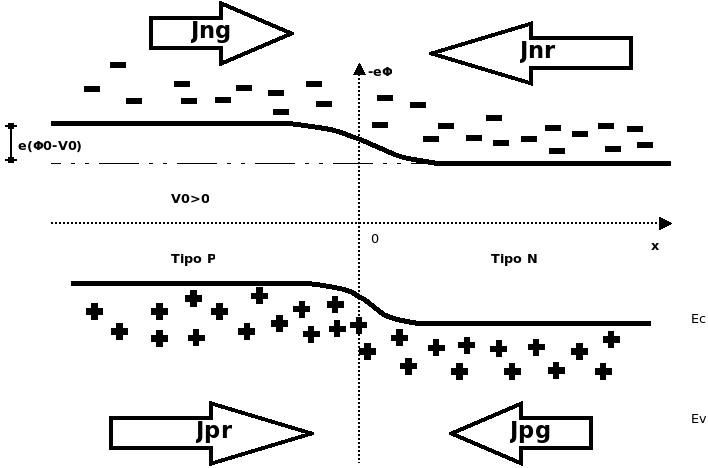
\includegraphics[scale=0.5]{Juntura-dir.jpeg}
						\caption{Diagrama de la energía potencial en polarización directa}
					\end{center}
				\end{figure}				
				
				La estructura de la juntura presenta una impedancia elevada en la dirección de polarización inversa y una impedancia muy pequeña en la dirección de polarización directa, por lo que se comporta como un \textbf{diodo}.\\
				
				\begin{figure}[H]
					\begin{center}
						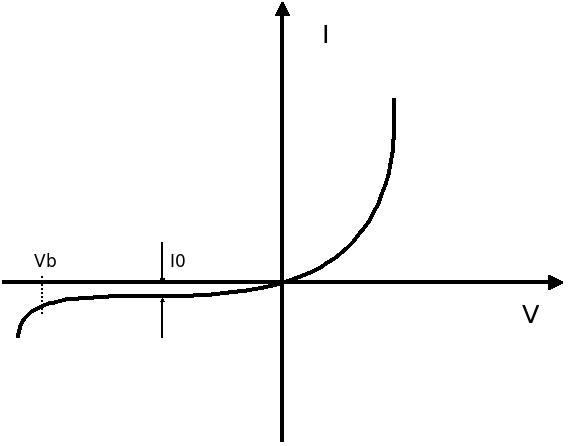
\includegraphics[scale=0.5]{Diodo-PN.jpeg}
						\caption{Relación corriente-tensión en la juntura PN en la región de ruptura inversa}
					\end{center}
				\end{figure}							
				
				En la condición de polarización directa, la corriente se compone en su mayor parte de portadores mayoritarios que se difunden sobre la barrera reducida para convertirse en portadores minoritarios en la región de conductividad opuesta. La juntura inyecta un gran número de portadores minoritarios hacia las regiones volumétricas adjuntas de ambos lados.\\
				
				Puesto que el número de electrones que poseen la energía suficiente para sobrepasar la barrera de potencial de la juntura es proporcional a $\displaystyle e^{-e\frac{\phi_0-V_0}{kT}}=cte.e^{e\frac{V_0}{kT}}$, suponiendo válida la estadística de Maxwell-Boltzmann. Es de esperarse que $\vec{J}_{nr}$ y $\vec{J}_{pr}$ sean proporcionales a $\displaystyle e^{e\frac{V_0}{kT}}$. Sin embargo para $V_0=0$ se tiene $\vec{J}_{pr}=\vec{J}_{pg}$ y $\vec{J}_{nr}=\vec{J}_{ng}$, por lo tanto:\\
				
				\begin{center}
					$\vec{J}_{pr}=\vec{J}_{pg}e^{e\frac{V_0}{kT}}$ y $\vec{J}_{nr}=\vec{J}_{ng}e^{e\frac{V_0}{kT}}$
				\end{center}
						
				Se puede calcular:\\ 
						
				\begin{center}
						$\displaystyle \vec{J}_p=\vec{J}_{pr}-\vec{J}_{pg}=\vec{J}_{pj}\left(e^{e\frac{V_0}{kT}}-1\right)$
							
						$\displaystyle \vec{J}_n=\vec{J}_{ng}-\vec{J}_{nr}=-\vec{J}_{ng}\left(e^{e\frac{V_0}{kT}}-1\right)$		
						
						$\Downarrow$
						
						$\displaystyle \vec{I}=e\left(\vec{J}_p-\vec{J}_n\right)=e\left(\vec{J}_{pg}+\vec{J}_{ng}\right)\left(e^{e\frac{V_0}{kT}}-1\right)=\vec{I}_0\left(e^{e\frac{V_0}{kT}}-1\right)$
				\end{center}
						
				Donde $I_0$ es la \textbf{densidad de corriente de saturación}: $\displaystyle \vec{I}_0=e\left(\vec{J}_{pg}+\vec{J}_{ng}\right)$\\
				
				Pueden llegarse a resultados similares resolviendo la ecuación de continuidad para los portadores en exceso, tanto en la región N, como en la P, y aplicar las condiciones apropiadas de frontera en la unión y a todas las demás partes del sistema. Se supondrá que una \textbf{juntura planar} y que se extiende al infinito en las direcciones $y$ y $z$. También se supondrá que se ha llegado a un \textbf{estado estacionario} y que toda la tensión aplicada aparece en la región de vaciamiento, por lo que se supondrá que el transporte de portadores fuera de ella es puramente difusivo:\\
				
				\begin{center}
					$\displaystyle \frac{d^2(n_p-n_{p0})}{d x^2}-\frac{n_p(x)-n_{p0}}{L_n^2}=0 \text{ , región P } x<-x_0^-$
					
					$\displaystyle \frac{d^2(p_n-p_{n0})}{d x^2}-\frac{p_n(x)-p_{n0}}{L_p^2}=0 \text{ , región N } x>x_0^+$
				\end{center}
						
				La fuente de estos portadores mayoritarios excedentes la constituyen los contactos extremos del dispositivo. Lejos de la juntura, la densidad de portadores minoritarios excedentes debe tender a cero, entonces $n_p-n_{p0}=0 \text{ si } x \to -\infty$ y $p_n-p_{n0}=0 \text{ si } x \to \infty$.\\
				
				Asumiendo que la aproximación de Boltzmann es válida:
				
				\begin{center}
					$\displaystyle \frac{n_n(x_0^+)}{n_p(-x_0^-)}=e^{e\frac{(\phi_0-V_0)}{kT}} \text{  y  } \frac{p_p(-x_0^-)}{p_n(x_0^+)}=e^{e\frac{(\phi_0-V_0)}{kT}}$
				\end{center}
				
				Si se supone que la densidad de portadores en exceso es mucho más pequeña en todas partes que la densidad de portadores mayoritarios en equilibrio, a tensiones no muy grandes, $n_n(x_0^+) \sim n_{n0}$ y $p_p(-x_0^-) \sim p_{p0}$:\\
				
				\begin{center}
					$\displaystyle \frac{n_p(-x_0^-)}{n_{n0}}=e^{-e\frac{(\phi_0-V_0)}{kT}} \text{  y  } \frac{p_n(x_0^+)}{p_{p0}}=e^{-e\frac{(\phi_0-V_0)}{kT}}$
				\end{center}
				
				Resolviendo las ecuaciones de continuidad:
				
				\begin{center}
					$\displaystyle n_p-n_{p0}=A e^{\frac{x}{L_n}}+\overbrace{B e^{-\frac{x}{L_n}}}^{B=0} \text{  (Región P)  }$\\
					
					$\displaystyle p_n-p_{n0}=\underbrace{C e^{\frac{x}{L_p}}}_{C=0}+D e^{-\frac{x}{L_p}} \text{  (Región N)  }$\\
				\end{center}
		
				Considerando que a $V_0=0$ se tiene $n_p(-x_0^-)=n_{p0}$ y $p_n(x_0^+)=p_{n0}$, se puede expresar:
				
				\begin{center}
					$\displaystyle e^{\frac{-e\phi_0}{kT}}=\frac{n_{p0}}{n_{n0}}=\frac{p_{n0}}{p_{p0}}$\\
					$\Downarrow$\\
					$\displaystyle n_p(-x_0^-)=n_{p0} e^{e\frac{V_0}{kT}} \text{ y } p_n(x_0^+)=p_{n0} e^{e\frac{V_0}{kT}}$\\
					$\Downarrow$\\
					$\underbrace{\boxed{\displaystyle n_p-n_{p0}=n_{p0} \left( e^{e\frac{V_0}{kT}}-1\right)e^{\frac{x+x_0^-}{L_n}}}}_{\text{Región P}}$ y $\underbrace{\boxed{\displaystyle p_n-p_{n0}=p_{n0} \left( e^{e\frac{V_0}{kT}}-1\right)e^{-\frac{x-x_0^+}{L_p}}}}_{\text{Región N}}$\\
				\end{center}
		
		
				Para una \textbf{polarización inversa} ($V_0<0$) la concentración de electrones en la región P y de huecos en la región N son menores que el valor de equilibrio, la concentración de portadores minoritarios en exceso es negativa. Se puede afirmar lo contrario para una \textbf{polarización directa} ($V_0>0$).\\
				
				\begin{minipage}[t]{0.4\textwidth}
					\begin{figure}[H]
						\begin{center}
							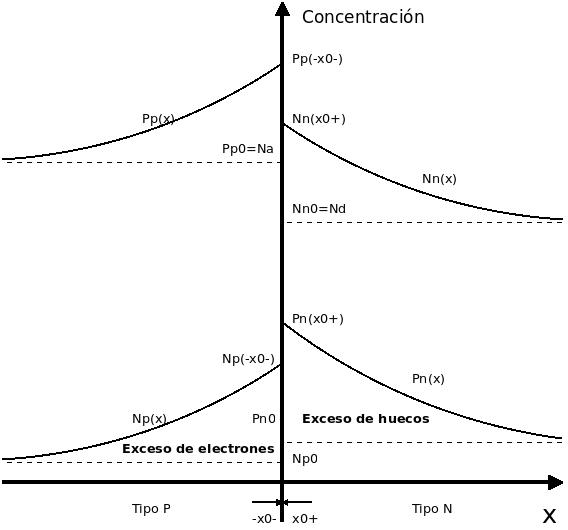
\includegraphics[scale=0.35]{Concentracion-Directa.jpeg}
							\caption{Concentración de portadores en la cercanía de la juntura PN en polarización directa}
						\end{center}
					\end{figure}							
				\end{minipage}
				\begin{minipage}[t]{0.4\textwidth}
					\begin{figure}[H]
						\begin{center}
							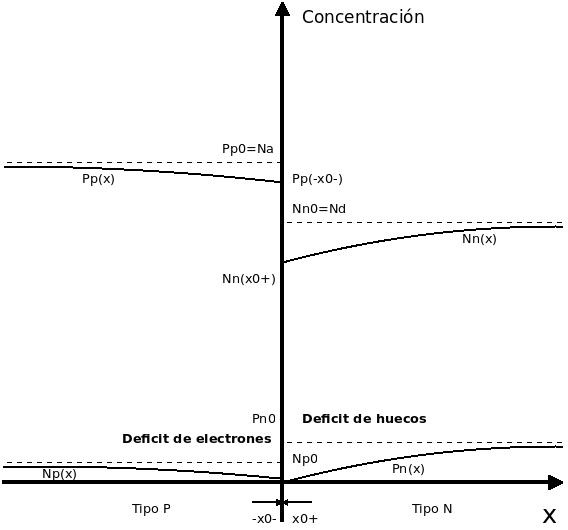
\includegraphics[scale=0.35]{Concentracion-Inversa.jpeg}
							\caption{Concentración de portadores en la cercanía de la juntura PN en polarización inversa}
						\end{center}
					\end{figure}							
				\end{minipage}
				
				Se desprecia cualquiera generación o recombinación térmica de portadores que pueda ocurrir dentro de la zona de vaciamiento, cuyo espesor es muy pequeño y los campos muy altos, acelerando casi siempre a los electrones desde el lado P, y a los huecos desde el lado N, para que atraviesen la capa en un intervalo muy pequeño en comparación con sus tiempos de vida medios. Al hacer esta simplificación, la corriente de juntura se puede evaluar determinando las corrientes de difusión de los portadores minoritarios en las fronteras de la zona de vaciamiento:
				
				\begin{center}
					$\displaystyle J_n(0) \cong J_n(-x_0^-)=-D_n\left(\frac{d n_p}{dx}\right)_{-x_0^-}=-\frac{n_{p0}D_n}{L_n}\left(e^{e\frac{V_0}{kT}}-1\right)$
					
					$\displaystyle J_p(0) \cong J_p(x_0^+)=-D_p\left(\frac{d p_n}{dx}\right)_{x_0^+}=\frac{p_{n0}D_p}{L_p}\left(e^{e\frac{V_0}{kT}}-1\right)$
				\end{center}
		
				La corriente eléctrica que cruza la juntura será:
				
				\begin{center}
					$\displaystyle I=e\left(J_p(0)-J_n(0)\right)=e\left(\frac{n_{p0}D_n}{L_n}+\frac{p_{n0}D_p}{L_p}\right)\left(e^{e\frac{V_0}{kT}}-1\right)$
					
					$\Downarrow$
					
					$\displaystyle I_0=e\left(J_{ng}+J_{pg}\right)=e\left(\frac{n_{p0}D_n}{L_n}+\frac{p_{n0}D_p}{L_p}\right)=e n_i^2\left(\frac{D_n}{p_{p0}L_n}+\frac{D_p}{n_{n0}L_p}\right)$
				\end{center}
		
				La corriente de saturación se puede reducir mediante el uso de un material con impurificación relativamente fuerte en la región N y P, y también haciendo que el tiempo de vida de los portadores en exceso sea lo más grande posible en ambas regiones.\\
	
			\subsection{Experiencia de Haynes-Schockley}
				
				Realizado originalmente para medir la movilidad de arrastre de huecos y electrones en cristales semiconductores con precisión y de un modo directo. Presenta un gran interés debido a que fue la primera medición directa de la velocidad de arrastre de portadores de carga, también es muy instructivo para dilucidar el comportamiento de transporte de portadores en exceso en semiconductores. Además de demostrar las características básicas del funcionamiento del transistor, ya que el circuito de Haynes-Shockley es, en efecto, un tipo de transistor.
				
				\begin{figure}[H]
					\begin{center}
						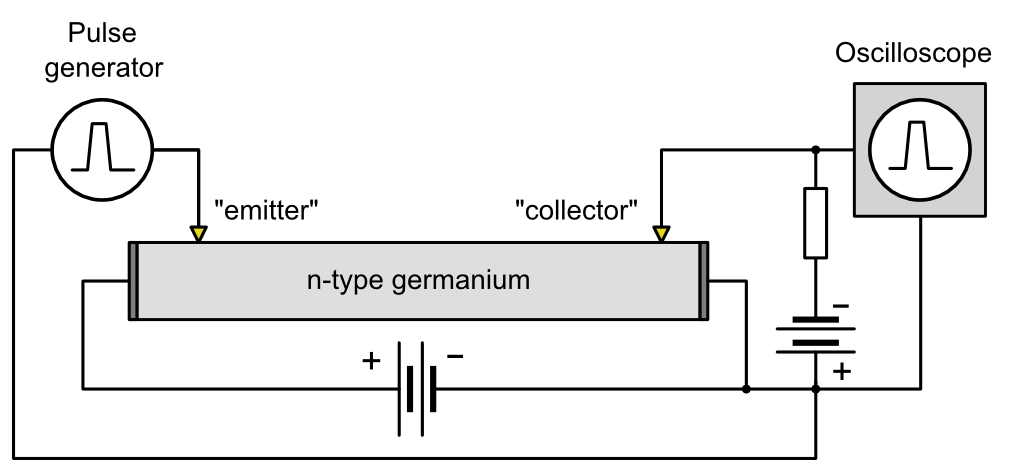
\includegraphics[scale=0.45]{Haynes-Shockley.png}
						\caption{Diagrama esquemático del experimento de Haynes-Shockley}
					\end{center}
				\end{figure}					
							
				Se inyecta un exceso de portadores minoritarios al cristal por el emisor y se recogen por el colector mediante un contacto de puntas de prueba metálicas. La misma actúa como un contacto rectificador; cuando se polariza de tal manera que atraiga hacia ella a los portadores minoritarios, actuará como un colector de portadores minoritarios vaciando la región del cristal adyacente a ella de estos portadores, hasta que se llega a un estado estacionario en que los portadores minoritarios se difunden desde el interior del cristal con la suficiente rapidez para satisfacer el déficit causado por su desaparición en las puntas de prueba. En estas condiciones (\textbf{polarización inversa}), esta corriente de portadores minoritarios es la única que puede fluir por la punta de prueba y, puesto que es muy pequeño el abastecimiento de portadores minoritarios del cristal, el flujo de la corriente se reduce mucho y es relativamente independiente del voltaje de polarización, ya que al suministro de portadores minoritarios no le afecta el cambio del voltaje de polarización inversa.\\
				
				Cuando el voltaje de polarización se invierte para atraer a portadores mayoritarios a la punta de prueba, además del flujo de éstos hacia ella, se inyecta un exceso de  portadores minoritarios a la muestra en el contacto de puntas, la corriente fluye con facilidad y se pueden alcanzar flujos de corriente relativamente grandes con pequeños voltajes de polarización, de un modo aproximadamente exponencial. Este modo se denomina \textbf{polarización directa}	
							
				\begin{minipage}[t]{0.4\textwidth}
					\begin{figure}[H]
						\begin{center}
							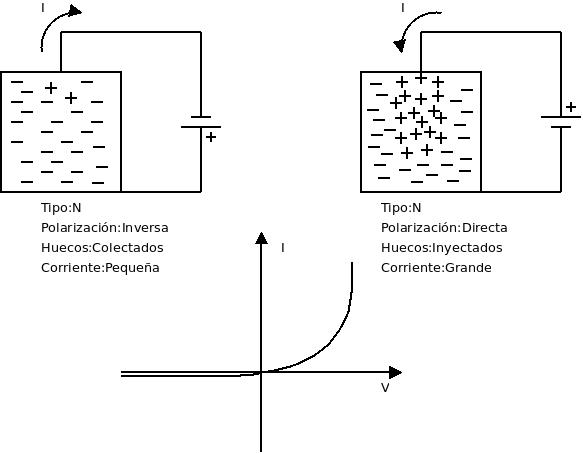
\includegraphics[scale=0.35]{Rectificador-N.jpeg}
							\caption{Rectificador con puntas tipo N}
						\end{center}
					\end{figure}		
				\end{minipage}
				\begin{minipage}[t]{0.4\textwidth}
					\begin{figure}[H]
						\begin{center}
							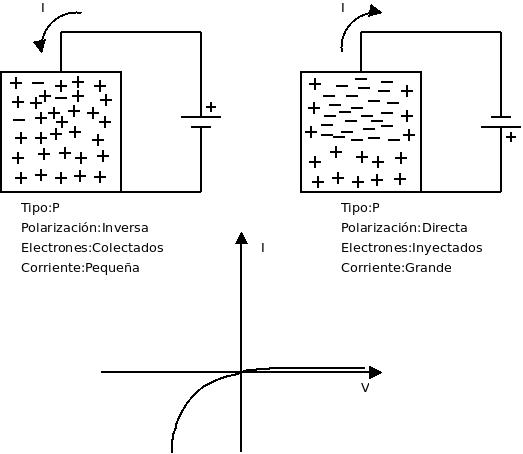
\includegraphics[scale=0.35]{Rectificador-P.jpeg}
							\caption{Rectificador con puntas tipo P}
						\end{center}
					\end{figure}		
				\end{minipage}
				
		\section{Sistema Metal-Semiconductor}
		
			Considerando las junturas metal-semiconductor rectificantes, o \emph{diodos de barrera Schottky}. En la mayoría de los casos, los contactos rectificantes se hacen sobre semiconductores de tipo n, por esta razón nos concentraremos en este tipo de diodo.

			\subsection{Características cualitativas.}

				Los diagramas de bandas ideales para un metal y un semiconductor de tipo N, antes de hacer contacto, se muestran en la figura \ref{Diagrama de bandas de un metal y un semiconductor sin contacto}. El nivel de vacío se usa como un nivel de referencia (es cuando los electrones son completamente libres).

				\begin{figure}[H]
					\begin{center}
						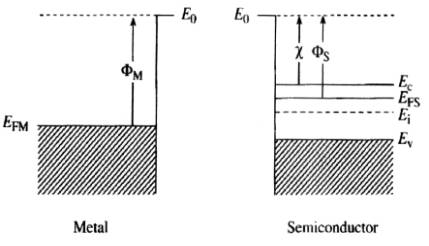
\includegraphics[width=0.7\textwidth]{metalsemiconductorsincontacto.jpeg}
						\caption{Diagrama de bandas de un metal y un semiconductor sin contacto}
						\label{Diagrama de bandas de un metal y un semiconductor sin contacto}
					\end{center}
				\end{figure}

				El parámetro $\phi _{m}$ es la función de trabajo del metal (medida en volts), $\phi _{s}$ es la función de trabajo del semiconductor y $\chi$ es la afinidad electrónica. El diagrama de bandas ideal, en equilibrio térmico, para la juntura metal-semiconductor en esta situación es el que se presenta en la figura \ref{Diagrama de bandas de un metal y un semiconductor con contacto}, donde \textbf{a)} y \textbf{c)} ocurren un instante después de la formación de la juntura, con \textbf{b)} y \textbf{d)} son las condiciones de equilibrio de ambos estados respectivamente.
			
			\begin{figure}[H]
				\begin{center}
					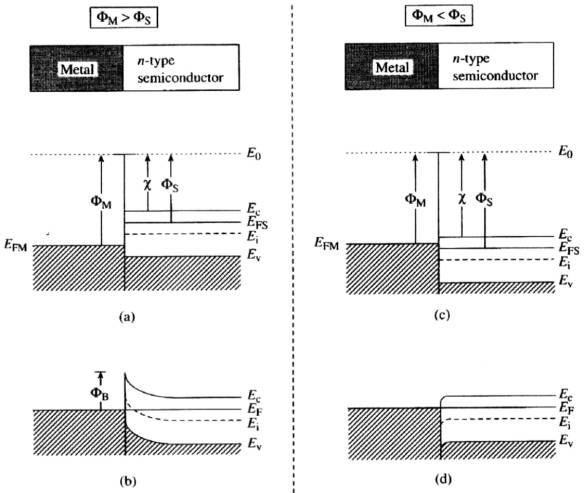
\includegraphics[width=0.7\textwidth]{metalsemiconductorencontacto.png}
					\caption{Diagrama de bandas de un metal y un semiconductor con contacto}
					\label{Diagrama de bandas de un metal y un semiconductor con contacto}
				\end{center}
			\end{figure}

			Antes de hacer contacto, la energía de Fermi en el semiconductor está por encima de la energía de Fermi en el metal. Para que la energía de Fermi se vuelva constante, a través del sistema, en equilibrio térmico, los electrones del semiconductor deben fluir a los estados vacíos del metal (recordar que la energía de Fermi es indicativo de todos los estados ocupados a $0K$, entonces, si la energía de Fermi en el semiconductor es mayor, quiere decir que, en el metal, hay estados de energía menor que no han sido ocupados, y como ley fundamental, las partículas ocupan los estados de menor energía, los electrones del semiconductor fluirán hacia el metal). Cuando esto suceda, átomos donores permanecerán en el semiconductor, creando una zona de carga espacial.\\

			El parámetro $\phi_{B_0}$ es la altura ideal de la barrera del contacto semiconductor, es la barrera de potencial que ven los electrones del metal al intentar moverse hacia el semiconductor. Esta barrera se conoce como la \emph{barrera de Schottky} y viene dada, idealmente, por $\phi_{B_0}=\phi_{m}-\chi$\\

			En el lado del semiconductor, $V_{bi}$ es la barrera de potencial interna. Esta barrera, similar al caso de la juntura pn, es la barrera que ven los electrones en la banda de conducción del semiconductor, para moverse al metal. La barrera de potencial interna viene dada por $V_{bi}=\phi_{B_0}-\phi_n$ o que hace que $V_{bi}$ sea, en parte, función del dopaje, como en el caso de la juntura PN.\\

			Si aplicamos una tensión positiva al semiconductor respecto del metal, la altura de la barrera semiconductor-a-metal se incrementa, mientras que $\phi_{B_0}$ permanece constante en este caso ideal. Esta es la condición de polarización inversa. Si una tensión positiva es aplicada al metal respecto del semiconductor, $V_{bi}$ se reduce mientras que, $\phi _{B_0}$ permanece esencialmente constante. En este caso, los electrones pueden fluir fácilmente del semiconductor al metal dado que la barrera se redujo. Esta es la condición de polarización directa. En la figura \ref{Diagrama de bandas de la juntura metal-semiconductor} podemos observar los diagramas de bandas para cada caso, donde $V_R$ es la tensión aplicada en polarización inversa y $V_a$ es la tensión aplicada en polarización directa.

			\begin{figure}[H]
				\begin{center}
					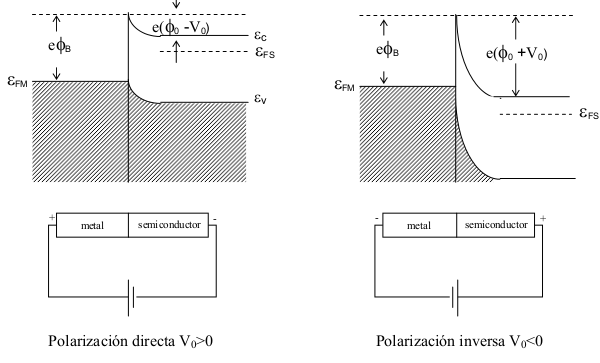
\includegraphics[width=0.8\textwidth]{metalsemiconductorpolarizacion.png}
					\caption{Diagrama de bandas de la juntura metal-semiconductor}
					\label{Diagrama de bandas de la juntura metal-semiconductor}
				\end{center}
			\end{figure}

			Los diagramas de bandas de la figura \ref{Diagrama de bandas de la juntura metal-semiconductor} son bastante parecido a aquellos de la juntura PN. Dada esta similitud, esperaremos que la característica tensión-corriente del diodo de barrera Schottky sea parecida al comportamiento exponencial de la característica del diodo de juntura pn. Sin embargo, en el caso del diodo de barrera Schottky, la corriente se genera por el flujo de los portadores mayoritarios. En polarización directa, la barrera que ven los electrones se reduce, con lo cual estos portadores mayoritarios pueden fluir más fácilmente del semiconductor al metal. Esta corriente de polarización directa va en la dirección del metal al semiconductor (al revés que el movimiento de los electrones), y también es una función exponencial de la tensión de polarización directa, $V_a$.

			\subsection{Propiedades de la juntura ideal.}

			Se pueden determinar las propiedades electrostáticas de la juntura metal-semiconductor (M-SC) de la misma forma que se determinaron para el diodo de juntura PN. El campo eléctrico en la zona espacial de carga viene dado por la ecuación de Poisson
			
			\begin{center}
				$\frac{dE}{dx}=\frac{\rho(x)}{\varepsilon _{s}}$
			\end{center}

			donde $\rho (x)$ es la densidad volumétrica de carga y $\varepsilon_{s}$ es la permitividad del semiconductor. Si asumimos que el dopaje del semiconductor es uniforme, entonces, al integrar la ecuación anterior, obtenemos
			
			\begin{center}
				$E=\int \frac{eN_d}{\varepsilon_s}dx=\frac{eN_d x}{\varepsilon_s}+C_1$
			\end{center}
			
			donde $C_1$ es la constante de integración. El campo eléctrico es cero en el borde de la zona de carga espacial, del lado del semiconductor, ($x=x_n$ en la figura \ref{Diagrama de bandas de la juntura metal-semiconductor}), con lo cual, la constante de integración es
		
			\begin{center}	
				$C_1=-\frac{eN_d x_n}{\varepsilon_s}$
			\end{center}
			
			y el campo eléctrico puede ser escrito como
			
			\begin{center}
				$E=-\frac{eN_d}{\varepsilon_s}(x_n-x)$
			\end{center}

			que es una función lineal de la distancia, para un semiconductor dopado uniformemente y alcanza un máximo (en módulo) para la interfaz metal-semiconductor. Dado que el campo eléctrico es cero en el interior de un metal, una carga superficial negativa debe existir en el metal, en la interfaz (esto es así porque el campo eléctrico fue originado en los átomos donores de la zona de carga espacial, que son positivos; y como el campo eléctrico nace en carga positiva y muere en carga negativa, debe haber carga negativa en la superficie de la interfaz que haga que el campo eléctrico sea cero dentro del metal).

			El ancho de la región de carga espacial, $W$, puede ser calculado como hicimos para la juntura PN. El resultado es idéntico al de una juntura unilateral $P^+N$. Para el semiconductor dopado uniformemente, tenemos
			
			\begin{center}
				$W=x_n=\left( \frac{2 \varepsilon_s (V_{bi}+V_R)}{eN_d} \right)^{\frac{1}{2}}$
			\end{center}
			
			donde $V_R$ es la magnitud de la tensión aplicada en polarización inversa. En este caso, también se utiliza la aproximación de la juntura abrupta.

			Se puede determinar, también, una capacitancia de juntura en el mismo modo que se determinó para la juntura pn. Tenemos que
			
			\begin{center}
				$C^\prime=eN_d \frac{dx_n}{dV_R}=\left( \frac{e \varepsilon_s N_d}{2 (V_{bi}+V_R)} \right)^{\frac{1}{2}}$
			\end{center}
			
			donde $C^\prime$ es la capacitancia por unidad de área. Si elevamos al cuadrado la inversa de esta última ecuación, obtenemos
			
			\begin{center}
				$\left( \frac{1}{C^\prime} \right)^2=\frac{2(V_{bi}+V_R)}{e \varepsilon_s N_d}$
			\end{center}
			
			Podemos utilizar esta última ecuación para obtener, en una primera aproximación, la barrera de potencial interna, $V_{bi}$, y la pendiente de la curva y encontrar la concentración $N_d$. Podemos calcular el potencial $\phi _n$, teniendo la concentración $N_d$ con $\phi_n=-\dfrac{kT}{e} \ln \left( \dfrac{N_d}{n_i} \right)$, luego determinar el potencial de Schottky, $\phi_{B_0}$.

			\paragraph{}

				\scriptsize No se incluyen efectos no ideales ni función potencial en la juntura. Para función potencial en la juntura recurrir a las diapositivas de Ozols.

			\normalsize

			\subsection{Relación tensión-corriente.}

			La corriente en una juntura M-SC se debe, mayormente, a los portadores mayoritarios de carga, caso contrario a la juntura pn. El proceso básico, en un contacto rectificante con un semiconductor de tipo n, es el transporte de electrones a través de la barrera de potencial, que se puede describir usando la teoría de emisión termoiónica.\\

			Las características de la emisión termoiónica son obtenidas usando las suposiciones de que la altura de la barrera es mucho mayor a $kT$, de tal forma que la aproximación de Maxwell-Boltzmann sea válida y que el equilibrio térmico no se ve afectado por este proceso. En la figura \ref{Diagrama de bandas de la juntura metal-semiconductor} podemos observar una barrera unidimensional con una tensión de polarización directa aplicada, $V_{a}$, y también se pueden observar dos componentes de la densidad de corriente.\\

			La corriente $J_{s \rightarrow m}$ es la densidad de corriente del electrón debida al flujo de electrones del semiconductor al metal; y la corriente $J_{m \rightarrow s}$ es la densidad de corriente debida a electrones que fluyen del metal al semiconductor. Los subíndices de las densidades de corriente indican la dirección del flujo de electrones. La dirección convencional de corriente es opuesta al flujo de los electrones.\\

			La densidad de corriente $J_{s \rightarrow m}$ es una función de la concentración de electrones que tienen velocidades en dirección $x$ lo suficientemente altas para tener energía capaz de superar la barrera. Podemos escribir

			\begin{center}
				$J_{s \rightarrow m}=e \int_{\epsilon^\prime_c}^{\infty} v_x dn$
			\end{center}

			donde $\epsilon^\prime_c$ es la energía mínima requerida para la emisión termoiónica hacia el metal, $v_x$ es la velocidad de los portadores en la dirección del transporte y $e$ es la magnitud de la carga electrónica. La concentración incremental de electrones viene dada por
			
			\begin{center}
				$dn = g_c(\epsilon)f_F(\epsilon) d\epsilon$
			\end{center}
			
			donde $g_c(\epsilon)$ es la densidad de estados en la banda de conducción y $f_F(\epsilon)$ es la función de probabilidad de Fermi-Dirac. Suponiendo que la aproximación de Maxwell-Boltzmann es válida, podemos escribir
			
			\begin{center}
				$dn=\frac{4 \pi (2m^{\ast}_n)^{\frac{3}{2}}}{h^3} \cdot \sqrt{\epsilon-\epsilon_c} \cdot e^{-\frac{\epsilon-\epsilon_F}{kT}} d\epsilon$
			\end{center}

			Si toda la energía de los electrones, superior a $\epsilon _c$ la suponemos energía cinéticda, entonces tenemos que
			
			\begin{center}
				$\frac{1}{2} m_n^{\ast} v^2=\epsilon-\epsilon_c$
			\end{center}
			
			La densidad de corriente neta en una juntura M-SC se puede escribir como
			
			\begin{center}
				$J=J_{s \rightarrow m}-J_{m \rightarrow s}$
			\end{center}
			
			que queda definida positiva en la dirección del metal al semiconductor. Encontramos, entonces, que

			\begin{center}
				$J=A^{\ast}T^2 e^{-\frac{e\phi _{B_0}}{kT}} (e^{\frac{eV_a}{kT}} -1)$
			\end{center}

		donde $A^{\ast} \equiv \frac{4 \pi e m_n^{\ast} k^2}{h^3}$ y este parámetro se llama la constante efectiva de Richardson para la emisión termoiónica.

		Esta última ecuación se puede escribir de la forma usual del diodo como
		
		\begin{center}
			$J=J_{sT}(e^{\frac{eV_a}{kT}}-1)$
		\end{center}
		
		donde $J_{sT}$ es la densidad de corriente de saturación inversa y viene dada por
		
		\begin{center}
			$J_{sT}=A^{\ast}T^2 e^{-\frac{e \phi _{B_0}}{kT}}$
		\end{center}

		\paragraph{}

			\scriptsize No incluye la comparación entre el diodo de barrera Schottky y el diodo de juntura pn.

			\normalsize

		\subsection{Contactos óhmicos en junturas metal-semiconductor.}

			Deben existir contactos entre los dispositivos semiconductores o los circuitos integrados y el mundo exterior. Estos contactos se hacen mediante \emph{contactos óhmicos}. Los contactos óhmicos son junturas M-SC pero que no son rectificantes. Un contacto óhmico es una juntura de baja resistencia que proporciona conducción en ambos sentidos, entre el metal y el semiconductor. Idealmente, la corriente a través del contacto óhmico es una función lineal de la tensión aplicada y la tensión aplicada debe ser muy pequeña. Existen dos tipos de contactos óhmicos posibles: el primero es una barrera ideal no-rectificante, y el segundo es un contacto túnel. Definiremos una resistencia de contacto específica que se usa para caracterizar a los contactos óhmicos.

		\subsection{Barreras ideales no-rectificantes.}

			Para conseguir equilibrio térmico en una juntura M-SC ideal, los electrones fluirán desde el metal a los estados de menor energía, libres en el semiconductor, lo que hace que la superficie del semiconductor sea más de tipo n. Este exceso de electrones en el semiconductor de tipo n existe, esencialmente, como una densidad de carga superficial. Si una tensión positiva es aplicada al metal, respecto del semiconductor, no existe ninguna barrera para los electrones que fluyen del semiconductor al metal. Si una tensión positiva es aplicada al semiconductor, respecto del metal, la altura de la barrera efectiva para los electrones fluyendo del metal al semiconductor será, aproximadamente, $\phi_{B_0}=\phi_n$, que es considerablemente pequeña para un semiconductor altamente dopado. Para esta polarización, los electrones puede fluir fácilmente del metal al semiconductor.
			
			En una juntura ideal no-rectificante entre un metal y un semiconductor de tipo p. La figura 6a muestra los niveles de energía antes del contacto para el caso donde $\phi_m > \phi_s$. Cuando se realiza el contacto, los electrones del semiconductor fluirán en el metal para alcanzar el equilibrio térmico, dejando atrás mayor cantidad de estados vacíos o huecos. El exceso en la concentración de huecos hará que la superficie del semiconductor sea más tipo p. Los electrones del metal se pueden mover fácilmente a los estados vacíos en el semiconductor. Este movimiento de carga corresponde a huecos fluyendo del semiconductor al metal.

			\subsection{Contacto túnel}
			
			El ancho de la zona de carga espacial en una juntura M-SC rectificante es inversamente proporcional a la raíz cuadrada del dopaje del semiconductor. El ancho de la zona de vaciamiento disminuye a medida que aumenta la concentración de dopantes en el semiconductor; por lo tanto, como la concentración de dopantes aumenta, la probabilidad de tunelamiento a través de la barrera aumenta.

			La corriente de tunelamiento tiene la forma $J_t \sim e^{-\frac{e \phi_{B_0}}{E_{\infty}}}$, donde $E_{\infty}=\frac{e \hbar}{2} \sqrt{\frac{N_d}{\varepsilon_s m_n^{\ast}}}$. El tunelamiento aumenta exponencialmente con la concentración de dopantes.

			\subsection{Resistencia específica de contacto}

				Una figura de mérito de los contactos óhmicos es la resistencia específica de contacto, $R_{c}$. Este parámetro es definido como el inverso de la derivada de la densidad de corriente respecto de la tensión evaluada cuando no hay polarización. Es decir,
				
				\begin{center}
					$R_c=\left( \frac{\partial J}{\partial V} \right)^{-1} \rfloor_{V=0} \qquad [R_c]=\Omega\text{cm}^{2}$
				\end{center}
				
				Lo ideal es que $R_c$ sea lo más pequeño posible para un contacto óhmico.

				Para un contacto rectificante con una concentración moderadamente pequeña de dopantes, la relación tensión-corriente viene dada por la ecuación
				
				\begin{center}
					$J=A^{\ast}T^2 e^{-\frac{e\phi_{B_0}}{kT}}(e^{\frac{eV_a}{kT}} -1)$
				\end{center}
				
				La corriente por emisión termoiónica es dominante en estas junturas. En este caso, la resistencia específica de contacto es
						
				\begin{center}
					$R_c=\frac{\left( \dfrac{kT}{e} \right) e^{\frac{e \phi_{B_0}}{kT}}}{A^{\ast}T^2}$
				\end{center}
				
				La resistencia específica de contacto disminuye rápidamente a medida que disminuye la altura de la barrera.

				Para una juntura M-SC con una gran concentración de dopantes, los procesos de tuneleo dominan. Utilizando la ecuación de $J_{t}$ obtenemos
				
				\begin{center}
					$R_c \sim e^{\frac{2\sqrt{\varepsilon_s m^{\ast}_n}}{\hbar} \cdot \frac{\phi_{B_0}}{\sqrt{N_d}}}$
				\end{center}
				
				que muestra que la resistencia específica de contacto depende fuertemente del dopaje del semiconductor.

				La teoría para formar contactos óhmicos es bastante sencilla. Para obtener un buen contacto óhmico, necesitamos crear una barrera pequeña y usar un semiconductor altamente dopado en la superficie. Sin embargo, la tecnología actual para fabricar contactos óhimcos buenos y confiables, no es tan sencilla en la práctica como en la teoría. También resulta más difícil fabricar buenos contactos óhmicos en materiales que tienen un gran ancho de banda. En general, las barreras no son pequeñas en este tipo de materiales y, por lo tanto, deben usarse semiconductores altamente dopados en la superficie para formar un contacto túnel.

		\section{Sistema Metal-Óxido-Semiconductor (MOS)}
		
			Las junturas MOS son la base de los dispositivos semiconductores mas modernos. En principio el capacitor MOS es una pieza de estudio importante.\\
			
			Dado que genéricamente se usa como aislante el $SiO_2$ (Dióxido de Silicio), se habla de estructuras MOS (Metal Oxido Semiconductor) aunque también se denominan MIS (Metal Insulator Semiconductor).\\
			
			\begin{itemize}
				\item $t_{ox}$ es el espesor del aislante.
				\item $V_G$ es la tensión aplicada al metal. Por convención si el positivo se aplica al metal, es polarización directa. El metal es llamado \textbf{Gate} (\textit{compuerta}) ya que será el nombre del electrodo del transistor MOSFET cuando esta estructura MOS sea la base del mismo.
				\item El Metal: puede ser Aluminio o un semiconductor degenerado o semimetal (Silicio Policristalino).
				\item El Aislante (Insulator): puede ser SiO2 (Dioxido de Silicio) .
				\item El Semiconductor : Silicio (tipo p o tipo n).
			\end{itemize}
			
			Análizando en el caso de un substrato tipo P:\\
		
			\begin{minipage}[t]{0.4\textwidth}
				\begin{figure}[H]
						\begin{center}
							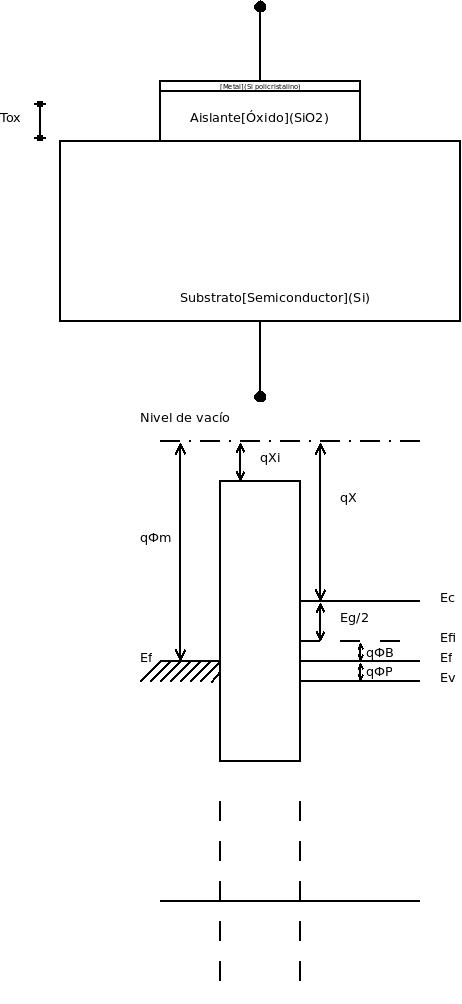
\includegraphics[scale=0.4]{MOS-esquema.jpeg}
							\caption{MOS sin tensión aplicada}
						\end{center}
					\end{figure}	
				\end{minipage}
				\begin{minipage}[t]{0.4\textwidth}		
					\begin{figure}[H]
						\begin{center}
							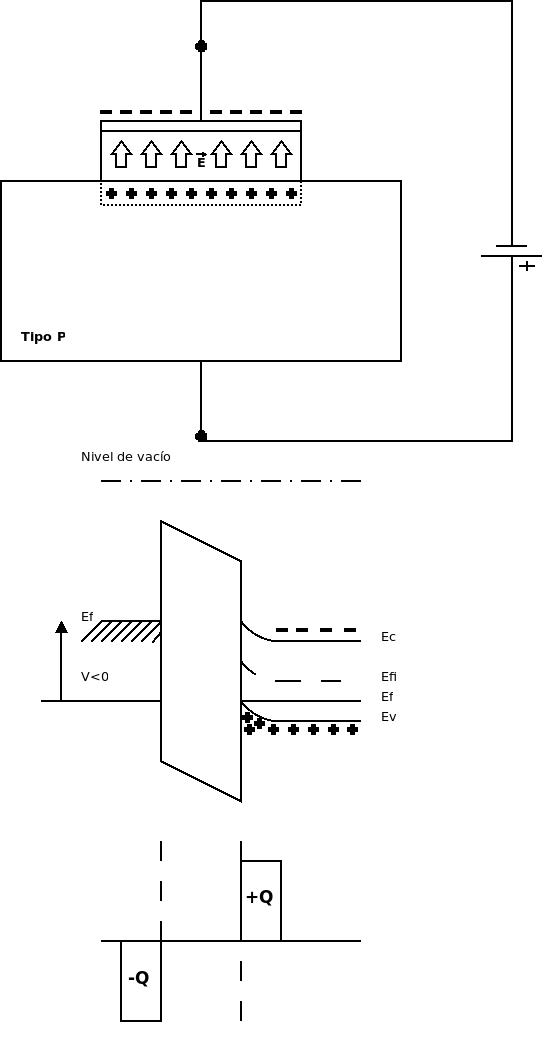
\includegraphics[scale=0.4]{MOS-Acum.jpeg}
							\caption{Acumulación, $V_{FB}<V_G<0$}
						\end{center}
					\end{figure}	
				\end{minipage}
				
				\begin{minipage}[t]{0.4\textwidth}	
					\begin{figure}[H]
						\begin{center}
							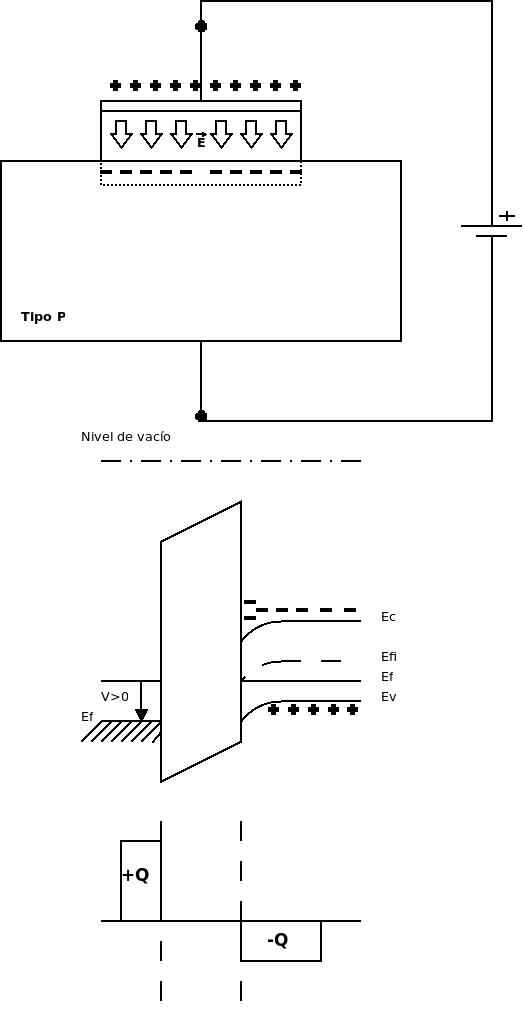
\includegraphics[scale=0.4]{MOS-Dep.jpeg}
							\caption{Vaciamiento, $V_{TH}>V_G>0$}
						\end{center}
					\end{figure}	
				\end{minipage}
				\begin{minipage}[t]{0.4\textwidth}	
					\begin{figure}[H]
						\begin{center}
							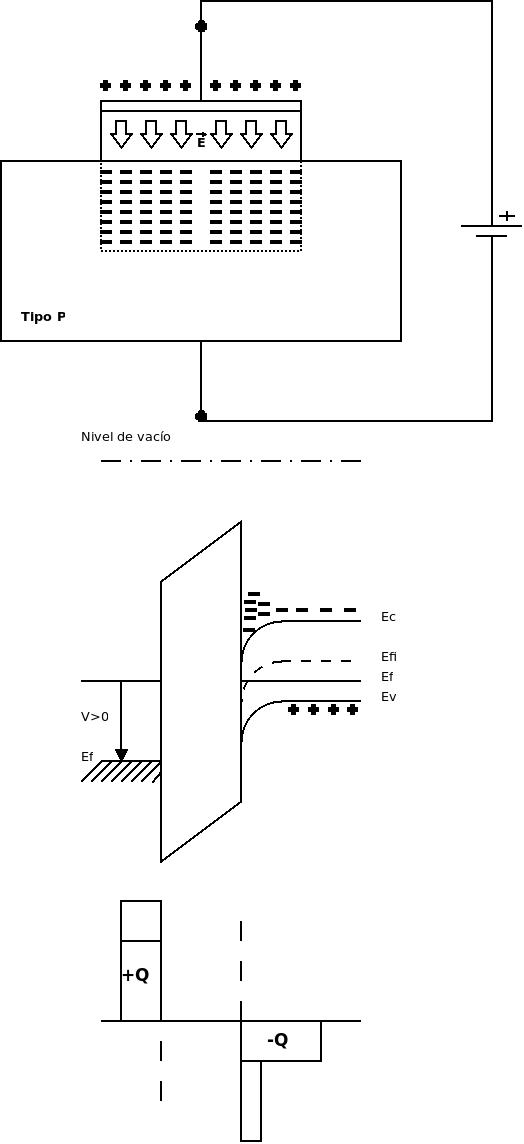
\includegraphics[scale=0.4]{MOS-Inv.jpeg}
							\caption{Inversión, $V_G>V_{TH}$}
						\end{center}
					\end{figure}	
				\end{minipage}	
				
				\textbf{Acumulación:} $V_G$ es negativa. El nivel de Fermi del metal se eleva respecto al $E_f$ del Semiconductor y en este último las bandas se curvan hacia arriba en la cercanía del óxido y $E_v$ se acerca a $E_f$, esto causa una acumulación de portadores mayoritarios cerca del óxido. También se puede ver como que los huecos son atraídos hacia la interfase con el óxido por el negativo del Gate. Aparece una carga negativa en el lado metal del capacitor para mantener la neutralidad.\\

				\textbf{Vaciamiento:} $V_G$ es positiva y pequeña. El nivel de Fermi del metal desciende respecto al $E_f$ del Semiconductor y en este las bandas se curvan hacia abajo en la cercanía del óxido y $E_v$ se aleja de $E_f$, esto causa un vaciado de portadores mayoritarios (huecos) cerca del óxido. También se puede ver que los huecos son repelidos de la interfase con el óxido por el positivo del Gate. Aparece una cantidad de carga de igual magnitud pero positiva en el lado metal del capacitor para mantener la neutralidad.\\

				\textbf{Inversión:} Si el valor de $V_G$ positivo se incrementa, aumenta la zona de vaciamiento de huecos y también la presencia de carga negativa en esa zona cercana al óxido. Esto se mantiene hasta que las bandas se curvan tanto hacia abajo (en la cercanía del óxido) que $E_{fi}$ se vuelve menor que $E_f$ . Cuando esto sucede todos los huecos se retiraron de las inmediaciones de la interface con el óxido y allí ahora hay muchos mas electrones en banda de conducción que huecos en banda de valencia. Se ha producido la inversión de la naturaleza del material en esa zona próxima al óxido. Tener en cuenta que esto no se produjo por dopaje sino por la aplicación de un campo eléctrico.\\
				
				La carga negativa en el semiconductor está formada no sólo por electrones en la banda de conducción sino por impurezas aceptoras ionizadas . Y nuevamente aparece una cantidad de igual cantidad de carga positiva en el lado metal del capacitor para mantener la neutralidad.
La inversión comienza cuando $E_{fi}=\frac{E_c-E_v}{2}$ cruza $E_f$.\\

				Si la concentración de electrones en la superficie próxima al óxido permanece pequeña se conoce como inyección débil. Si $V_G$ se incrementa de manera tal que la concentración de electrones iguala o aún supera a la de huecos en equilibrio térmico, se llega a una inversión fuerte.
Con $V_G \neq 0$, el nivel de Fermi ($E_f$) aparece quebrado en el óxido ya que al no haber portadores varía bruscamente. Y en el metal y el semiconductor permanece horizontal al no existir corriente.\\

			\subsection{MOSFET}
			
				\begin{figure}[H]
					\begin{center}
						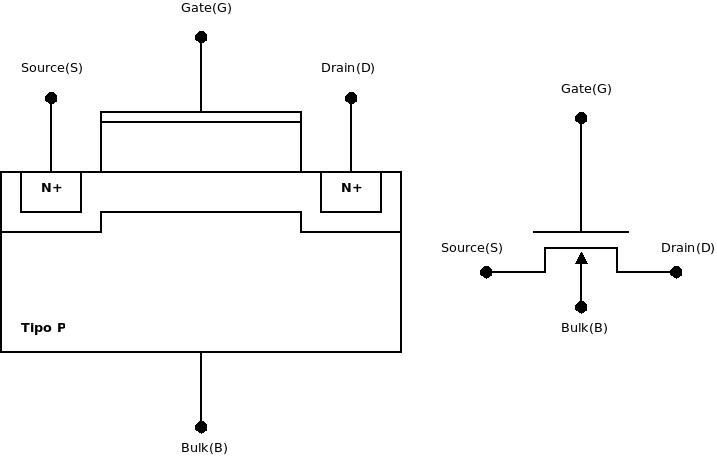
\includegraphics[scale=0.4]{N-MOSFET.jpeg}
						\caption{Estructura física del N-MOSFET}
					\end{center}
				\end{figure}	
				
			\subsubsection{Curvas características del transistor MOS(N o P) }
				
				Se definen los parámetros del transistor:
				
				\begin{itemize}
					\item $\mu$: Movilidad de los portadores ($\mu_n$ o $\mu_p$)
					\item $\epsilon$: Permitividad eléctrica del medio ($SiO_2$)
					\item $t_{ox}$: Espesor de la capa de óxido ($SiO_2$)
					\item $W$: Ancho del canal
					\item $L$: Longitud del canal
					\item $W/L$: Relación de aspecto
					\item $C_{ox}=\frac{\epsilon}{t_{ox}}$: Capacidad de puerta por unidad de área
					\item $K$: Factor dependiente del proceso de fabricación
				\end{itemize}						
				
				\begin{center}
					$\displaystyle \beta=\frac{\mu \epsilon}{t_{ox}}\left(\frac{W}{L}\right)=\mu C_{ox}\left(\frac{W}{L}\right)=K\left(\frac{W}{L}\right)$\\
				\end{center}				
				
				El transistor MOS presenta tres zonas de funcionamiento:\\
				
				\begin{enumerate}
					\item Zona de corte o subumbral:
						\begin{itemize}
							\item Se produce cuando: $0<|V_{GS}|<|V_{TH}|$
							\item No hay canal formado
								\begin{itemize}
									\item $V_{GS}$ por debajo de la tensión umbral.
									\item Transistor en \textit{OFF} o en corte. 
								\end{itemize}
							\item \boxed{I_{DS}=0}
							\item Modelo equivalente: circuito abierto.
						\end{itemize}
					\item Zona lineal u óhmica (no saturada).
						\begin{itemize}
							\item Se produce cuando: $|V_{DS}|<|V_{GS}-V_{TH}|$
							\item \boxed{\displaystyle I_{DS}=K\left(\frac{W}{L}\right)\left[(V_{GS}-V_{TH})-\frac{V_{DS}}{2}\right]V_{DS}}
							\item Modelo equivalente: Resistencia entre Source y Drain, que será tanto menor cuanto mayor sea la tensión en puerta $V_{GS}$:
								\begin{center}
									$\displaystyle \frac{V_{DS}}{I_{DS}}=\frac{1}{K\left(\frac{W}{L}\right)\left[(V_{GS}-V_{TH})-\frac{V_{DS}}{2}\right]} \cong \frac{L}{KW\left[V_{GS}-V_{TH}\right]}=R$
								\end{center}
							\item La movilidad de los huecos $\mu_p$ es notoriamente menor que la de los electrones $\mu_n$ para el silicio. 
							\item La ganancia $\beta$ será casi tres veces menor en un transistor P con respecto al N.
							\item La resistencia de canal R será casi tres veces mayor para las mismas relaciones de aspecto y proceso tecnológico en un transistor tipo P respecto al tipo N.
							\item Los transistores PMOS son sensiblemente más resistivos.
							\item Los transistores PMOS son más lentos en la conmutación de una capacidad.
						\end{itemize}
					\item Zona de saturación.
						\begin{itemize}
							\item Se produce cuando: $|V_{DS}|>|V_{GS}-V_{TH}|$
							\item $\displaystyle I_{DS} \approx I_{sat}=cte$
							\item Este comportamiento es una consecuencia de la aparición de un fenómeno conocido como \textit{estrangulación del canal} o \textit{pinch-off}.
							\begin{itemize}
								\item Existe un campo eléctrico $\vec{E}_G$ entre Gate y Bulk cuando $V_{GS}>V_{TH}$
								\item Existe un campo eléctrico $\vec{E}_D$ entre Drain y Source.
									\begin{itemize}
										\item Si $V_{DS}=0$, $\vec{E}_D=0$
										\item Si $V_{DS}<(V_{GS}-V_{TH})$, $\vec{E}_D$ es débil. El perfil del canal se va estrechando en dirección al Drain, dado que la intensidad del campo $\vec{E}_G$ se va haciendo menor a medida que nos acercamos al Drain.
										\item Si $V_{DS}>(V_{GS}-V_{TH})$, $\vec{E}_D$ es fuerte. En esta zona, a medida que $V_{DS}$ se hace más grande, mayor será la zona estrangulada del canal pero a su vez el campo $\vec{E}_D$ será más intenso. El nivel de corriente $I_{DS}$ se mantiene prácticamente constante, es decir, alcanza su nivel de saturación ($I_{sat}$).
									\end{itemize}
								\end{itemize}									
							\item La línea de separación entre la zona lineal y la zona de saturación se alcanza cuando: $V_{DS}=V_{GS}-V_{TH}$
							\item \boxed{\displaystyle I_{DS}=\left[\frac{\beta(V_{GS}-V_{TH})}{2}\right](V_{GS}-V_{TH})=\beta \left[V_{DS}-\frac{V_{DS}}{2}\right] V_{DS}=\frac{\beta(V_{GS}-V_{TH})^2}{2}=\frac{\beta V_{DS}^2}{2} \cong cte}
							\item Debido a la reducción efectiva que experimenta el canal en la zona saturada, la expresión analítica utilizada para esta zona tiene la forma: $\displaystyle I_{DS}^{sat}=\frac{\beta V_{DS}^2}{2}(1+\lambda V_{DS})$, aunque usualmente se desprecia $\lambda$ por ser muy pequeño.
							\item Se tiene una resistencia equivalente $\displaystyle r_0=\left(\frac{\partial I_{DS}}{\partial V_{DS}}\right)^{-1} \approx \frac{1}{\lambda I_{DS}}$. Cuando $\lambda$ es muy pequeño y se desprecia, $r_0 \to \infty$.
							\item Modelo equivalente: Fuente de corriente $I_{DS}=I_{DS}^{sat}$ en paralelo con $r_0$, ambos entre Drain y Souce.
						\end{itemize}
				\end{enumerate}
						
				\begin{figure}[H]
					\begin{center}
						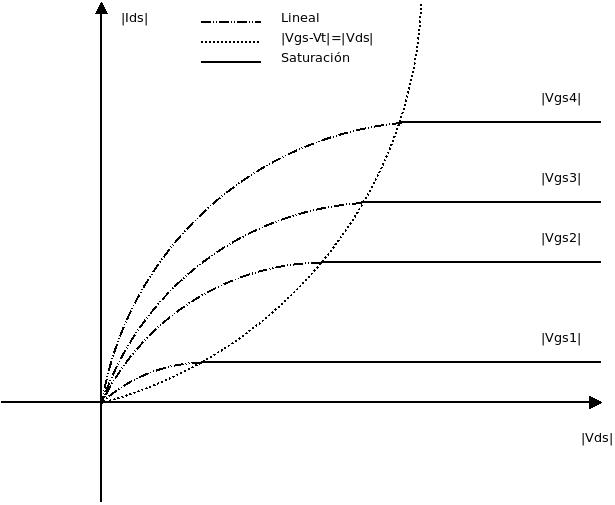
\includegraphics[scale=0.5]{Curvas-MOS.jpeg}
						\caption{Corriente $|I_{ds}|$ vs tensión $|V_{DS}|$ para NMOS y PMOS}
					\end{center}
				\end{figure}					
				
				\begin{figure}[H]
					\begin{center}
						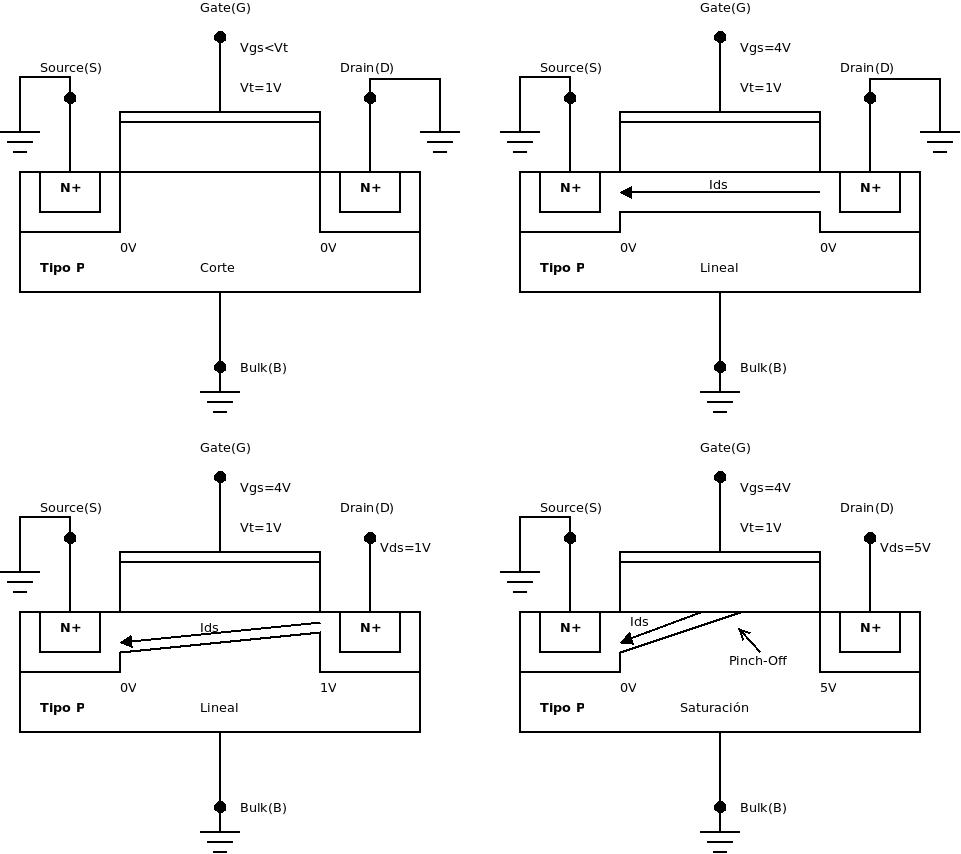
\includegraphics[scale=0.45]{N-MOS-modos.jpeg}
						\caption{Modos de funcionamiento del NMOS}
					\end{center}
				\end{figure}	
				
				\begin{figure}[H]
				
				
				\begin{tabular}{|c|c|c|c|c|}
						\hline & General & NMOS & PMOS & Equivalente \\ 
						\hline Corte & $0<|V_{GS}|<|V_{TH}|$ & $0<V_{GS}<V_{TH}$ & $0>V_{GS}>V_{TH}$ & 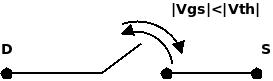
\includegraphics[scale=0.4]{Eq1.jpeg} \\ 
						\hline Lineal & $\begin{Bmatrix} |V_{DS}|<|V_{GS}-V_{TH}| \\ |V_{GS}|>|V_{TH}| \end{Bmatrix}$ & $\begin{Bmatrix} V_{DS}<V_{GS}-V_{TH} \\ V_{GS}>V_{TH} \end{Bmatrix}$ & $\begin{Bmatrix} V_{DS}>V_{GS}-V_{TH} \\ V_{GS}<V_{TH} \end{Bmatrix}$ & 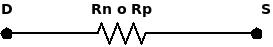
\includegraphics[scale=0.4]{Eq2.jpeg}\\ 
						\hline Saturación & $\begin{Bmatrix} |V_{DS}|>|V_{GS}-V_{TH}| \\ |V_{GS}|>|V_{TH}| \end{Bmatrix}$ & $\begin{Bmatrix} V_{DS}>V_{GS}-V_{TH} \\ V_{GS}>V_{TH} \end{Bmatrix}$ & $\begin{Bmatrix} V_{DS}<V_{GS}-V_{TH} \\ V_{GS}<V_{TH} \end{Bmatrix}$ & 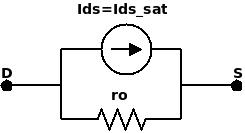
\includegraphics[scale=0.4]{Eq3.jpeg}\\ 
						\hline 
					\end{tabular} 
					\caption{Condiciones de aplicación}	
				\end{figure}
	
		\section{Transistor Bipolar de Juntura (TBJ)}
		
			El TBJ es de naturaleza bipolar, pues la corriente producida es debido al aporte de los electronesy de los huecos. Consiste en
\textbf{dos junturas PN} y posee tres terminales los que son llamados \textbf{Emisor(E)}, \textbf{Base(B)} y \textbf{Colector(C)}. El TBJ puede ser tipo \textit{NPN} o \textit{PNP}, la flecha indica la dirección normal de la corriente y define la polaridad de la tensión base-emisor. No es un dispositivo simétrico, pues intercambiando el emisor por el colector se obtienen resultados distintos.\\
		
			Sea el TBJ npn, éste considera una región N de volumen intermedio de alto dopamiento, una región P muy delgada de pequeño volumen de bajo dopamiento, y una región N de gran volumen de dopamiento intermedio. Para establecer su funcionamiento primero se polariza sólo la \textbf{juntura BE}, dejando el colector abierto. La juntura está \textbf{polarizada en directa}, luego se produce un \textbf{flujo de electrones desde el emisor a la base}, pero también fluirán \textbf{huecos en menor cantidad desde la base al emisor}. La corriente $I_E$ se produce por la suma de los electrones mayoritarios y huecos mayoritarios inyectados por el emisor y la base respectivamente. La corriente entre la base y el emisor será $I_E$ . Dado que la base es muy delgada, no soporta grandes corrientes.\\
		
			Polarizando solamente la \textbf{juntura CB}, dejando el emisor abierto, la juntura PN está \textbf{polarizada en inversa}, luego sólo existe movimiento de portadores minoritarios (huecos) del colector y los electrones minoritarios de la base, produciendo una corriente inversa de saturación llamada $I_{CB0}$, entre C y B.\\

				\begin{figure}[H]
					\begin{center}
						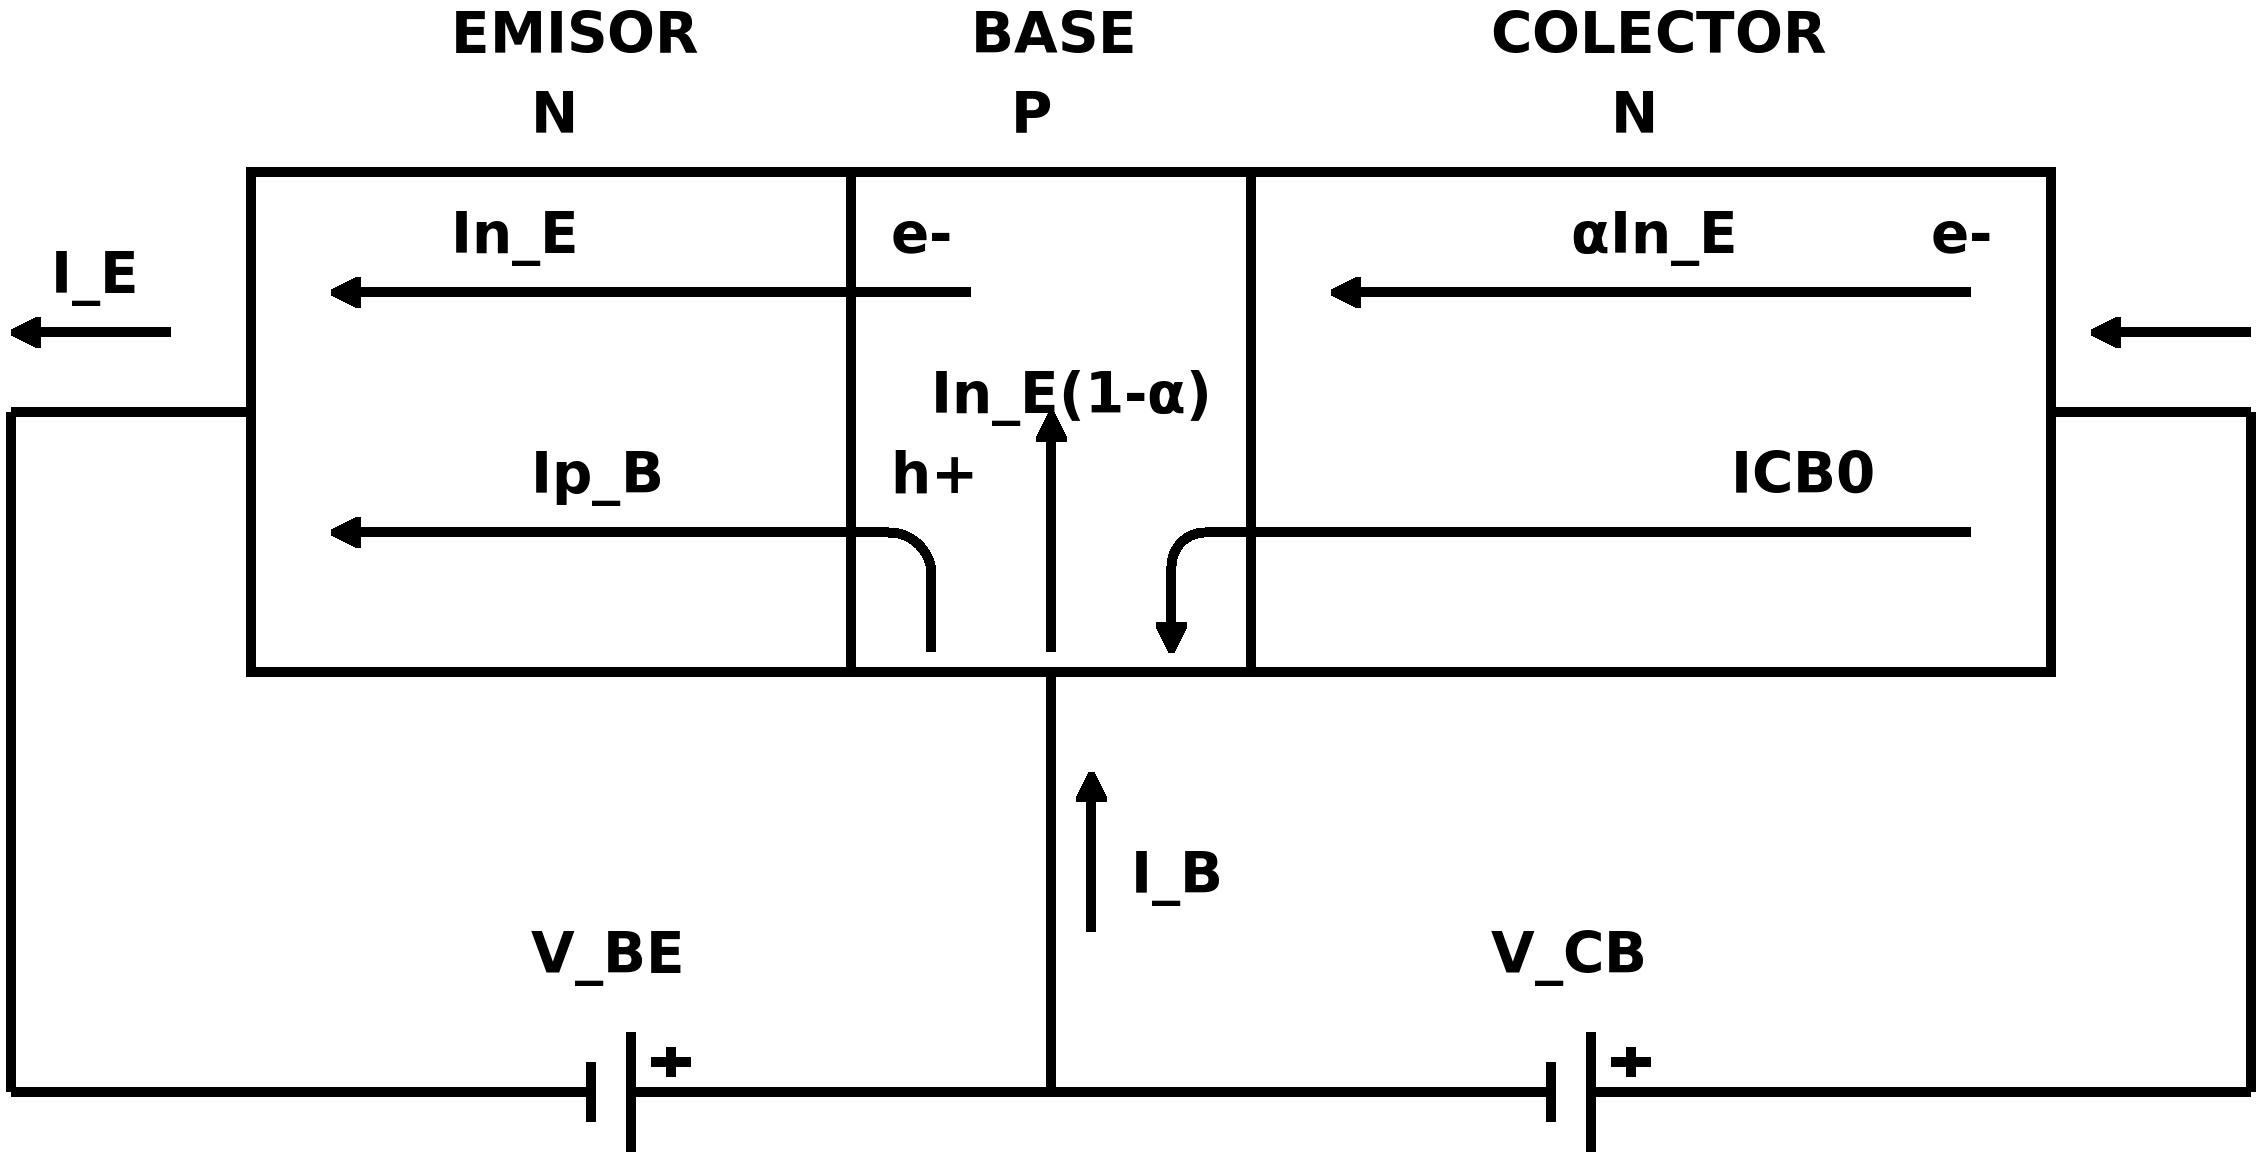
\includegraphics[scale=0.1]{NPN.jpeg}
						\caption{Estructura NPN polarizada}
					\end{center}
				\end{figure}	
				
			Al polarizar ambas junturas, los electrones mayoritarios inyectados por el emisor atraviesan la base llegando al colector, un pequeño porcentaje se recombina en la base con los huecos mayoritarios aportados por ésta. así, la corriente por el emisor debido a los electrones mayoritarios será $I_{n_E}$, pero la corriente en el colector debido a estos portadores será $\alpha I_{n_E}$; donde $\alpha$ es un número menor que 1, dado que parte de los electrones se recombinan en la base.\\
		
			Así, la corriente del emisor $I_E$ , será función de la corriente producida por los portadores mayoritarios (electrones) y la corriente debida a los portadores mayoritarios (huecos) inyectados por la base: 
		
			\begin{center}
				$I_E=I_{p_B}+I_{n_E}$
			\end{center}
		
			La corriente que se desvía a la base será $(1-\alpha)I_{n_E}=I_{n_R}$; luego la corriente en la base será la corriente de los huecos mayoritarios de la base mas la corriente $I_{n_R}$ menos la corriente $I_{CB0}$:
		
			\begin{center}
				$I_B=I_{p_B}+I_{n_R}-I_{CB0}$
			\end{center}
		
			Finalmente, la corriente por el colector $I_C$ será la proveniente del emisor más la corriente de saturación inversa $I_{CBO}$:
			
			\begin{center}
					$I_C=\alpha I_{n_E}+I_{CB0}$
			\end{center}
			
			Considerando despreciable el efecto de $I_{CBO}$, se tiene:
			
			\begin{center}
				$I_B=I_{p_B}+(1-\alpha)I_{n_E} \Rightarrow I_B=I_E-I_C$\\
				$I_C=\alpha I_{n_E} \Rightarrow I_C=\alpha I_{n_E}=\alpha(I_E-I_{p_B})$	
			\end{center}
			
			Considerando que la corriente $I_{p_B}$ debido a los huecos generada por la base es mucho menor que $I_{n_E}$; entonces se llega a:
			
			\begin{center}
				$I_C=\alpha I_E$
			\end{center}
		
			Donde $\alpha$ es la ganancia de corriente en base común.\\
			
			\subsection{Modos de operación}
			
				Dependiendo de la condición de polarización (directa o inversa) de cada una de las junturas, se tienen distintos modos de operación. En el modo activo, el TBJ opera como amplificador. Los modos corte y saturación permiten usar el transistor como interruptor.
				
				\begin{figure}[H]
					\begin{center}
						\begin{tabular}{|c|c|c|c|c|}
							\hline & \multicolumn{2}{c|}{PNP} & \multicolumn{2}{c|}{NPN} \\ 
							\hline Modo & $V_{EB}$ & $V_{CB}$ & $V_{BE}$ & $V_{BC}$ \\ 
							\hline Corte & - & - & - & - \\ 
							\hline Activo & + & - & + & - \\ 
							\hline Saturación & + & + & + & + \\ 
							\hline 
						\end{tabular} 
						\caption{Condiciones de aplicación}	
					\end{center}
				\end{figure}
			
				Para el trabajo en \textbf{zona activa}, la juntura base-emisor debe encontrarse polarizada en sentido directo; en cambio la juntura base-colector debe polarizarse en forma inversa. Cuando se cumplen simultáneamente ambas condiciones, el TBJ se encuentra en zona activa. Así para un transistor NPN, $V_{BE}>0$; luego $V_{EB}>0$ para un transistor PNP.\\
				
				En zona activa, la corriente del colector está dada por:
				
				\begin{center}
					$\displaystyle i_c=I_s e^{\frac{v_{BE}}{V_{TH}}} \text{ , } I_s \text{:corriente de saturación inversa}$\\
					$\displaystyle i_B=\frac{i_C}{\beta}$
				\end{center}
		
				Donde $\beta$ es una constante propia del transistor, la cual varía entre 100 y 200 para algunos casos, pero puede llegar a valores muy elevados (o bajos 40 y 50) y recibe el nombre de \textbf{ganancia de corriente} de emisor común.\\
				
				\begin{center}
					$\displaystyle i_E=i_C+i_B \Rightarrow i_E=\frac{\beta+1}{\beta} i_C=\alpha i_C \Rightarrow \alpha=\frac{\beta+1}{\beta}$
				\end{center}
			
			 Donde $\alpha$ es la \textbf{ganancia de corriente} en base común y es muy cercano a 1 ($0,99$ para $\beta=100$)
			
			\subsection{Características}
			
			\begin{itemize}
				\item La $i_E$ , será siempre mayor a la $i_C$.
				\item Por medio de una pequeña tensión directa $V_{BE}$, se logran controlar grandes por el colector.
				\item $i_B$ es bastante pequeña ($\mu A$) en cambio, $i_E$ y $i_C$ son del orden de los $mA$.
				\item $i_E$ desfasa a $i_C$ en $180^o$.
			\end{itemize}
			
				\begin{figure}[H]
					\begin{center}
						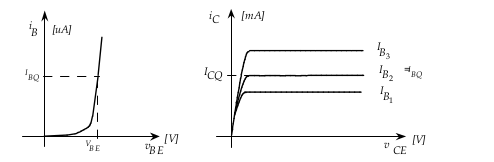
\includegraphics[scale=0.75]{TBJ.png}
						\caption{Curvas características}
					\end{center}
				\end{figure}				
			
			
			
\pagebreak
\end{document}
